\documentclass[encoding=utf8,british]{tumphthesis}
% \documentclass[pstricks,siunitx,addfonts,theorem,font=palatino,british]{tumphthesis}

% Das folgende Paket dient lediglich dazu, den Blindtext "Lorem ipsum ..."
% auszugeben und kann in einer echten Abschlussarbeit natürlich weggelassen 
% (oder auskommentiert) werden.

\usepackage{graphicx}
\usepackage[font={small}]{caption}
\usepackage[font={small}]{subcaption}
\usepackage{units}
%\usepackage{capt-of}
\usepackage{subfig}
\usepackage{csquotes}
%\usepackage{natbib}
\usepackage{physics}
\usepackage[compat=1.1.0]{tikz-feynman}
\tikzset{/tikzfeynman/warn luatex=false}

%%%%%%%%%%%%%%%%%%%%%%%%%%%%%%%%%%%%%%%%%%%%%%%%%%%%%%%%%%%%%%%%%%%%%%%%%%%%%%%%
%
% new commands
%              for units, dbd, spacings, literature,
%                  experiments and equipment, codes, and isotopes 
%
% 2013-06-29 / pg    to be used in drafts, SC or GSTR
%%%%%%%%%%%%%%%%%%%%%%%%%%%%%%%%%%%%%%%%%%%%%%%%%%%%%%%%%%%%%%%%%%%%%%%%%%%%%%%%
\usepackage{amssymb}     % packages called in main file, e.g. gstr-template.tex
\usepackage{marvosym}    % symbols for EURO
\usepackage{upgreek}     % for upright greek letters in units
% units                  %%%%%%%%%%%%%%%%%%%%%%%%%%%%%%%%%%%%%%%%%%%%%%%%%%%%%%%
%
\newcommand{\versionabb}  {version 11.0 dated 20161109}
%
\newcommand{\ctsper}      {cts/(keV$\cdot$kg$\cdot$yr)}
\newcommand{\ctsperee}    {cts/(keV$_{ee}\cdot$kg$\cdot$yr)}
\newcommand{\ctsperrec}   {cts/(keV$_{rec}\cdot$kg$\cdot$yr)}
\newcommand{\zctsper}     {{$10^{-2}$~cts/(keV$\cdot$kg$\cdot$yr)}}
\newcommand{\tctsper}     {{$10^{-2}$~cts/(keV$\cdot$kg$\cdot$yr)}}
\newcommand{\pIbi}        {{$10^{-2}$~cts/(keV$\cdot$kg$\cdot$yr)}}
\newcommand{\dctsper}     {{$10^{-3}$~cts/(keV$\cdot$kg$\cdot$yr)}}
\newcommand{\pIIbi}       {{$10^{-3}$~cts/(keV$\cdot$kg$\cdot$yr)}}
\newcommand{\biperton}    {{1~cts/(keV$\cdot$t$\cdot$yr)}}
\newcommand{\vctsper}     {{$10^{-4}$~cts/(keV$\cdot$kg$\cdot$yr)}}
\newcommand{\ctsperx}     {$\frac{10^{-3}\rm cts}{\rm keV\cdot kg \cdot yr}$}
\newcommand{\kgy}         {{kg$\cdot$yr}}
\newcommand{\kgyr}        {{kg$\cdot$yr}}
\newcommand{\kevkgyr}     {{keV$\cdot$kg$\cdot$yr}}
\newcommand{\cum}         {{m$^3$}}
\newcommand{\mubq}        {{$\upmu$Bq}}
\newcommand{\mum}         {{$\upmu$m}}
\newcommand{\mus}         {{$\upmu$s}}
%\newcommand{\mubqperkg}   {{$\frac{\upmu\mathrm{Bq}}{\mathrm{kg}}$}}
\newcommand{\mubqperkg}   {{${\upmu\mathrm{Bq}}/{\mathrm{kg}}$}}
%
\def\cpowten#1#2{{$#1\cdot10^{#2}$}}
\def\powten#1{{$10^{#1}$}}
\newcommand{\baseT}[2]{\mbox{$#1{\cdot}10^{#2}$}}
\newcommand{\baseTsolo}[1]{$10^{#1}$}
%
\newcommand{\C}           {$^\circ$C}
\newcommand{\al}          {$\alpha$}
\newcommand{\be}          {$\beta$}
\newcommand{\ga}          {$\gamma$}
\newcommand{\gam}         {$\gamma$}
\newcommand{\gammas}      {$\gamma${s}}
\newcommand{\gline}       {$\gamma$ line}
\newcommand{\glines}      {$\gamma$ lines}
\newcommand{\gray}        {$\gamma$ ray}
\newcommand{\grays}       {$\gamma$ rays}
\newcommand{\qbb}         {{$Q_{\beta\beta}$}}
\newcommand{\upqbb}       {Q$_{\upbeta\upbeta}$}
\newcommand{\Qbb}         {{$\text{Q}_{\beta\beta}$}}
\newcommand{\thalfzero}   {${T^{0\nu}_{1/2}}$}
\newcommand{\thalftwo}    {${T^{2\nu}_{1/2}}$}
\newcommand{\thalfmajo}   {{${T^{0\nu \chi }_{1/2}}$}}
\newcommand{\nmez}        {${\cal M}^{0\nu}$}
\newcommand{\nmet}        {${\cal M}^{2\nu}$}
\newcommand{\mbb}         {${\langle m_{\beta\beta}\rangle}$}
\newcommand{\nPlus}       {n$^+$ electrode}
\newcommand{\pPlus}       {p$^+$ electrode}
\newcommand{\aoe}         {$A/E$}
\newcommand{\order}[1]    {\mbox{$\mathcal{O}$(#1)}}
% dbd                     %%%%%%%%%%%%%%%%%%%%%%%%%%%%%%%%%%%%%%%%%%%%%%%%%%%%%%
\newcommand{\bbno}        {{$0\nu\beta\beta$}}
\newcommand{\onbb}        {{$0\nu\beta\beta$}}
\newcommand{\onbbchi}     {{$0\nu\beta\beta\chi$}}
\newcommand{\nnbb}        {{$2\nu\beta\beta$}}
\newcommand{\uponbb}      {{$0\upnu\upbeta\upbeta$}}
\newcommand{\upnnbb}      {{$2\upnu\upbeta\upbeta$}}
\newcommand{\twonu}       {{$2\nu\beta\beta$}}
\newcommand{\onecec}      {{$0\nu\rm{ECEC}$}}
\newcommand{\nnecec}      {{$2\nu\rm{ECEC}$}}
% other usefull           %%%%%%%%%%%%%%%%%%%%%%%%%%%%%%%%%%%%%%%%%%%%%%%%%%%%%%
\newcommand{\tlive}       {\mbox{$t_{live}$}}
\newcommand{\flive}       {\mbox{$f_{live}$}}
\newcommand{\fge}         {\mbox{$f_{Ge}$}}
\newcommand{\fgesix}      {\mbox{$f_{76}$}}
\newcommand{\fgesixi}     {\mbox{$f_{76,i}$}}
\newcommand{\actmass}     {\mbox{$M_{act}$}}
\newcommand{\ssmass}      {\mbox{$M_{76}$}}
\newcommand{\factmass}    {\mbox{$f_{av}$}}
\newcommand{\factmassi}   {\mbox{$f_{av,i}$}}
\newcommand{\factvol}     {\mbox{$f_{av}$}}
\newcommand{\factvoli}    {\mbox{$f_{av,i}$}}
\newcommand{\subssix}     {\mbox{$_{76}$}}
\newcommand{\subssixi}    {\mbox{$_{76,i}$}}
\newcommand{\subav}       {\mbox{$_{av}$}}
\newcommand{\subavi}      {\mbox{$_{av,i}$}}
%\newcommand{\ }
%% spacings for tables etc %%%%%%%%%%%%%%%%%%%%%%%%%%%%%%%%%%%%%%%%%%%%%%%%%%%%%
\newcommand{\bal}         {\rule{10mm}{0.2mm}}
\newcommand{\balf}        {\rule{10mm}{2mm}}
\newcommand{\tabta}       {\rule[-1,5mm]{0mm}{7,5mm}}
\newcommand{\tabtag}      {\rule[-3mm]{0mm}{9mm}}
\newcommand{\up}          {\rule{0mm}{5mm}}
\newcommand{\down}        {\rule[-2mm]{0mm}{3mm}}
% for literature
\newcommand{\etal}        {\textit{et al.}}
\newcommand{\bulitem}     {\item[{\large$\bullet$}]}
\newcommand{\prep}        {\textit{Preprint}}
\newcommand{\NIM}         {Nucl.~Instr.~Meth.}
\newcommand{\PRB}         {Phys.~Rev.~B}
\newcommand{\mpik}        {\mbox{MPI-K}}
\newcommand{\mpip}        {\mbox{MPI-P}}
% experiments and equipment  %%%%%%%%%%%%%%%%%%%%%%%%%%%%%%%%%%%%%%%%%%%%%%%%%%%
\newcommand{\gerda}       {\textsc{Gerda}}
\newcommand{\G}           {{\mbox{\textsc{Gerda}}}}
\newcommand{\GERDA}       {\mbox{\sc Gerda}}  
%
\newcommand{\lngs}        {{\mbox{\textsc{Lngs}}}}
\newcommand{\LNGS}        {{\mbox{\sc Lngs}}}
\newcommand{\WT}          {water tank}
%\newcommand{\ln}          {LN}            is already defined !!!!!
\newcommand{\lar}         {LAr}
\newcommand{\geni}        {{\mbox{\textsc{Genius}}}}
\newcommand{\gdl}         {\textsc{Gdl}}
\newcommand{\gerdalarge}  {\textsc{Gerda-LArGe}}
\newcommand{\bege}        {{\sc BEGe}}
\newcommand{\phaseone}    {Phase~I}
\newcommand{\phasetwo}    {Phase~II}
\newcommand{\phasetwop}   {Phase~II$^+$}
\newcommand{\PI}          {Phase\,I}
\newcommand{\PII}         {Phase\,II}

%\newcommand{\gerdanext}   {\textsc{Gerda}\,200}
\newcommand{\gerdanext}   {{\sc{Gerda-upgrade}}}


%\newcommand{\LARGE}{\mbox{{\sc LArGe}}}  don't do this, this is a LATEX command
\newcommand{\LArGe}       {\textsc{LArGe}}
\newcommand{\SUB}         {{\mbox{\text{SUB}}}}
\newcommand{\Gerdella}    {{\mbox{\textsc{Gerdella}}}}
\newcommand{\GeMPI}       {Ge\textsc{MPI}}
%\newcommand{\GEMPI}       {Ge\textsc{MPI}}
\newcommand{\GEMPI}       {Ge\textsc{mpi}}
%    other exps.          %%%%%%%%%%%%%%%%%%%%%%%%%%%%%%%%%%%%%%%%%%%%%%%%%%%%%%
\newcommand{\majorana}    {\textsc{Majorana}}
\newcommand{\Majorana}    {{\mbox{\textsc{Majorana}}}}
\newcommand{\MAJORANA}    {{\sc Majorana}}
\newcommand{\eureca}      {{\sc Eureca}}
\newcommand{\igex}        {\textsc{Igex}}
\newcommand{\IGEX}        {{\mbox{\textsc{Igex}}}}
\newcommand{\hdm}         {\textsc{HdM}}
\newcommand{\HdM}         {\mbox{\textsc{HdM}}}  
\newcommand{\HDM}         {\mbox{\textsc{HdM}}}  
\newcommand{\BX}          {\mbox{\textsc{Borexino}}}
\newcommand{\borex}       {\mbox{\textsc{Borexino}}}
\newcommand{\borexino}       {\mbox{\textsc{Borexino}}}
\newcommand{\EUROBALL}    {\textsc{Euroball}}
\newcommand{\ICARUS}      {\textsc{Icarus}}
\newcommand{\LENS}        {\textsc{Lens}}
\newcommand{\STRAW}       {\textsc{Straw}}
\newcommand{\Gallex}      {\textsc{Gallex}}
\newcommand{\LVD}         {{\mbox{\textsc{Lvd}}}}
\newcommand{\GNO}         {{\mbox{\textsc{Gno}}}}
\newcommand{\KAMLAND}     {{\mbox{\textsc{KAMland}}}}
\newcommand{\CUORI}       {{\mbox{\textsc{Cuoricino}}}}
\newcommand{\CUORE}       {{\mbox{\textsc{Cuore}}}}
\newcommand{\cuore}       {{\mbox{\textsc{Cuore}}}}
\newcommand{\AGATA}       {{\mbox{\textsc{Agata}}}}
\newcommand{\WMAP}        {{\mbox{\textsc{Wmap}}}}
\newcommand{\NEMO}        {{\mbox{\textsc{Nemo}}}}
\newcommand{\KATRIN}      {{\mbox{\textsc{Katrin}}}}
\newcommand{\MOON}        {{\mbox{\textsc{Moon}}}}
\newcommand{\EXO}         {{\mbox{\textsc{Exo}}}}
\newcommand{\GEM}         {{\mbox{\textsc{Gem}}}}
\newcommand{\CAMEO}       {{\mbox{\textsc{Cameo}}}}
\newcommand{\COBRA}       {{\mbox{\textsc{Cobra}}}}
\newcommand{\CRYOGENM}    {{\mbox{\textsc{Cryogenmash}}}}
\newcommand{\xenon}       {{\mbox{\textsc{Xenon}}}}
\newcommand{\Xenon}       {{\mbox{\textsc{Xenon}}}}
\newcommand{\taiga}       {{\mbox{\textsc{Taiga}}}}
% codes                   %%%%%%%%%%%%%%%%%%%%%%%%%%%%%%%%%%%%%%%%%%%%%%%%%%%%%%
\newcommand{\geant}       {\textsc{Geant4}}
\newcommand{\GEANT}       {\textsc{\mbox{{Geant}}}}
\newcommand{\rootv}       {\textsc{Root}}
\newcommand{\CERN}        {{\mbox{\textsc{Cern}}}}
\newcommand{\mage}        {\textsc{MaGe} }
\newcommand{\gelatio}     {\textsc{Gelatio}}
\newcommand{\mgdo}        {\mbox{MGDO}}
\newcommand{\tier}        {\textsc{Tier}}
% isotopes                %%%%%%%%%%%%%%%%%%%%%%%%%%%%%%%%%%%%%%%%%%%%%%%%%%%%%%
\newcommand{\gesix}       {{$^{76}$Ge}}
\newcommand{\geseven}     {{$^{77}$Ge}}
\newcommand{\gefour}      {{$^{74}$Ge}}
\newcommand{\gethree}     {{$^{73}$Ge}}
\newcommand{\gess}        {{$^{76}$Ge}}
\newcommand{\gesf}        {{$^{74}$Ge}}
\newcommand{\geenr}       {{$^{\rm enr}$Ge}}          %$^{\rm enr}$Ge
\newcommand{\genat}       {{$^{\rm nat}$Ge}}
\newcommand{\gedep}       {{$^{\rm dep}$Ge}}
\newcommand{\geox}        {{GeO$_2$}}
\newcommand{\enrgecoax}   {{$^{\rm enr}$Ge-coax}} 
\newcommand{\nuc}[2]      {{$^{#2}$\rm #1}}

\newcommand{\cosix}       {{$^{60}$Co}}
\newcommand{\radzzs}      {{$^{226}$Ra}}
\newcommand{\thzza}       {{$^{228}$Th}}
\newcommand{\tlzna}       {{$^{208}$Tl}}
\newcommand{\kvn}         {{$^{40}$K}}
\newcommand{\kvz}         {{$^{42}$K}}
\newcommand{\Am}          {$^{241}$Am}
\newcommand{\Rn}          {$^{222}$Rn}
\newcommand{\Ra}          {$^{226}$Ra}
\newcommand{\Po}          {$^{210}$Po}
\newcommand{\Ar}          {$^{39}$Ar}
\newcommand{\Kr}          {$^{85}$Kr}
\newcommand{\Xe}          {$^{133}$Xe}
\newcommand{\Ba}          {$^{133}$Ba}
\newcommand{\Bi}          {$^{214}$Bi}
\newcommand{\Yb}          {$^{176}$Yb}
\newcommand{\Fe}          {$^{55}$Fe}
\newcommand{\Th}          {$^{228}$Th}
\newcommand{\Tl}          {$^{208}$Tl}
\newcommand{\Ul}          {$^{235}$U}
\newcommand{\Uh}          {$^{238}$U}
\newcommand{\Be}          {$^7$Be}
\newcommand{\YO}          {Yb$_2$O$_3$}
\newcommand{\Co}          {$^{60}$Co}
%%%%%%%%%%%%%%%%%%%%%%%%%%%%%%%%%%%%%%%%%%%%%%%%%%%%%%%%%%%%%%%%%%%%%%%%%%%%%%%%
\newcommand{\exposure}    {\mbox{$\cal E$}}
\newcommand{\effqual}     {\mbox{$\varepsilon_{qcut}$}}
\newcommand{\effpsd}      {\mbox{$\varepsilon_{psd}$}}
\newcommand{\effres}      {\mbox{$\varepsilon_{res}$}}
\newcommand{\efffep}      {\mbox{$\varepsilon_{fep}$}}
\newcommand{\effquali}    {\mbox{$\varepsilon_{qcut,i}$}}
\newcommand{\effpsdi}     {\mbox{$\varepsilon_{psd,i}$}}
\newcommand{\effresi}     {\mbox{$\varepsilon_{res,i}$}}
\newcommand{\efffepi}     {\mbox{$\varepsilon_{fep,i}$}}
%
\newcommand{\effmuon}     {\mbox{$\varepsilon_\mu$}}
\newcommand{\effmurej}    {\mbox{$\varepsilon_{rej}$}}
\newcommand{\effmureji}   {\mbox{$\varepsilon_{rej,i}$}}
%%%%%%%%%%%%%%%%%%%%%%%%%%%%%%%%%%%%%%%%%%%%%%%%%%%%%%%%%%%%%%%%%%%%%%%%%%%%%%%%

%new
\newcommand{\thalfzeroLimitFreq} [3] {\thalfzero$\,>#1\cdot$\powten{#2}\,{yr} (#3\,\% C.L.)}
\newcommand{\thalfzeroSens}      [2] {\thalfzero$\,>#1\cdot$\powten{#2}\,{yr}}
\newcommand{\thalfzeroLimitPII}      {\thalfzeroLimitFreq{5.2}{25}{90}}
\newcommand{\thalfzeroSensPII}       {\thalfzeroSens{4.0}{25}}
\newcommand{\bi}                 [2] {#1$\cdot$\powten{#2}\,\ctsper}
\newcommand{\biError}            [4] {\bi{#1$^{+#2}_{-#3}$}{#4}}
\newcommand{\biPIIbege}              {\biError{0.7}{1.1}{0.5}{-3}}
\newcommand{\biPIIcoax}              {\biError{3.5}{2.1}{1.5}{-3}}


\setcounter{tocdepth}{1}
\setcounter{secnumdepth}{1}

\makeatletter
\renewcommand*{\chapterformat}{%
  \mbox{\chapapp~\thechapter\autodot:\enskip}%
}
\makeatother


%\usepackage{draftwatermark}
%\SetWatermarkScale{3}

% Die Metadaten der Abschlussarbeit werden auf dem Deckblatt gedruckt und
% in dem PDF eingetragen.
\subject{Bachelor Thesis}
%\title{Analysis of Kr85 concentration in the liquid argon of \gerda\ Phase II}
\title{Determination of the Specific \Kr\ Activity in the Liquid Argon of \gerda\ Phase II}
%\subtitle{\foreignlanguage{british}{Title in English}}
\author{Moritz Neuberger}
\date{7 ~August, 2018}

%\cooperators{Max-Planck-Institut für Physik}

% Auf der Rückseite des Deckblatts können Themensteller, Zweitgutachter 
% und Tag der mündlichen Prüfung vermerkt werden.
\lowertitleback{Erstgutachter (Themensteller): Prof.\ S.~Schönert\\
Zweitgutachter: Prof.\ H.~Kroha\\
Betreuer: C.\ Wiesinger}


%-------------------------------------------------------------------------------
%\usepackage[BCOR=10mm,DIV=12,headinclude=false,footinclude=false]{typearea}
\areaset[10mm]{160mm}{230mm}
\setlength{\voffset}{10mm}
\usepackage[pdftex,draft=false,debug=false]{hyperref}
\usepackage[utf8]{inputenc}
\usepackage[T1]{fontenc}
\usepackage[german,american]{babel}
%\usepackage[ansinew]{inputenc}
\usepackage{cite}
%\usepackage{eurosym}
\usepackage{marvosym}  %EURO symbols
\usepackage{graphicx}
\usepackage{epsfig}
\usepackage{multicol,graphics,verbatim}
\usepackage{longtable}
\usepackage{colortbl}
\usepackage{rotating}  
\usepackage{multirow}
\usepackage{booktabs}  %better hlines in tables
\usepackage{nicefrac}  % for nice 1/2 sign
\usepackage{calc}      % for parbox = including indented paragraph
\usepackage{amssymb,amsthm,amsmath}
\usepackage{units}
\usepackage{upgreek}   %  for upright greek letters in units
\usepackage{ifthen}
\usepackage{lineno}
\usepackage{lipsum}
\usepackage{amsmath}
\usepackage{capt-of}
\modulolinenumbers[5]
%%%%%%%%%%%%%%%%%%%%%%%%%%%%%%%%%%%%%%%%%   switch on/off line numbers
\linenumbers                            %   comment to switch off
%%%%%%%%%%%%%%%%%%%%%%%%%%%%%%%%%%%%%%%%%   switch off figures
\usepackage{ifthen}                     %   
\newboolean{makefigures}                %   declaration
\setboolean{makefigures}{true}          %   definition    on  == true
%\setboolean{makefigures}{false}        %   definition    off == false
%%%%%%%%%%%%%%%%%%%%%%%%%%%%%%%%%%%%%%%%%

\itemsep -4pt
\renewcommand{\floatpagefraction}{0.09}

%tables
\usepackage{array}
\newcolumntype{L}[1]{>{\raggedright\let\newline\\\arraybackslash\hspace{0pt}}m{#1}}
\newcolumntype{C}[1]{>{\centering\let\newline\\\arraybackslash\hspace{0pt}}m{#1}}
\newcolumntype{R}[1]{>{\raggedleft\let\newline\\\arraybackslash\hspace{0pt}}m{#1}}              % packages/settings
%\include{\gerda\-abbreviations} % for definitions see:  abbreviations.tex
%-------------------------------------------------------------------------------

%%%%%%%%%%%%%%%%%%%%%%%%%%%%%%%%%%%%%%%%%%%%%%%%%%%%%%%%%%%%%%%%%%%%%%%%%%%%%%%%
% -----------------------------------------------------  DEFINE YOUR REPORT  ---
%%%%%%%%%%%%%%%%%%%%%%%%%%%%%%%%%%%%%%%%%%%%%%%%%%%%%%%%%%%%%%%%%%%%%%%%%%%%%%%%
%\newcommand{\repnumber}  {GSTR-18-0xx}    % REPNUMBER (yy->year, 0xx->running number)
%\newcommand{\repdate}    {August 8, 2018} % DATE
%\newcommand{\titleheader}{Analysis of \Kr concentration in the liquid argon of \gerda\ Phase II} % TITLE
%%%%%%%%%%%%%%%%%%%%%%%%%%%%%%%%%%%%%%%%%%%%%%%%%%%%%%%%%%%%%%%%%%%%%%%%%%%%%%%%
%%%%%%%%%%%%%%%%%%%%%%%%%%%%%%%%%%%%%%%%%%%%%%%%%%%%%%%%%%%%%%%%%%%%%%%%%%%%%%%%

%\setlength\parindent{0pt}
% --------------------------------------------------------  begin document   ---
\begin{document}
\selectlanguage{british}
\frontmatter
\maketitle


% --------------------------------------------------------  begin title page  --
%\begin{titlepage}
% --------------------------------------------------------- logo /header -------
%\vspace*{20mm}
%\begin{center}
%{\Large\textbf{\titleheader}}
%\vspace*{10mm}

%%%%%%%%%%%%%%%%%%%%%%%%%%%%%%%%%%%%%%%%%%%%%%%%%%%%%%%%%%%%%%%%%%%%%%%%%%%%%%%%
% ----------------------------------------------------  DEFINE YOUR AUTHORS  ---
%%%%%%%%%%%%%%%%%%%%%%%%%%%%%%%%%%%%%%%%%%%%%%%%%%%%%%%%%%%%%%%%%%%%%%%%%%%%%%%%
%Moritz Neuberger, Christoph Wiesinger$^o$), Steffan Schönert$^o$)
%\vspace*{5mm}

% Address:  (select the appropriate ones and change letters if needed) 
%$^a$)  INFN Laboratori Nazionali del Gran Sasso  and Gran Sasso Science Institute, Assergi,  Italy\\[1mm]
%$^b$)  INFN Laboratori Nazionali del Sud, Catania, Italy\\[1mm]
%$^c$)  Institute of Physics, Jagiellonian University, Cracow, Poland\\[1mm]
%$^d$)  Institut f{\"u}r Kern- und Teilchenphysik Technische Universit{\"a}t Dresden, Dresden, Germany\\[1mm]
%$^e$)  Joint Institute for Nuclear Research, Dubna, Russia\\[1mm]
%$^f$)  European Commission, JRC-Geel, Geel, Belgium\\[1mm]
%$^g$)  Max-Planck-Institut f{\"u}r Kernphysik, Heidelberg, Germany\\[1mm]
%$^h$)  Universit{\`a} di Milano Bicocca, Milan, Italy\\[1mm]  
%$^i$)  INFN Milano Bicocca, Milan, Italy\\[1mm]                                     
%$^j$)  Universit{\`a} degli Studi di Milano e INFN Milano, Milan, Italy\\[1mm]                                 
%$^k$)  Institute for Nuclear Research of the Russian Academy of Sciences, Moscow, Russia\\[1mm]                 
%$^l$)  Institute for Theoretical and Experimental Physics, NRC ``Kurchatov Institute'', Moscow, Russia\\[1mm]                                
%$^m$)  National Research Centre ``Kurchatov Institute'', Moscow, Russia\\[1mm]                                       
%$^n$)  Max-Planck-Institut f{\"ur} Physik, Munich, Germany\\[1mm]                                          
%$^o$)  Physik Department E15 and Excellence Cluster Universe, Technische  Universit{\"a}t M{\"u}nchen, Munich, Germany\\[1mm]                           
%$^p$)  Dipartimento di Fisica e Astronomia dell{`}Universit{\`a} di Padova, Padova, Italy\\[1mm]         
%$^q$)  INFN  Padova, Padova, Italy\\[1mm]
%$^r$)  Physikalisches Institut, Eberhard Karls Universit{\"a}t T{\"u}bingen, T{\"u}bingen, Germany\\[1mm]       
%$^s$)  Physik Institut der Universit{\"a}t Z{\"u}rich, Z{\"u}rich, Switzerland\\[1mm] 
%\vspace*{20mm}
%%%%%%%%%%%%%%%%%%%%%%%%%%%%%%%%%%%%%%%%%%%%%%%%%%%%%%%%%%%%%%%%%%%%%%%%%%%%%%%%
%%%%%%%%%%%%%%%%%%%%%%%%%%%%%%%%%%%%%%%%%%%%%%%%%%%%%%%%%%%%%%%%%%%%%%%%%%%%%%%%

%%%%%%%%%%%%%%%%%%%%%%%%%%%%%%%%%%%%%%%%%%%%%%%%%%%%%%%%%%%%%%%%%%%%%%%%%%%%%%%%
% --------------------------------------------------  WRITE A SHORT ASTRACT  ---
%%%%%%%%%%%%%%%%%%%%%%%%%%%%%%%%%%%%%%%%%%%%%%%%%%%%%%%%%%%%%%%%%%%%%%%%%%%%%%%%
%\begin{abstract}
%Seite beabsichtigt leer gelassen.
%\end{abstract}
%%%%%%%%%%%%%%%%%%%%%%%%%%%%%%%%%%%%%%%%%%%%%%%%%%%%%%%%%%%%%%%%%%%%%%%%%%%%%%%%
%%%%%%%%%%%%%%%%%%%%%%%%%%%%%%%%%%%%%%%%%%%%%%%%%%%%%%%%%%%%%%%%%%%%%%%%%%%%%%%%
%\end{center}
%\vfill
%\end{titlepage}
%\vfill

% ---------------------------------------------------------------- settings  ---
%\pagenumbering{arabic}
%\setcounter{page}{1}
%\pagestyle{myheadings}
%\markboth{~-~~\repnumber\hfill\titleheader}{\titleheader\hfill\repnumber~~-~}
%\newpage
%----------------------------------------------------------------- body --------

% Ist die Arbeit auf Englisch verfasst, hier die Sprache umschalten. 
% Die Sprache muss als Klassenoption angegeben sein.

%\chapter{Titel des ersten Kapitels}
%\section{Erster Abschnitt}
%\lipsum[2-5]\cite{schwabl-qqi2002}

%Und noch etwas \emph{betontes}.

%\section{Zweiter Abschnitt}
%\lipsum[6] Test\cite{Setare:2013dra}
%\begin{figure}
%	\centering
%	
\includegraphics[width=\textwidth]{tumlogo}
%	\caption{\label{fig:test}Test}
%\end{figure}
%\subsection{Unterabschnitt}
%\lipsum[7]\cite{schwabl-qqi2002,schwabl-qffi2002}
%\subsubsection{Unterunterabschnitt}
%\paragraph{Absatz} \lipsum[8]


	%%%%%%%%%%%%%%%%%%%%%%%%%%%%%%%%%%%%%%%%%%%%%%%%%%%%%%%%%%%%%%%%%%%%%%%%%%%%%%%%
% ---------------------------------------------------  ADD HERE YOUR REPORT  ---
%%%%%%%%%%%%%%%%%%%%%%%%%%%%%%%%%%%%%%%%%%%%%%%%%%%%%%%%%%%%%%%%%%%%%%%%%%%%%%%%

%sources:
% 0: https://arxiv.org/pdf/1006.1718v2.pdf


\chapter*{Abstract}
The GERmanium Detector Array (\gerda) experiment tries to find evidence for the neutrino less double beta decay in \nuc{Ge}{76}.
Enriched high purity germanium detectors are used simultaneously as source and detector.
The liquid argon in which the detectors are located acts as coolant, passive shielding against radiation from the outside and as an active veto due to its scintillation capability.
Because of the extremely low background condition, \gerda\ explores half lives at about 10$^{26}$ yr.
A residual radioactive isotope in the liquid argon is \nuc{Kr}{85}.
It does not contribute to the background for \gerda's neutrinoless double beta decay search, but might influence analyses carried out at lower energies.
The aim of this thesis is to determine \Kr's specific activity.
In about 0.434$\%$ the \Kr\ decays are followed by the emission of a gamma with 514 keV.
Based on the line count of its peak in the energy spectrum of \gerda, the efficiency in the detectors to measure these gammas and the mean overall measurement time, the specific \Kr\ activity can be calculated.
By applying this method, a specific activity of $(0.508\pm0.086) \  \unit{mBq}/\unit{l}$ was determined.
A cross-check analysis facilitating the decay lifetime was carried out.
However, the presence of \nuc{Ar}{42} with a comparable lifetime did not allow a verification of the obtained result.


\begin{otherlanguage}{ngerman}
\chapter*{Zusammenfassung}
Das GERmanium Detector Array (\gerda) Experiment versucht, Beweise für den neutrinolosen doppelten Betazerfall in \nuc{Ge}{76} zu finden.
Angereicherte hochreine Germanium-Detektoren werden gleichzeitig als Quelle und Detektor eingesetzt.
Das flüssige Argon, in dem sich die Detektoren befinden, wirkt als Kühlmittel, als passive Abschirmung gegen Strahlung von Außen und als aktives Veto bedingt durch seine Szintillationsfähigkeit.
Aufgrund der extrem niedrigen Untergrundbedingung erforscht \gerda\ Halbwertszeiten bis etwa 10$^{26}$ yr.
Ein radioaktives Isotop im flüssigen Argon ist \nuc{Kr}{85}.
Es trägt nicht zum Untergrund für \gerdas\ die neutrinolose Doppel-Betazerfall-Suche bei, könnte aber Analysen bei niedrigeren Energien beeinflussen.
Das Ziel dieser Arbeit ist es, die spezifische Aktivität von \Kr\ zu bestimmen.
Ca. 0,434$\%$ aller \Kr-Zerfälle wird zusätzlich noch ein Gamma mit 514 keV zeitlich verzögert  emittiert.
Basierend auf der Anzahl an Counts im zugehörigen Peak im Energiespektrum von \gerda, der Effizienz der Detektoren, ein solches Gamma zu messen und auf der mittleren Gesamtmesszeit kann die spezifische \Kr-Aktivität berechnet werden.
Durch die Anwendung dieser Methode wurde eine spezifische Aktivität von $(0.508\pm0.086) \   \unit{mBq}/ \unit{l}$ bestimmt.
Es wurde ein Vergleichsanalyse mit Hilfe der exponentiellen Abnahme der Zählrate durchgeführt.
Die Anwesenheit von \nuc{Ar}{42} mit vergleichbarer Lebensdauer erlaubte jedoch keine Überprüfung des erhaltenen Ergebnisses.

\end{otherlanguage}

\tableofcontents

\mainmatter

\chapter{Introduction}
\label{sec:intro}
%paragraph about sec. neutrino phys

The double beta (\twonu) decay has been observed in several isotopes where single beta decay is forbidden.
However, the neutrinoless double beta (\onbb) decay will only occur when neutrinos are Majorana fermions.
Majorana particles have the characteristic of being particle and antiparticle at the same time, breaking the lepton number conservation. \cite{bilenky_massive_1987}
The physical background of all this is described in section \ref{sec:PhyBG}.
\\

The following section \ref{sec:gerda} will focus on the \gerda\ experiment.
The GERmanium Detector Array (\gerda) experiment tries to find evidence for the neutrino less double beta (\onbb) decay in \nuc{Ge}{76} \cite{agostini_background_2017}.
\onbb\ decay is known to have a very long half life.
It is therefore important to minimize background as good as possible. 
A passive shield around the detectors for suppression of external radiation as well as a scintillator around the detectors to actively reject radiation from the outside are therefore needed.
Liquid argon (LAr) is a fitting material for these requirements due to its low boiling point, its good shielding characteristics and its ability to scintillate. 
Commercial argon is extracted from the atmosphere by air liquefaction. 
Impurities can be removed by cryogenic distillation but traces of radioactive components can be left.
One residual radioactive isotope is \Kr\ and  will be discussed in section \ref{sec:Kry85}. 
\\

% what is the general aim of my Bachelor thesis
% general overview of how I'm going to do this
% ? what are my predictions ?
% What possible influence would the result of my work might have on the result of the \gerda\ experiment?

\section{Neutrino Physics}
\label{sec:PhyBG}

\subsection{Neutrinos and lepton number conservation}

Neutrinos are electrically neutral elementary particles.
They are leptons and, apart from gravity, they only interact with other particles via the weak force.
They occur in three different kinds of flavors: the electron neutrino $\nu_e$, the muon neutrino $\nu_{\mu}$ and the tau neutrino $\nu_{\tau}$.
According to the standard model neutrinos would be massless.
Neutrino oscillation, however, has shown that neutrinos are massive \cite{fukuda_evidence_1998}.
But the absolute values of their mass and whether they are Dirac or Marjoram particles are still unknown \cite{barabash_brief_2017}.
\\

The major difference between these two kinds of particles is that, in the case of Dirac particles, one can clearly identify particles and anti-particles while Majorana particles only have one kind.
In other words, Majorana particles are particle and anti-particle at the same time.
This would allow lepton number violation and point towards physics beyond the standard model.
Until now, only one possible transition is known that could identify neutrinos as Majorana particles.
This transition is referred to as a neutrinoless double beta (\onbb) decay \cite{schechter_neutrinoless_1982}.
 
%what are Majorana neutrinos



\subsection{\onbb\ Decay}
\label{sec:0nubetabeta}

The double beta (\twonu) decay describes the transition of two neutrons to two protons in the same nuclei.
The standard model of particle physics needs two electrons and two electron-antineutrinos in the final state of this process.
\begin{equation}
(A,Z) \rightarrow (A,Z+2) + 2e^- + 2\bar{\nu_e}
\end{equation} 
The corresponding diagram is drawn in figure \ref{fig:Feyn2nbb}.
It is only observable if a single beta decay is forbidden, while a \twonu\ decay is allowed.
In most cases, this is due to the fact that the initial state of the nuclei $(A,Z)$ is stronger bound than the transition state $(A,Z+1)$ and less strong than the final state $(A,Z+2)$ .
Their half lives are in the order of $10^{21}$ to $10^{26} \unit{yr}$ \cite{shirai_double_2018,barabash_brief_2017}.
\\

\WarningsOff
\begin{figure}[t!]
\centering
\begin{subfigure}{.475\textwidth}
\centering
\begin{tikzpicture}
\begin{feynman}
\vertex 					(b1) 	{\(u\)};
\vertex[right =5cm of b1] 	(b2) 	{\(u\)};

\vertex[below=1em of b1] 	(b3) 	{\(d\)};
\vertex[right=5cm of b3] 	(b4) 	{\(d\)};

\vertex[below=1em of b3] 	(b5) 	{\(d\)};
\vertex[right=2.5cm of b5] 	(b6);
\vertex[below=1em of b4] 	(b7) 	{\(u\)};

\vertex[below=7em of b5] 	(c1) 	{\(d\)};
\vertex[right =2.5cm of c1] (c2);
\vertex[below=7em of b7]	(c3) 	{\(u\)};

\vertex[below=1em of c1] 	(c4) 	{\(d\)};
\vertex[right=5cm of c4] 	(c5) 	{\(d\)};

\vertex[below=1em of c4] 	(c6) 	{\(u\)};
\vertex[right=5cm of c6] 	(c7) 	{\(u\)};

\vertex[below=2em of b7]	(e1)	{\(e^-\)};
\vertex[left=2cm of e1]		(e2);
\vertex[below=3em of e2]	(e3);
\vertex[below=3em of e1]	(e4)	{\(e^-\)};

\vertex[below= 1em of e1]	(n1)	{\(\bar{\nu_e}\)};
\vertex[above= 1em of e4]	(n2)	{\(\bar{\nu_e}\)};

\diagram
{
{[edges=fermion]
  (b1) -- (b2),
  (b3) -- (b4),
  (b5) -- (b6),
  (b6) -- (b7)
  (c1) -- (c2),
  (c2) -- (c3),
  (c4) -- (c5),
  (c6) -- (c7),
  (e2) -- (e1),
  (e3) -- (e4),
  (e3) -- (n2),
  (e2) -- (n1),
},
(b6) -- [boson, edge label'=\(W\)] (e2),
(c2) -- [boson, edge label=\(W\)] (e3),
};
\draw [decoration={brace}, decorate]  (b5.south west)--(b1.north west) node [pos=0.5, left] {\(n\)};
\draw [decoration={brace}, decorate]  (c6.south west)--(c1.north west) node [pos=0.5, left] {\(n\)};
\draw [decoration={brace}, decorate]  (c3.north east)--(c7.south east) node [pos=0.5, right] {\(p\)};
\draw [decoration={brace}, decorate]  (b2.north east)--(b7.south east) node [pos=0.5, right] {\(p\)};
\end{feynman}
\end{tikzpicture}
\subcaption{Feynman-Diagram for the $2\nu\beta\beta$-decay. Two neutrons transfer into two protons, two electrons and two electron anti-neutrinos. This decay has already been observed in 12 different nuclei \cite{barabash_brief_2017}.}
\label{fig:Feyn2nbb}
\end{subfigure}\hfill%
\begin{subfigure}{.475\textwidth}
	\centering
	\begin{tikzpicture}
	\begin{feynman}
	\vertex 					(b1) 	{\(u\)};
	\vertex[right =5cm of b1] 	(b2) 	{\(u\)};
	
	\vertex[below=1em of b1] 	(b3) 	{\(d\)};
	\vertex[right=5cm of b3] 	(b4) 	{\(d\)};
	
	\vertex[below=1em of b3] 	(b5) 	{\(d\)};
	\vertex[right=2.5cm of b5] 	(b6);
	\vertex[below=1em of b4] 	(b7) 	{\(u\)};
	
	\vertex[below=6em of b5] 	(c1) 	{\(d\)};
	\vertex[right =2.5cm of c1] (c2);
	\vertex[below=6em of b7]	(c3) 	{\(u\)};
	
	\vertex[below=1em of c1] 	(c4) 	{\(d\)};
	\vertex[right=5cm of c4] 	(c5) 	{\(d\)};
	
	\vertex[below=1em of c4] 	(c6) 	{\(u\)};
	\vertex[right=5cm of c6] 	(c7) 	{\(u\)};
	
	\vertex[below=2em of b7]	(e1)	{\(e^-\)};
	\vertex[left=2cm of e1]		(e2);
	\vertex[below=2em of e2]	(e3);
	\vertex[below=2em of e1]	(e4)	{\(e^-\)};
	
	\diagram
	{
		{[edges=fermion]
			(b1) -- (b2),
			(b3) -- (b4),
			(b5) -- (b6),
			(b6) -- (b7)
			(c1) -- (c2),
			(c2) -- (c3),
			(c4) -- (c5),
			(c6) -- (c7),
			(e2) -- (e1),
			(e3) -- (e4),
		},
		(b6) -- [boson, edge label'=\(W\)] (e2),
		(c2) -- [boson, edge label=\(W\)] (e3),
		(e2) -- [insertion=0.5] (e3),
	};
	\draw [decoration={brace}, decorate]  (b5.south west)--(b1.north west) node [pos=0.5, left] {\(n\)};
	\draw [decoration={brace}, decorate]  (c6.south west)--(c1.north west) node [pos=0.5, left] {\(n\)};
	\draw [decoration={brace}, decorate]  (c3.north east)--(c7.south east) node [pos=0.5, right] {\(p\)};
	\draw [decoration={brace}, decorate]  (b2.north east)--(b7.south east) node [pos=0.5, right] {\(p\)};
	\end{feynman}
	\end{tikzpicture}
	\subcaption{Feynman-Diagram of the $0\nu\beta\beta$-decay. Two neutrons transfer into two protons and two electrons. In this case the \0nbb\ decay is due to an exchange of a massive Majorana neutrino. This transition has not been detected yet.}
	\label{fig:Feyn0nbb}
\end{subfigure}
\caption{Feynman-Diagrams of the $0\nu\beta\beta$- and the $2\nu\beta\beta$-decay}
\end{figure}
\WarningsOn


In the case of a \onbb\ decay, no neutrinos are released:
\begin{equation}
(A,Z) \rightarrow (A,Z+2) + 2e^- 
\end{equation}
From here, it will be assumed that the \onbb\ decay is caused by an exchange of massive Majorana neutrinos as seen in \ref{fig:Feyn0nbb}.
A non zero effective neutrino mass $\left\langle m_{\beta\beta}\right\rangle^2$ can be determined from \onbb\ decay's half life \thalfzero\ when using their interdependence  of $1 / \thalfzero\ \propto \left\langle m_{\beta\beta}\right\rangle^2$ \cite{delloro_neutrinoless_2016}.
This effective neutrino mass is defined by 
\begin{equation}
\left\langle m_{\beta\beta}\right\rangle = \abs{\sum_i U_{ei}^2m_i }
\label{mBetaBeta}
\end{equation}
The PMNS mixing matrix elements $U_{\alpha i}$ originate from neutrino flavor mixing. 
Neutrino oscillation experiments have shown that neutrino flavor eigenstates $\nu_\alpha$ that couple to the W boson are a superposition of neutrino mass eigenstates $\nu_i$ \cite{fukuda_evidence_1998}.
\begin{equation}
\ket{\nu_\alpha} = \sum_i U^*_{\alpha i} \ket{\nu_i} 
\end{equation}
The value of each $U_{\alpha i}$ is defined by three mixing angles and three CP-violating phases.
The Dirac phase is always present, regardless whether the neutrino is a Majorana or Dirac particle.
The two Majorana phases only have a physical meaning for Majorana neutrinos.
Neutrino oscillation is only sensitive to the mass square differences $\Delta m^2_{ij} = m^2_i - m^2_j$ of the mass eigenstates and so far only an absolute value of $\Delta m^2_{32}$ could be determined.
This leaves three different possible scenarios to be considered in the \onbb\ decay \cite{bilenky_alternative_2017}:
\begin{enumerate}
    \item normal order ($m_1 < m_2 < m_3$)
    \item inverted order ($m_3 < m_1 < m_2$)
    \item quasi-degenerate order ($m_1 \approx m_2 \approx m_3$) in which the mass eigenvalues are much larger than the mass differences
\end{enumerate}
The effective neutrino mass as a function of the lightest mass of each mass ordering can be seen in figure \ref{fig:MassOrder}.
A \onbb\ decay may  provide new knowledge about the mass ordering, the mass scale as well as the Majorana phases. 
\\

Other attempts to measure the mass of the electron neutrino are measuring the end point of the beta decay \cite{otten_neutrino_2008}. 
A promising experiment right now is the KATRIN experiment.
The absolute mass these kinds of experiments can measure, is an incoherent mass sum as seen in equation \ref{massBeta}.
\begin{equation}
\left\langle m_{\beta}\right\rangle = \sqrt{\sum_i \abs{U_{ei}}^2m^2_i}
\label{massBeta}
\end{equation}
A third method involves cosmological observation in which the sum of the neutrino masses $\Sigma$ can be measured \cite{abazajian_cosmological_2011}:
\begin{equation}
\Sigma = \sum_i m_i
\end{equation}
From comparing these three masses it is possible to determine the Majorana phases, the individual masses of the mass eigentstates and therefore also the mass order of the neutrinos.
\\

\begin{figure}[t!]
	\centering
	\begin{minipage}[t]{.475\textwidth}
		\centering
		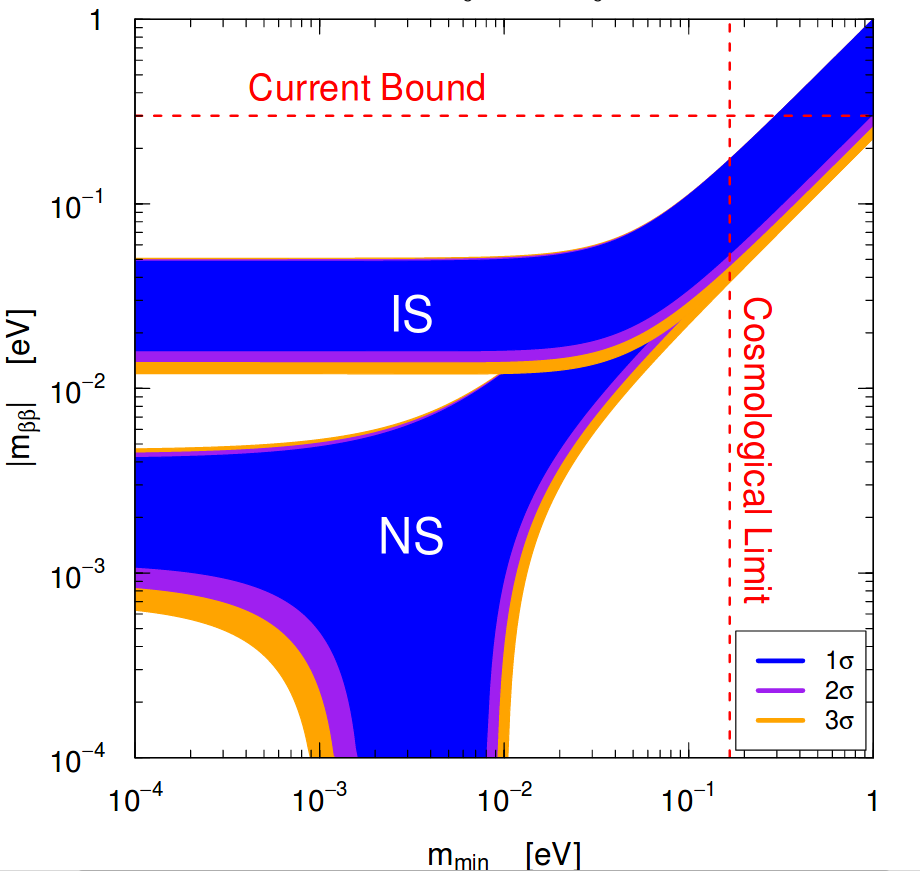
\includegraphics[width=.825\textwidth]{./Bilder/NeutrinoMassOrdering.png}
		\caption{Effective neutrino mass $\left\langle m_{\beta\beta}\right\rangle$ as a function of the smallest mass of the respective mass hierarchy. NS stands for the normal order and IS for the inverted order. Taken from \cite{bilenky_neutrinoless_2012}.}
		\label{fig:MassOrder}
	\end{minipage}\hfill%
	\begin{minipage}[t]{.475\textwidth}
		\centering
		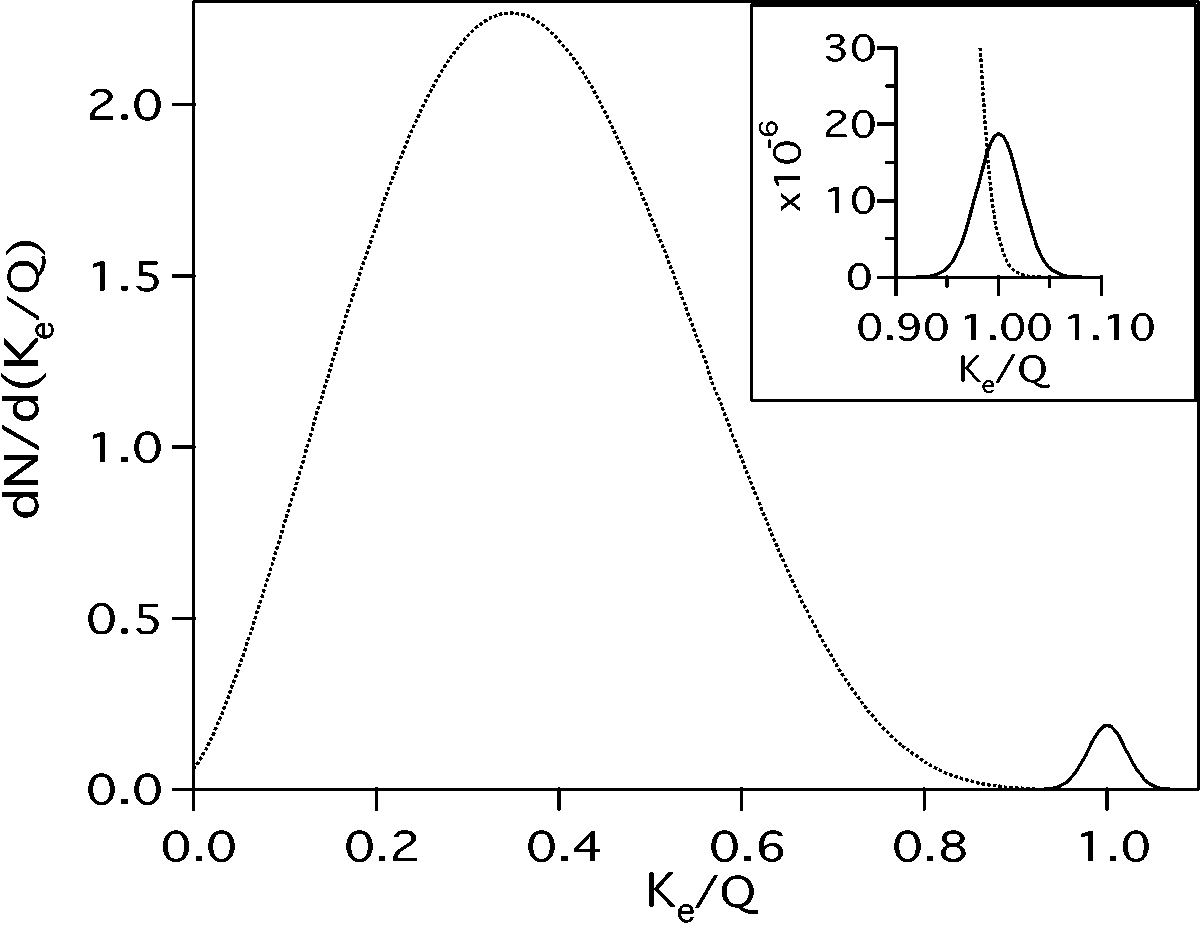
\includegraphics[width=\textwidth]{./Bilder/TheoretischesSpektrmdes0nubbDecay.png}
		\caption{Effective spectrum of a \twonu\ decay when adding the energies of the two escaping electrons.  Taken from \cite{elliott_double_2002}.}
		\label{fig:TheoSpektrum}
	\end{minipage}
\end{figure}

\subsection{Experimental methods to detect a \onbb\ decay}

The experimental signature of the \onbb\ decay is a sharp peak at the $Q_{\beta\beta}$ value of the \twonu\ decay in the effective spectrum of the two electrons (see figure \ref{fig:TheoSpektrum}).
One experimental approach consist in using a detector made of material enriched in a \onbb\ decaying isotope.
This has the advantage that the detection efficiency is maximized.
\\

Since \onbb\ decay should have a very long half-life, any background has to be minimized just to measure the resulting influence.
There are three kind of background sources which have to be considered.
\begin{enumerate}
    \item Cosmic background.
Muons and other particles shower down to the earth from the atmosphere and create background in the detectors.
Most of their influence can be suppressed by placing the experiment deep underground.
By also applying a muon veto system the most of the residual muon flux can be suppressed.
\item Natural radioactivity.
This is typically the dominant background source originating from radioactive isotopes which are naturally present in all materials.
Its influence can be suppressed by passively shielding the detectors and by the selecting of low radioactive components in the setup. 
\item The \twonu\ decay material itself.
Its impact on the background cannot be reduced by external measures or shielding.
However, by using a detector with high energy resolution or a decay material of high Q-value, its influence can be suppressed.
\end{enumerate}
\nuc{Ge}{76} has often been used in \onbb\ decay search experiment. 
As it is a semiconductor, it can be used as detector material itself.
A disadvantage of \nuc{Ge}{76} is its low Q-value of $Q_{\beta\beta} = 2039\unit{keV}$, which is lower than \nuc {Tl}{208}'s and \nuc{Bi}{214}'s end point energy\cite{barabash_brief_2017}.
It is also hard to increase the target volume compared to e.g. \nuc{Xe}{136} \cite{barabash_brief_2017}.
Its advantages, however, are its ability to be made with great intrinsic radio-purity, its high energy resolution and its high detection efficiency.
These facts outweigh the disadvantages which is the reason why it already has a long history for being used as decay material and why it was chosen for the \gerda\ experiment.
\\

%\nuc{Ge}{76} has a long history of use as decay material in \onbb\ experiments, most notably in the Heidelberg-Moscow(HdM) and the IGEX experiments.
%Both of these experiments are the predecessor experiments of \gerda\.
%With detectors made of enriched germanium plus the background reducing precautions and active vetos described above they were able to set a similar limit of the half life of the \onbb\ to $\thalfzero(\nuc{Ge}{76}) > 1.9\times10^{25}\unit{yr}$ \cite{noauthor_phys._nodate}. 
%HdM experiment actually claimed to have measured the half life of about $\thalfzero(\nuc{Ge}{76}) = 1.19\times10^{25}\unit{yr}$ , but its legitimacy has been questioned by a part of the scientific community \cite{klapdor-kleingrothaus_search_2004}.
%\\

%This is where the  \gerda\ experiment comes in.
%Its first measuring phase (\PI) was planned to verify or falsify the results of the HdM experiment using the detectors used in the HdM and the IGEX experiment.
%\PI started in November 2011 and May 2013 with a total exposure  of  $21.6 \frac{\unit{kg}}{\unit{yr}}$ and no signal of a \onbb\ observed \cite{agostini_results_2013}.
%With its results and the results from HdM and IGEX a new lower limit for the half life was able to be set at $\thalfzero(\nuc{Ge}{76})>3.0\times10^{25}$  yr  (90$\%$ C.L.)
%The second phase (\PII) with 30 new custom-made enriched detectors together with the old detectors has started measuring in late 2015 and had its latest data published !!!! hier noch ob ich das NATURE paper quoten soll!!!!!.
%A more detailed description of the construction and functionality of the \gerda\  \PII~ is the topic of the next section.

% also a bit about standard double beta decay
% differences between the standard and neutrinoless beta decay
 


\section{\gerda\ \PII}
\label{sec:gerda}

% general Information, e.g. 
% sizes 
% Gran Sasso, 
% what other  neutrino less beta decay experiments are there,

\subsection{Experimental Setup}
\label{sec:ExSetup}
The \gerda\ experiment is located in the underground Laboratori Nazionali del Gran Sasso (LNGS) of INFN, Italy.
The laboratories are located approximately 1.4 km below ground, which corresponds to a water equivalent of 3.5 km.
\gerda\ uses \nuc{Ge}{76} as \onbb\ source as well as the detector material \cite{agostini_background_2017}.
\\

The detectors are operated bare in a liquid argon (LAr) tank of 64m$^3$ volume at an working temperature of about 90K.
Its main purpose is to cool the germanium detectors down to their working temperatures and to passively shield them against external radiation originating from the outside.
LAr can also scintillate.
This is why in \PII, extra instrumentation was positioned inside the LAr tank in order to measure any light signal around the detectors.
As any \nuc{Ge}{76} decays are unlikely to create scintillation light, their signal can be used as a veto - the so-called LAr veto.
Situated around the LAr cryostat is a 590m$^3$ water tank.
Its main purpose is to shield the setup from outside radiation not only passively by absorption but also actively as a muon veto.
Situated in the water tank are 66 photomultipliers.
They detect Cherenkov light created by Muons.
Above the water tank, a clean room is installed in which the detector strings are assembled  \cite{agostini_background_2017}.  
The general setup can be seen in figure \ref{fig:gerdaSetupPII}.
\\

\begin{figure}[t!]
	\centering
	\begin{minipage}[t!]{.45\textwidth}
		\centering
		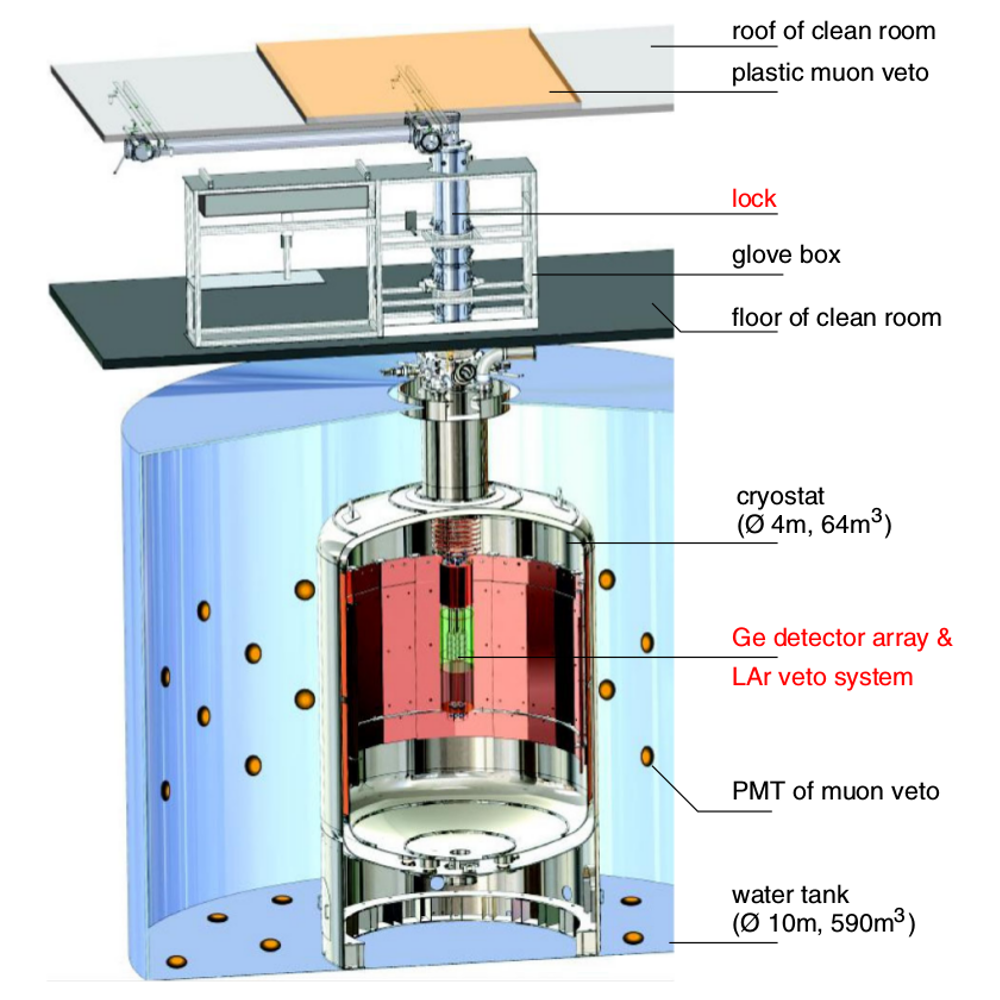
\includegraphics[height=60mm]{./Bilder/GERDAsetupPhaseII.png}
		\caption{Sketch of the \gerda\ \PII's experimental setup. The germanium detector array is placed inside a liquid argon (LAr) cryostat which itself is surrounded by a water tank. Taken from \cite{collaboration_upgrade_2018}.}
		\label{fig:gerdaSetupPII}
	\end{minipage}\hfill%
	\begin{minipage}[t!]{.45\textwidth}
		\centering
		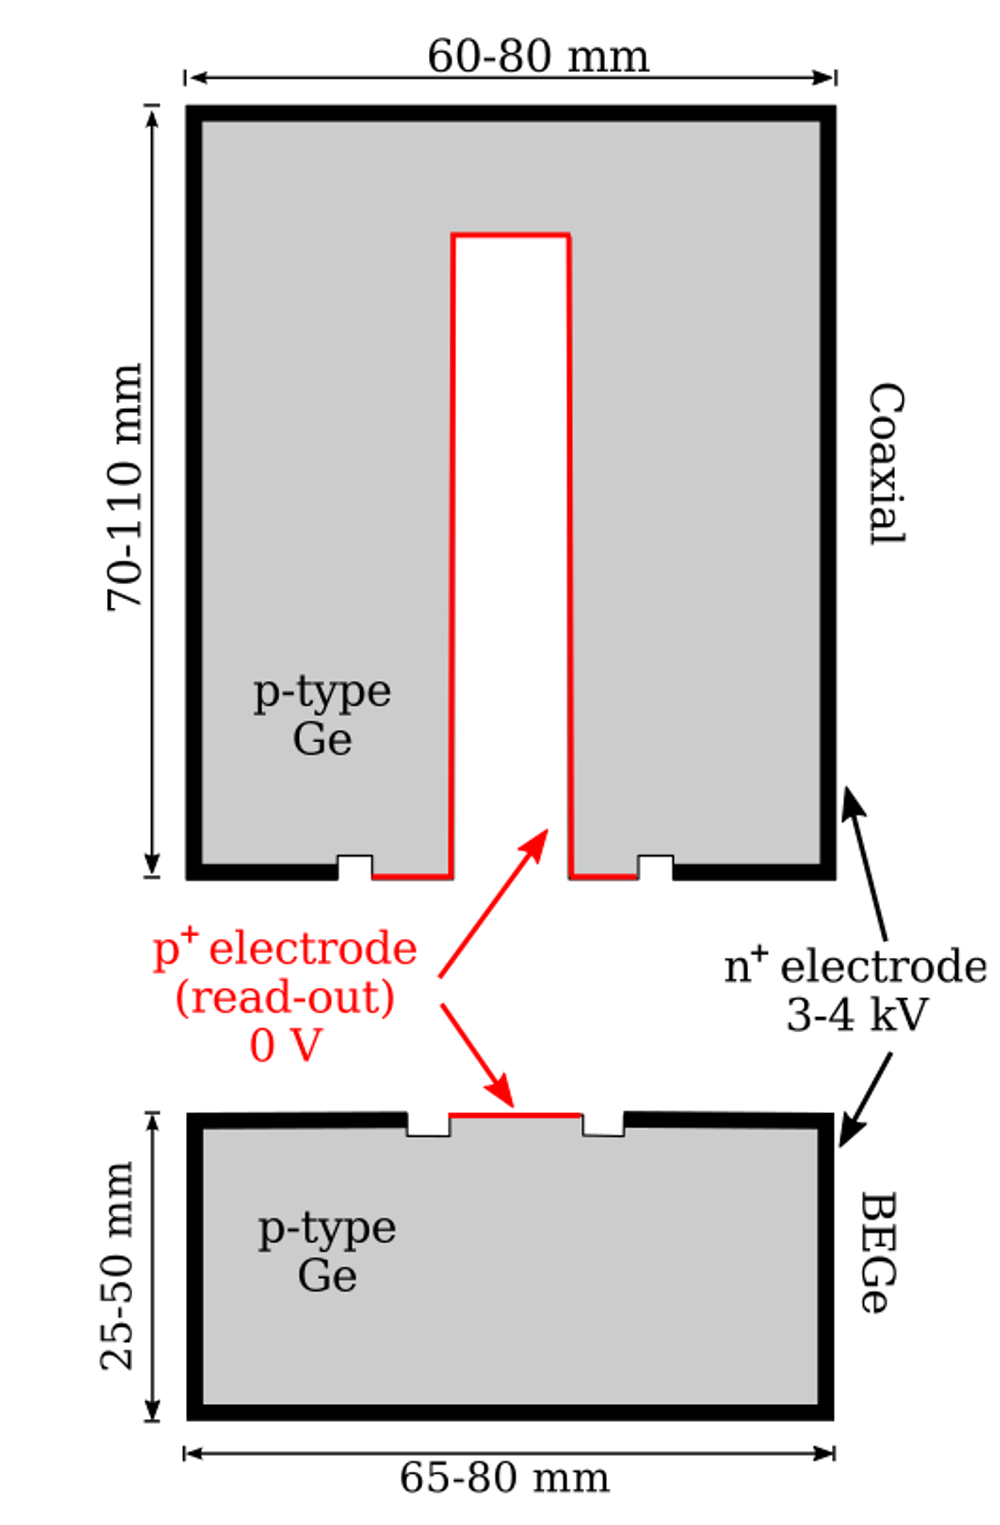
\includegraphics[height=60mm]{./Bilder/DetectorDesign.png}
		\caption{Sketch of the Semi-Coaxial (COAX) and Broad Energy Germanium (BEGe) detector designs. Taken from \cite{agostini_background_2014}.}
		\label{fig:DetcDes}
	\end{minipage}
\end{figure}

Regarding the detectors themselves, \gerda\ \PII\ uses seven semi-coaxial detectors (COAX) which have already been used in the predecessor experiments (Heidelberg-Moscow and IGEX) as well as 30 new Broad Energy Germanium detectors (BEGe).
Both detector types are made of germanium that has been enriched from 7.8$\%$ of \nuc{Ge}{76} to about 87$\%$ \cite{agostini_background_2017}.
They also share the same basic functionality.
They are made from p-type germanium material.
Both detectors have doped most of their surface 1-2mm thick n$^+$ and only a small part p$^+$ with both layers to be used as electrodes.
If an electron hole pair is created in the p doped area, the charged carriers are separated and guided to the n$^+$ or the p$^+$ layer respectively by a strong electrostatic field (3 to 4 kV) between the electrodes \cite{spieler_semiconductor_2005}.
If the pair is created in the n$^+$ layer, the hole is most likely to recombine in the $n^+$ layer due to its low mobility and, thus, creates no measurable signal.
The n$^+$ layer is therefore not active and called a dead layer.
\\

The two detectors, however, differ in their design as seen in figure \ref{fig:DetcDes}.
Moreover the detector types also differ in their mass and energy resolution.
But their design also results in a worse energy resolution due to their higher capacity compared to the BEGes \cite{agostini_production_2015}.
BEGes also allow for better pulse shape discrimination (PSD) compared to the COAX detectors.
PSD can make a statement about the creation process of the electron hole pair by looking at the shape of the signal.
It can therefore discriminate between different event topologies and acts as a veto \cite{agostini_pulse_2013}.
\\

The enriched detectors are assembled into 6 strings forming a hexagonal array together with a seventh string.
This seventh string consists of three extra coaxial detectors made of natural isotopic germanium.
However, they are not used in \gerda's main analysis.
Custom-made amplifiers also located in the liquid argon above the detectors, the analog signals of the detectors are digitized at a sampling rate of 100MHz if a triggering signal was found \cite{riboldi_cryogenic_2015}.
Every 20 seconds a charge pulse, called the test pulse, is injected into the the front-end electronics.
Its purpose is to monitor the gain stability.
The analysis of the signals is performed off-line.
Surrounding the detectors so-called nylon mini shrouds (NMS) are attached to limit the amount of LAr volume around the detectors.
These NMS are placed there to passively suppress the background created from \nuc{K}{42}\cite{agostini_background_2014}.


\iffalse
\begin{figure}[t!]
	\centering
	\begin{subfigure}{.66\textwidth}
		\centering
		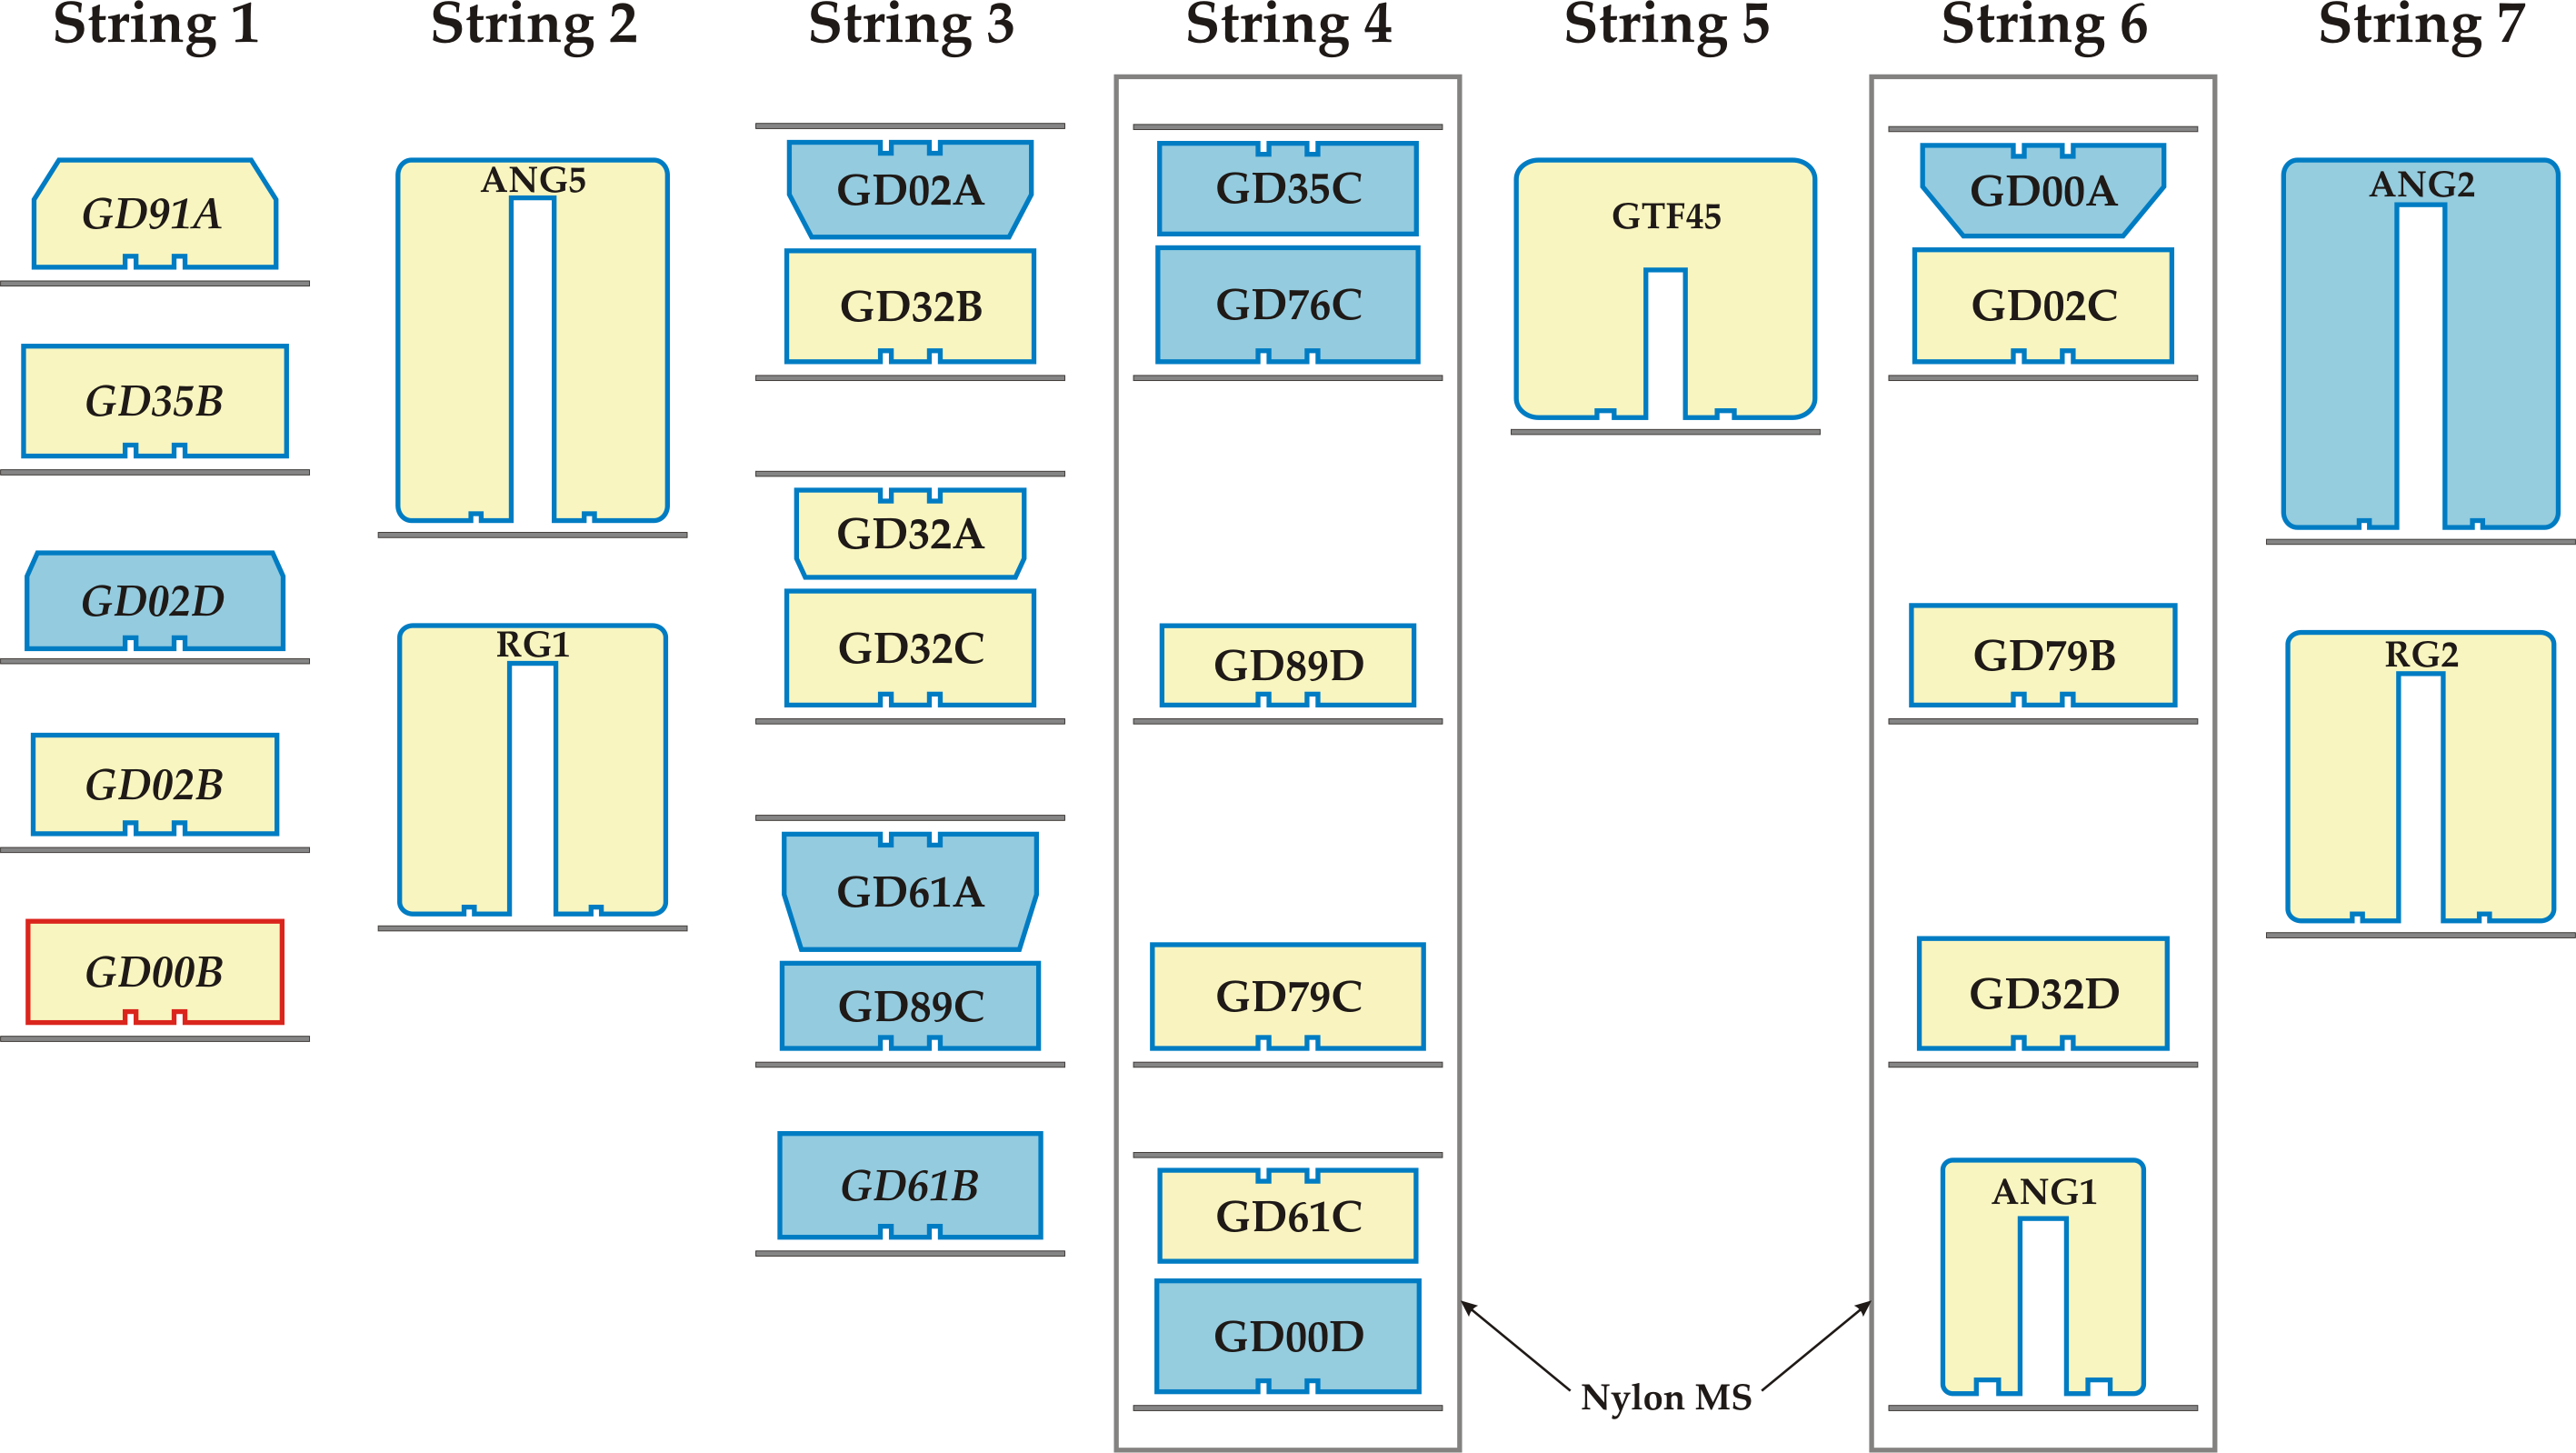
\includegraphics[width=.9\textwidth]{./Bilder/strings.png}
		\caption{}
		\label{fig:strings}
	\end{subfigure}\hfill%
	\begin{subfigure}{.30\textwidth}
		\centering
		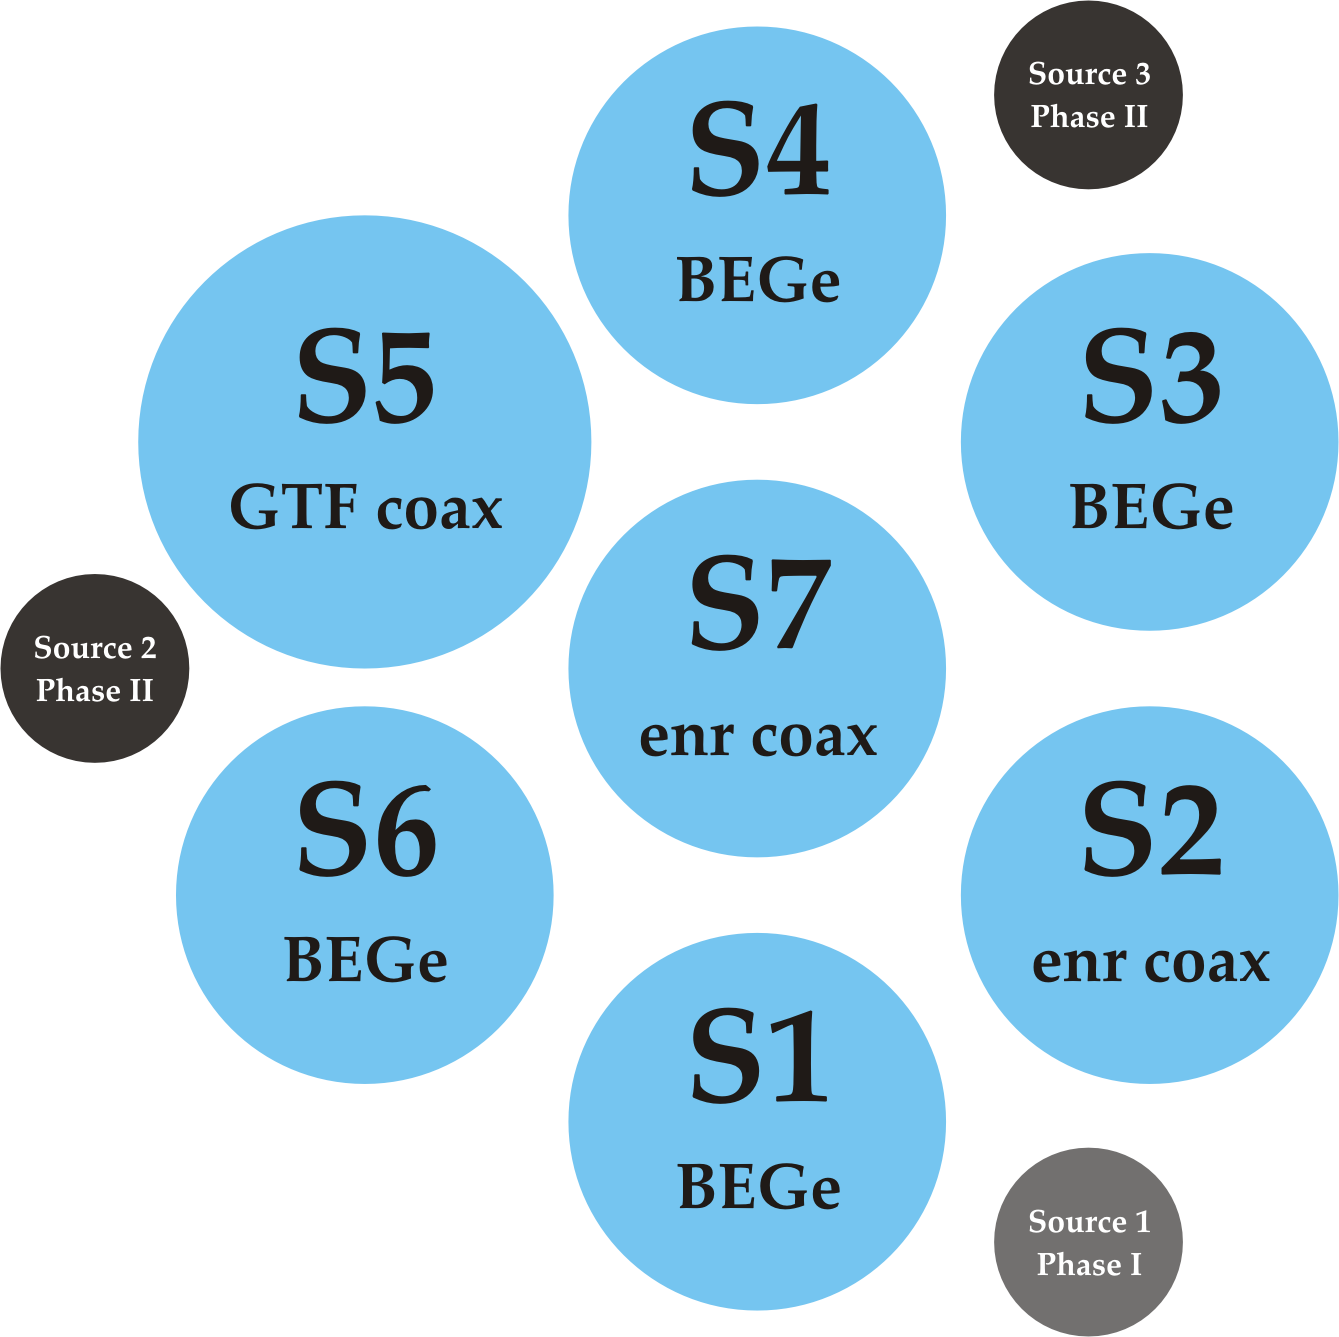
\includegraphics[width=.9\textwidth]{./Bilder/strings-top.png}
		\caption{}
		\label{fig:stringsabove}
	\end{subfigure}
\end{figure}
\fi
% well, just dump everything here
% also a bit about Tier1-4 storage of data 

\subsection{Liquid Argon as Coolant, Shielding and Scintillator} 
\label{sec:LArcoolant}


\begin{figure}[t!]
	\centering
	\begin{minipage}{.475\textwidth}
		\centering
		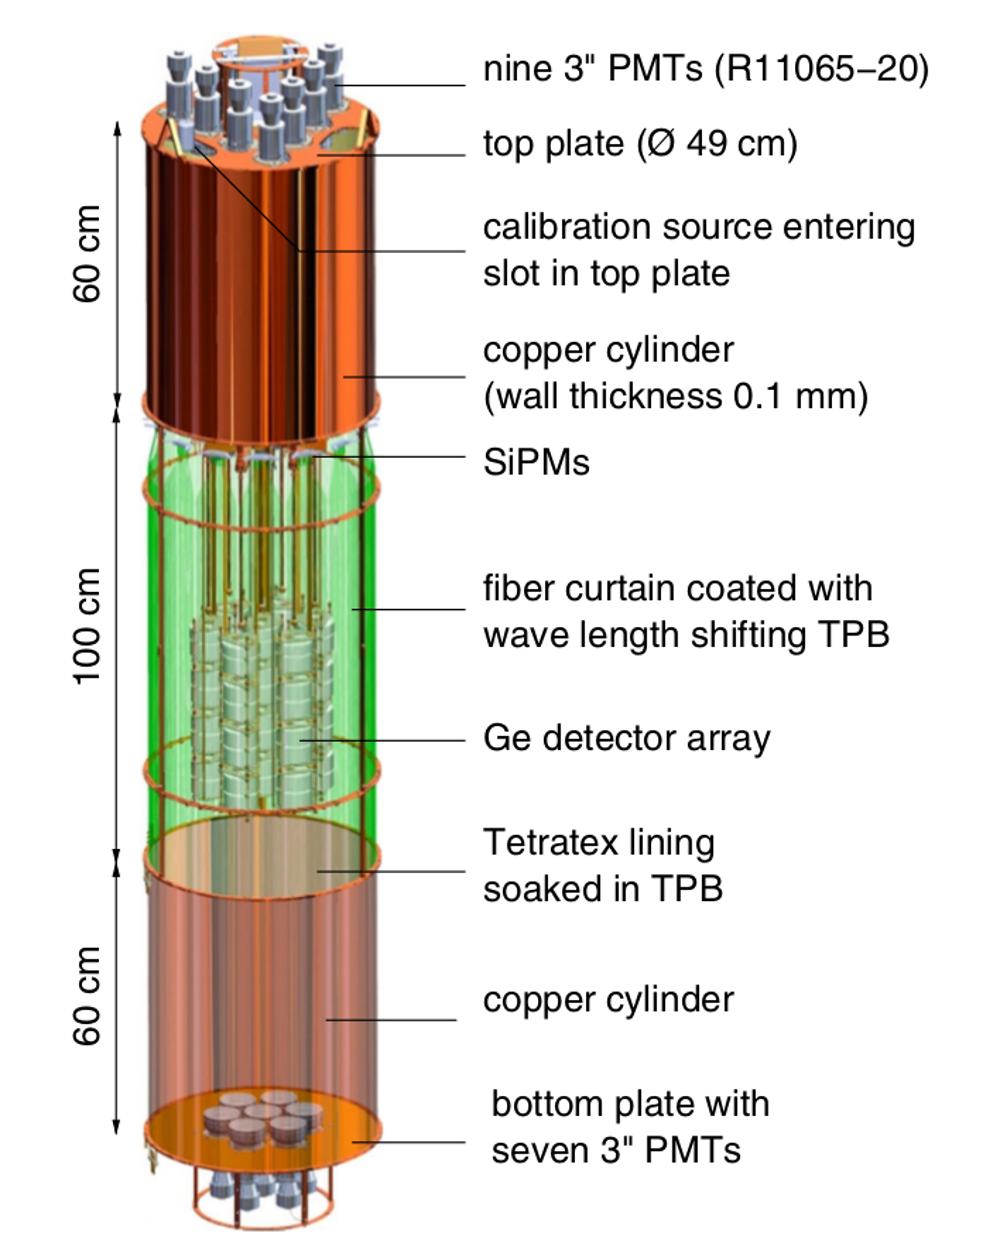
\includegraphics[width=0.6\textwidth]{./Bilder/LArVetoSetup.png}
		\caption{Sketch of the liquid agron (LAr) veto setup. 
        In the setup 16 photomultiplier tudes (PMT) and 90 silicon photomultiplers (SiPM) are installed. 
        \iffalse
        16 photomultiplier tubes (PMT) are mounted in a cylindrical copper surface at the top and bottom. 
        At the level of the detectors, the cylinder consists of fibers instead of copper. 
        They are read out at their ends by silicon photomultipliers (SiPM). 
        \fi
        Taken from \cite{collaboration_upgrade_2018}.}
		\label{fig:LArVetoSetup}
	\end{minipage}\hfill%
	\begin{minipage}{.475\textwidth}
		\centering
		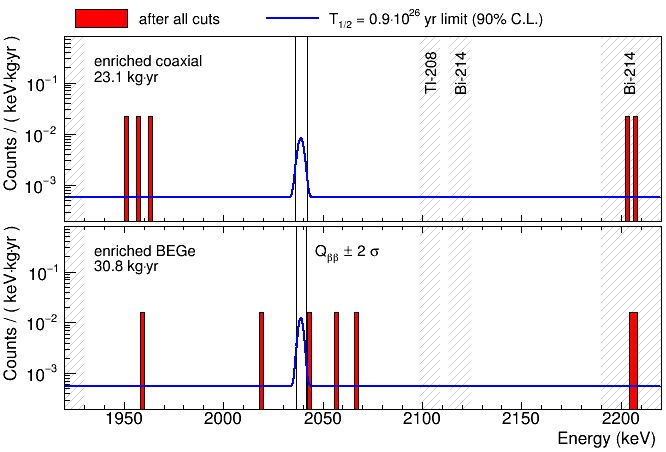
\includegraphics[width=\textwidth]{./Bilder/GerdaErgebnisse.png}
		\caption{
        Recent results from \gerda\ \PII. 
        The measured spectra in the range around \nuc{Ge}{76}'s $Q_{\beta\beta}$ value are displayed separately for the detector type in which the event was measured.  
        \iffalse
        Only one decay 2 sigma from the \onbb\ decay was found. 
        This leads to the conclusion that no \onbb\ decay was measured and a new lower limit of \thalfzero\ = $0.8\times10^{26} \unit{yr}$ (90$\%$ CL) was determined. 
        \fi
        Taken from \cite{zsigmond_new_2018}}.
		\label{fig:gerdaErgebnisse}
	\end{minipage}
\end{figure}


LAr is a good coolant due to its low boiling point.
In \gerda, it is cooled down to the working temperature of the germanium detectors at about 90 K.
LAr can also be produces with a very high purity by air separation and further distillation.
It also has good shielding capabilities of radioactive background.
It is therefore a fitting to be used in \gerda\ as coolant and ultra pure shielding material \cite{agostini_background_2017}.
Compared to other noble gases, argon also has the advantage of a very low price being easily obtained by liquefaction of air from the atmosphere \cite{olsen_improvements_nodate}.
\\

LAr has the property that scintillation light is produced when radiation excites or ionizes atoms in the material.
The excited atoms in noble liquids form dimer pairs (Ar$^*_2$).
These dimer pairs are metastable and relax with the release of a vacuum ultraviolet photon (VUV)  which have a wavelength of 128 nm \cite{olsen_improvements_nodate}.
\\

Background events often deposit energy in the argon while passing through it.
Their scintillation light around the detectors can therefore be used as a veto to reject those events.
The LAr veto system consists of a cylindrical copper shell around the germanium detectors and is equipped with 16 photomultiplier tubes (PMT), situated at the bottom and at the top of this volume.
Also, at the level of the detectors the shell is not made of copper but of wavelength shifting fibers.
These are read out by 90 silicon photomultipliers (SiPM) (see figure \ref{fig:LArVetoSetup}).
VUV has a wavelength which is so small most material absorbs it in ionization.
This is why wavelength shifting material covers the surface of the LAr veto shifting from 128nm to 400nm \cite{csathy_optical_2016}.
\\

\begin{figure}[t!]
	\centering
		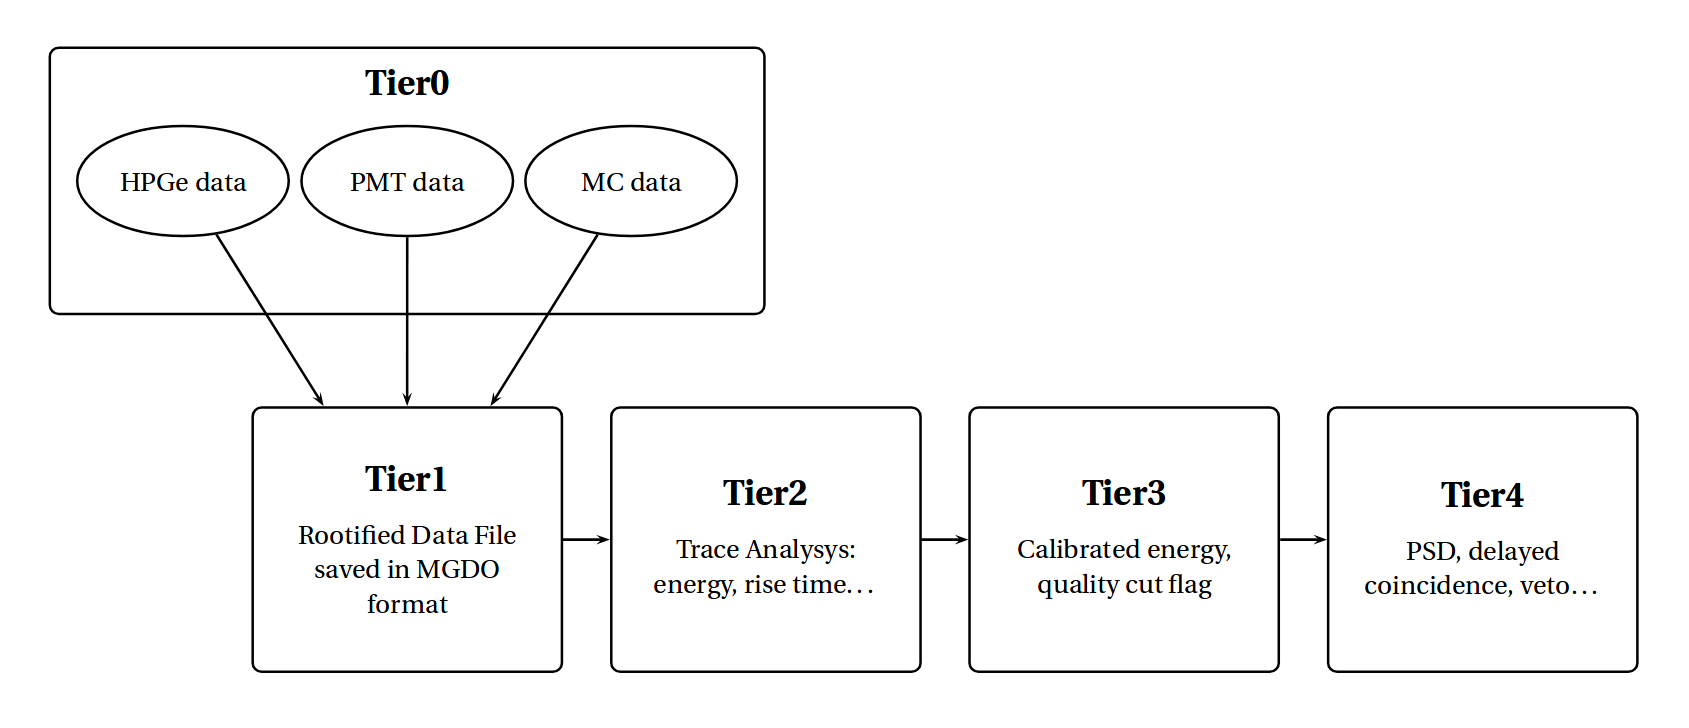
\includegraphics[width=100mm]{./Bilder/TierStructure.png}
		\caption{
		The multi-tier structure used by GELATIO. 
		Tier0 and Tier1 contain the entire raw data with the difference that Tier1 already stores the data in a TTree root structure.
		Tier2, Tier3 and Tier4 contain the resulting data of the successive analysis steps.
		Taken from \cite{agostini_gelatio:_2011}.
		}
		\label{fig:TierStructure}
\end{figure}

\subsection{Data processing and analysis}
\label{sec:DataProc}



As already mentioned, in the case of an event the digitized signals of the germanium detectors and the LAr channels are stored for further off-line analysis.
The software used for the analysis is Gerda LAyouT for Input/Output (GELATIO) being an analysis framework specialized for this task.
An advantage of it lise in its multiple level data organization as seen in figure \ref{fig:TierStructure}.
Tier0 and Tier1 store the raw data measured by the detectors, while all higher tiers contain the resulting data of the successive analysis steps.
Additional information about the analysis process can be found in \cite{agostini_gelatio:_2011} and \cite{agostini_off-line_2011}.
In this thesis only data from Tier3 and Tier4 are used.
\\

To ensure an unbiased approach to the analyzing process, all events measured in a  50 keV interval around $Q_{\beta\beta}$ were only stored without any analysis applied on them and are unable to be accessed.
Only after all parameters in the rejection process were finally defined all events of this interval will be analyzed.
Such a procedure is called a blinding process and the revealing of the blinded events an unblinding.
\\

% Mui, Mountain, Pulse shape disc.
% especially LAr-Veto 

\subsection{Recent Results}

\begin{figure}	
		\centering
	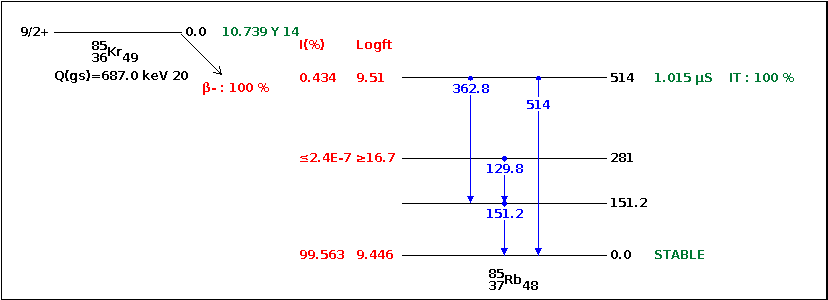
\includegraphics[width=\textwidth]{./Bilder/Kr85Decay.png}
	
	\caption{
	The decay scheme of \Kr. 
    \iffalse
    It decays via two different channels. 
    The majority of transitions end in the ground state of \nuc{Rb}{85} while 0.434$\%$ of the time \Kr\ decays into an excited state being 514 keV over the ground state. 
    The excited state has a half life of 1.015$\mu$s. It
    then relaxes directly into the ground state. 
    \fi
    Created using the decay scheme tool provided by www.nndc.bnl.gov.
	}
	\label{fig:Decay}
\end{figure}
Only recently, new data was published by \gerda\ in such an unblinding event.
In it, only one event in the proximity of the Q-value was found as shown in figure \ref{fig:gerdaErgebnisse}, however, it is more than 2 sigma from the expected peak position.
The conclusion was therefore that no evidence for a \onbb\ decay has been seen.
A new lower limit for \nuc{Ge}{76} was determined to be $\thalfzero\ > 0.9\times10^{26} \unit{yr}$ (90$\%$ CL) \cite{zsigmond_new_2018}.
Currently \gerda\ receives an upgrade and is planned to measure until 2020.
After that, the successor experiment LEGEND is planned to further investigate the \onbb\ decay in\nuc{Ge}{76}.

% what has happened so far

% short outline of approaches


\section{\Kr\ Isotope in the Atmosphere}
\label{sec:Kry85}

\Kr\ has a mass number of A = 85 and an atomic number of Z = 36.
This isotope is not stable and decays via a $\beta^-$-decay into \nuc{Rb}{85}.
The half life of this decay is 10.756 yr and has a Q-value of $Q_\beta = 687 \unit{keV}$.
\Kr's $\beta$-decay has two different probable transitions (see figure \ref{fig:Decay}).
With overwhelming 99.563$\%$, the \Kr\ decay directly populates the ground state of \nuc{Rb}{85}.
In 0.434$\%$, however, it decays via an excited state of \nuc{Rb}{85} 514 keV above the ground state.
This excited state has a half life of 1.015 $\unit{\mu s}$ and relaxes immediately into the ground state while emitting  a photon carrying the energy difference \cite{singh_nuclear_2014}.
\\

\begin{figure}[t!]
	\centering
	\ifmakefigures%
	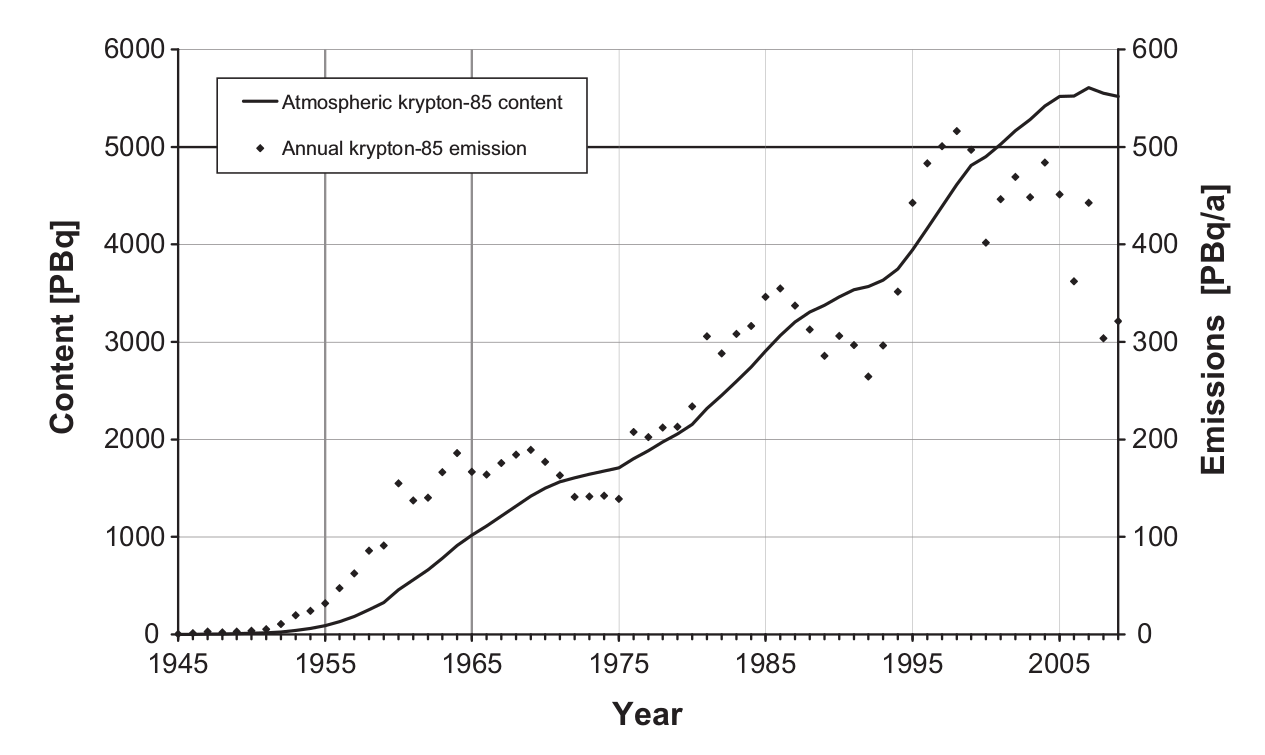
\includegraphics[width=80mm]{./Bilder/Kr85Aenderung.png}
	\fi%
	\caption{
	    \Kr's specific activity in the atmosphere between 1945 to 2009. 
	    Over this period the average specific activity in the atmosphere has increased due to man-made nuclear fission in reactors. 
		Taken from \cite{ahlswede_update_2013}.
	}
    \label{fig:Kr85Aenderung}
    
\end{figure}

The argon used in \gerda\ \PII\ was extracted from the atmosphere.
By separating argon from the other components of the air, it can easily be made very radioactively pure.
Nevertheless, a very small portion of alien elements like krypton can still be present in the extracted argon and therefore also \Kr.
\\

When investigating on how  \Kr\ got into the atmosphere, two different sources on earth can be identified.
On the one hand side, it can be created naturally in the atmosphere by an interaction of \nuc{Kr}{84} with cosmic rays.
On the other hand, the production of man-made \Kr\ from nuclear fission of \nuc{U}{235} and \nuc{Pu}{239} generates an atmospheric inventory which is about four orders of magnitude higher.
Natural production in the earth's crust is only marginal \cite{winger_new_2005}.
Krypton is a noble gas and therefore easily diffuses through everything in its way.
It rises until it reaches the atmosphere where a \Kr\ reserve is built over time.  
Due to the higher amount of nuclear power plants built in the last half century, the\Kr\ activity in the atmosphere has risen from about 1961 PBq in 1973 \cite{telegadas_atmospheric_1975} to about 5500 PBq in 2009 \cite{ahlswede_update_2013} (see figure \ref{fig:Kr85Aenderung}) .
\\

Two other experiments also using LAr are the WARP and the Darkside experiment.
In both experiments the specific activity of residual \Kr\ in the LAr was determined.
The Darkside experiment, using underground argon (UAr), has measured a specific activity of \((2.86\pm0.18) \ \unit{mBq}/\unit{l}\)  \cite{agnes_results_2016}.
This UAr has been extracted from underground reservoirs and should only have come into contact with \Kr\ from natural processes.
In the LAr of the WARP experiment, a specific \Kr\ activity of   \((160\pm130) \ \unit{mBq}/\unit{l}\) was measured \cite{benetti_measurement_2006}.
Th WARP experiment uses atmospheric argon which could be the reason why it has a higher specific activity compared to Darkside.
The aim of this thesis is to determine the specific \Kr\ activity in the LAr of \gerda\ \PII.


% where does it come from?
% what properties does it have?
% why is it important to calculate its influence on \gerda\

 
 
 
 
 
 
 
 
 
 
 
 
 
 
 
 
 
 
 
 
 
 
 
 
 
 
 
 
 
 
 
 
 
 
 
 
 
 
 
 
 
 
 
\chapter{Line Count Rate Analysis}
\label{sec:SAfrom514}

The first and more precise method to determine the specific \Kr\ activity in \gerda\ \PII\ uses the 514 keV line count rate of the \Kr\ decay.
As discussed in section \ref{sec:Kry85}, \Kr\ has a small probability of $p=0.434\%$ to decay into an excited state of \nuc{Rb}{85m}. 
When \nuc{Rb}{85m} relaxes into its ground state, it emits a photon of 514 keV energy.
The counts $N_{\mathrm{peak}}$ in the 514 keV line in the \gerda\ spectra would therefore allow to draw a conclusion concerning the amount of \Kr, as will be discussed in sections \ref{sec:prep} to \ref{sec:Fitting}. 
\\

A factor necessary for the calculation is the efficiency of the germanium detector used to detect these 514 keV gamma.
For this, a Monte Carlo simulation is needed in which $N_{\mathrm{sim}}$ gammas with an energy of 514 keV  in a  volume $V_{\mathrm{sim}}$ are simulated.
The detector efficiency for 514 keV gammas can then be calculated from dividing the simulated line count at 514 keV by the total number of  decays ($\epsilon = \Delta N/N_{\mathrm{sim}}$).
The value $1/p \epsilon V_{\mathrm{sim}}$, using the detector efficiency, the simulated volume and the probability $p$ is a conversion factor from a measured line count to the density of decays necessary to create this signal and will be calculated in section \ref{sec:MonteCarlo514}.
\\

The final value needed is the mean measuring time $\bar{t}$.
Not every detector was operational over the course of Phase II.
This is why an average measuring time for all detectors will be calculated in section \ref{sec:CalcActiv}.
With these three values, a mean specific activity $\bar{a}$ as will be shown in section \ref{sec:res}.

\begin{equation}
    \bar{a} = N_{\mathrm{peak}} \times \frac{1}{p \epsilon V_{\mathrm{sim}}} \times \frac{1}{\bar{t}}
    \label{equ:activityDieErste}
\end{equation}
The line count rate analysis is expected to generate a relatively precise estimation of the specific activity.
This is due to the 514 keV line being a clear feature which can only be traced back to \Kr.
\\


\iffalse
However, a problem of this method lies with the proximity of the \Kr\ to the 511keV peak of the positron electron annihilation. 
Its peak in the energy spectrum is expected to partially dominate over \Kr\ and does not allow for a direct measurement of the 514keV peak. 
This is not necessarily a great setback because one can just adapt the fit function to a double Gaussian peak function.
It is of interest, however, whether it is possible to completely suppers the annihilation peak without changing the 514keV photon line count.
For this one could consider using the LAr veto.
Due to the low mean energy of the escaping electron (47.65keV) of this decay, it is very unlikely that it creates any scintillating light. 
On the other hand one can expect the light of the positron electron annihilation to create a great signal in the photomultipliers.
Therefore it should be possible with the LAr veto to single out the 514keV photon events from the annihilation events.
If possible its value can be used as a cross-check for the value determined from the not filtered spectrum.

The rest of the chapter will cover the concrete implementation of the individual steps in their own sections.
\\
\fi
\section{Preparing the Spectra}
\label{sec:prep}

To determine the amount of events caused by 514 keV gammas, a fit has to be applied onto the corresponding peak in the energy spectrum.
The data used in this analysis is the fully available \gerda\ \PII\ data (run 53 to 92).
The standard \gerda\ analysis cuts where applied.
This includes data quality cuts, the Muon veto cut and the anti-coincidence cut between germanium detectors.
\\

The data was also split for the two detector types in \gerda.
This is necessary due to the differences in detector efficiency and resolution already mentioned in section \ref{sec:ExSetup}.
BEGes have a lower efficiency to detect full 514 keV gammas but show a higher energy resolution ($\Delta E_{\mathrm{BEGe}} = 2.267\unit{keV}  @ 514 \unit{keV}$) and vice versa for the COAX detectors ($\Delta E_{\mathrm{COAX}} = 2.720\unit{keV} @ 514 \unit{keV}$).
The resolutions of the two detector types were determined using the calibration spectrum as seen in appendix chapter \ref{sec:ResDetermination}.
The exposure of all BEGe detectors over the entire period of \PII\ is 30.8 kg$\cdot$yr and 28.1 kg$\cdot$yr for the COAX detectors, calculated in section \ref{sec:CalcActiv}.
\\

\begin{figure}[t!]
\centering
\begin{subfigure}{.475\textwidth}
  \centering
	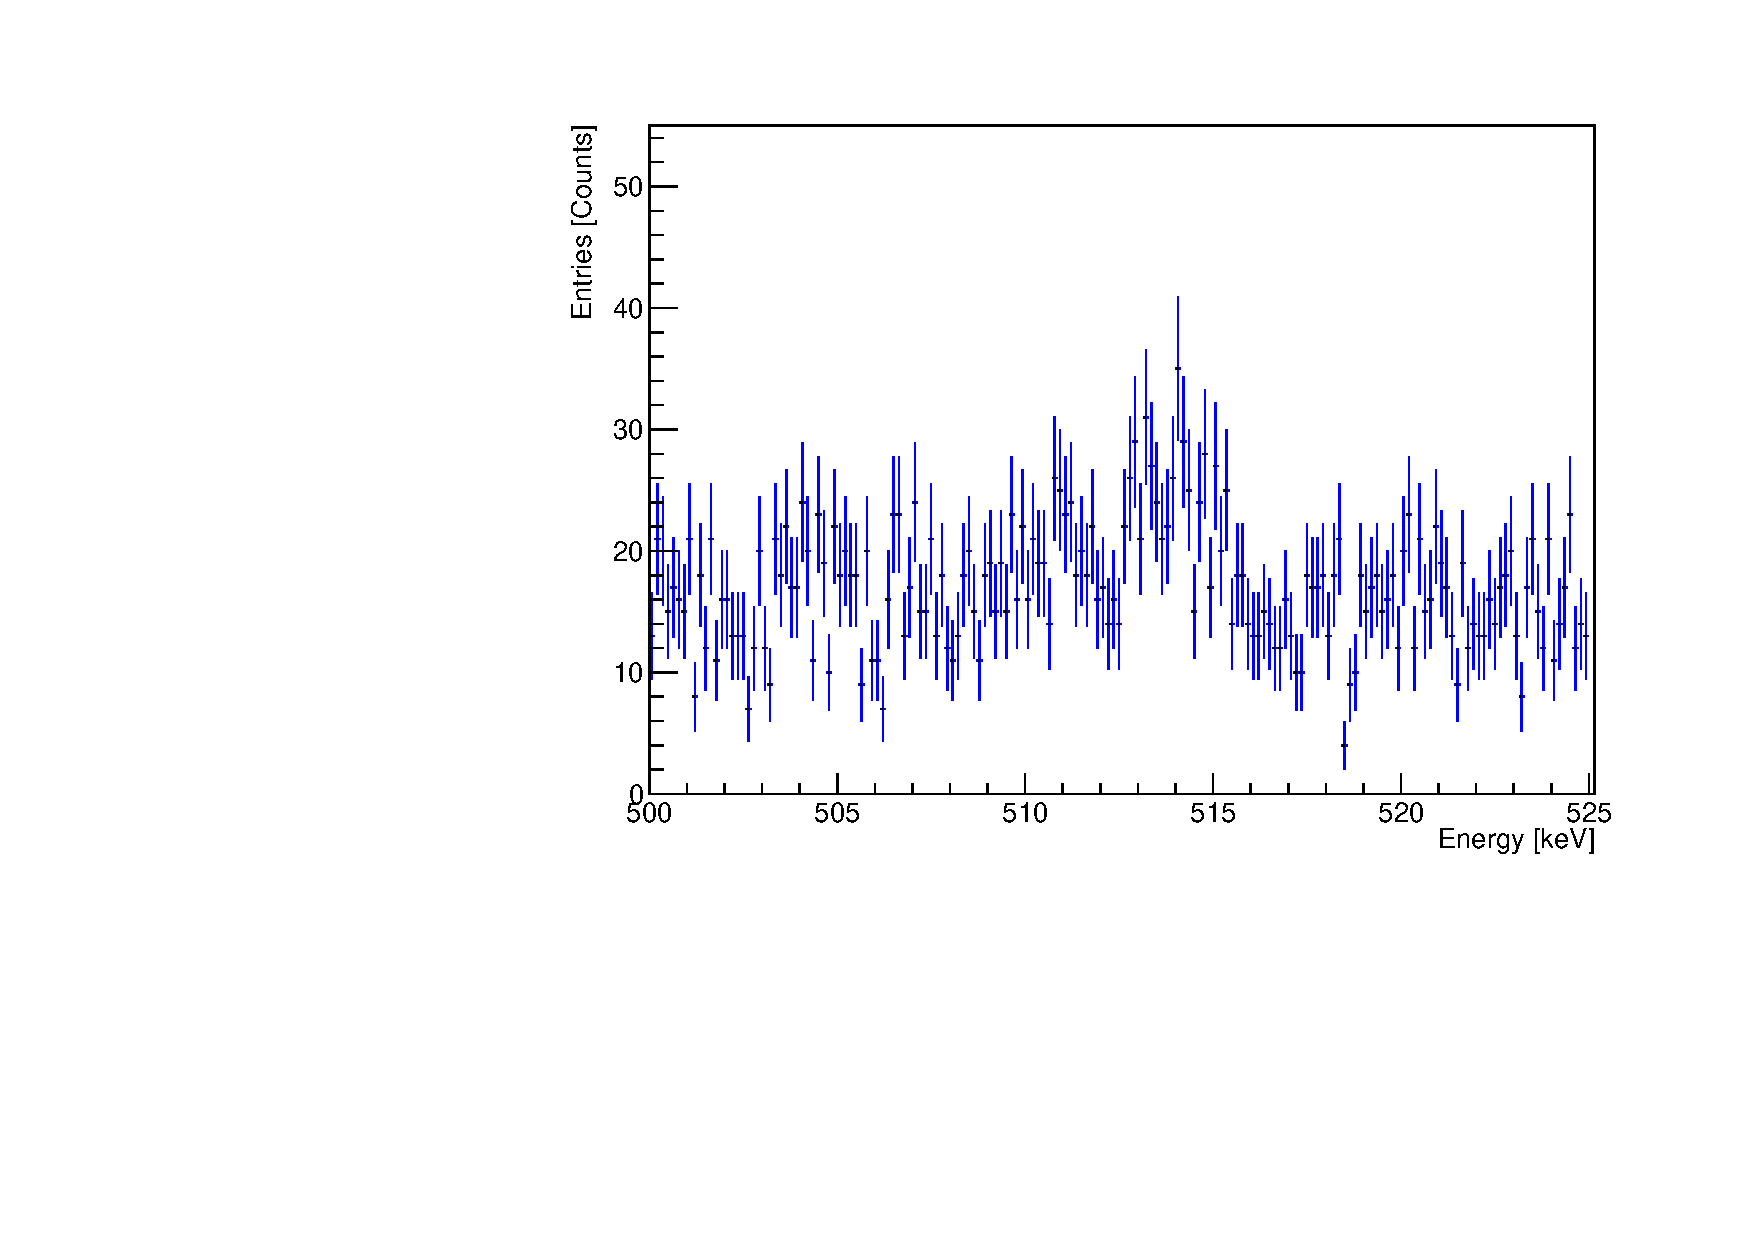
\includegraphics[width=75mm]{./Bilder/500525NoFilterBEGes.pdf}

  \caption{BEGe}
    \label{fig:NoFilterBEGes}
\end{subfigure}\hfill%
\begin{subfigure}{.475\textwidth}
  \centering
	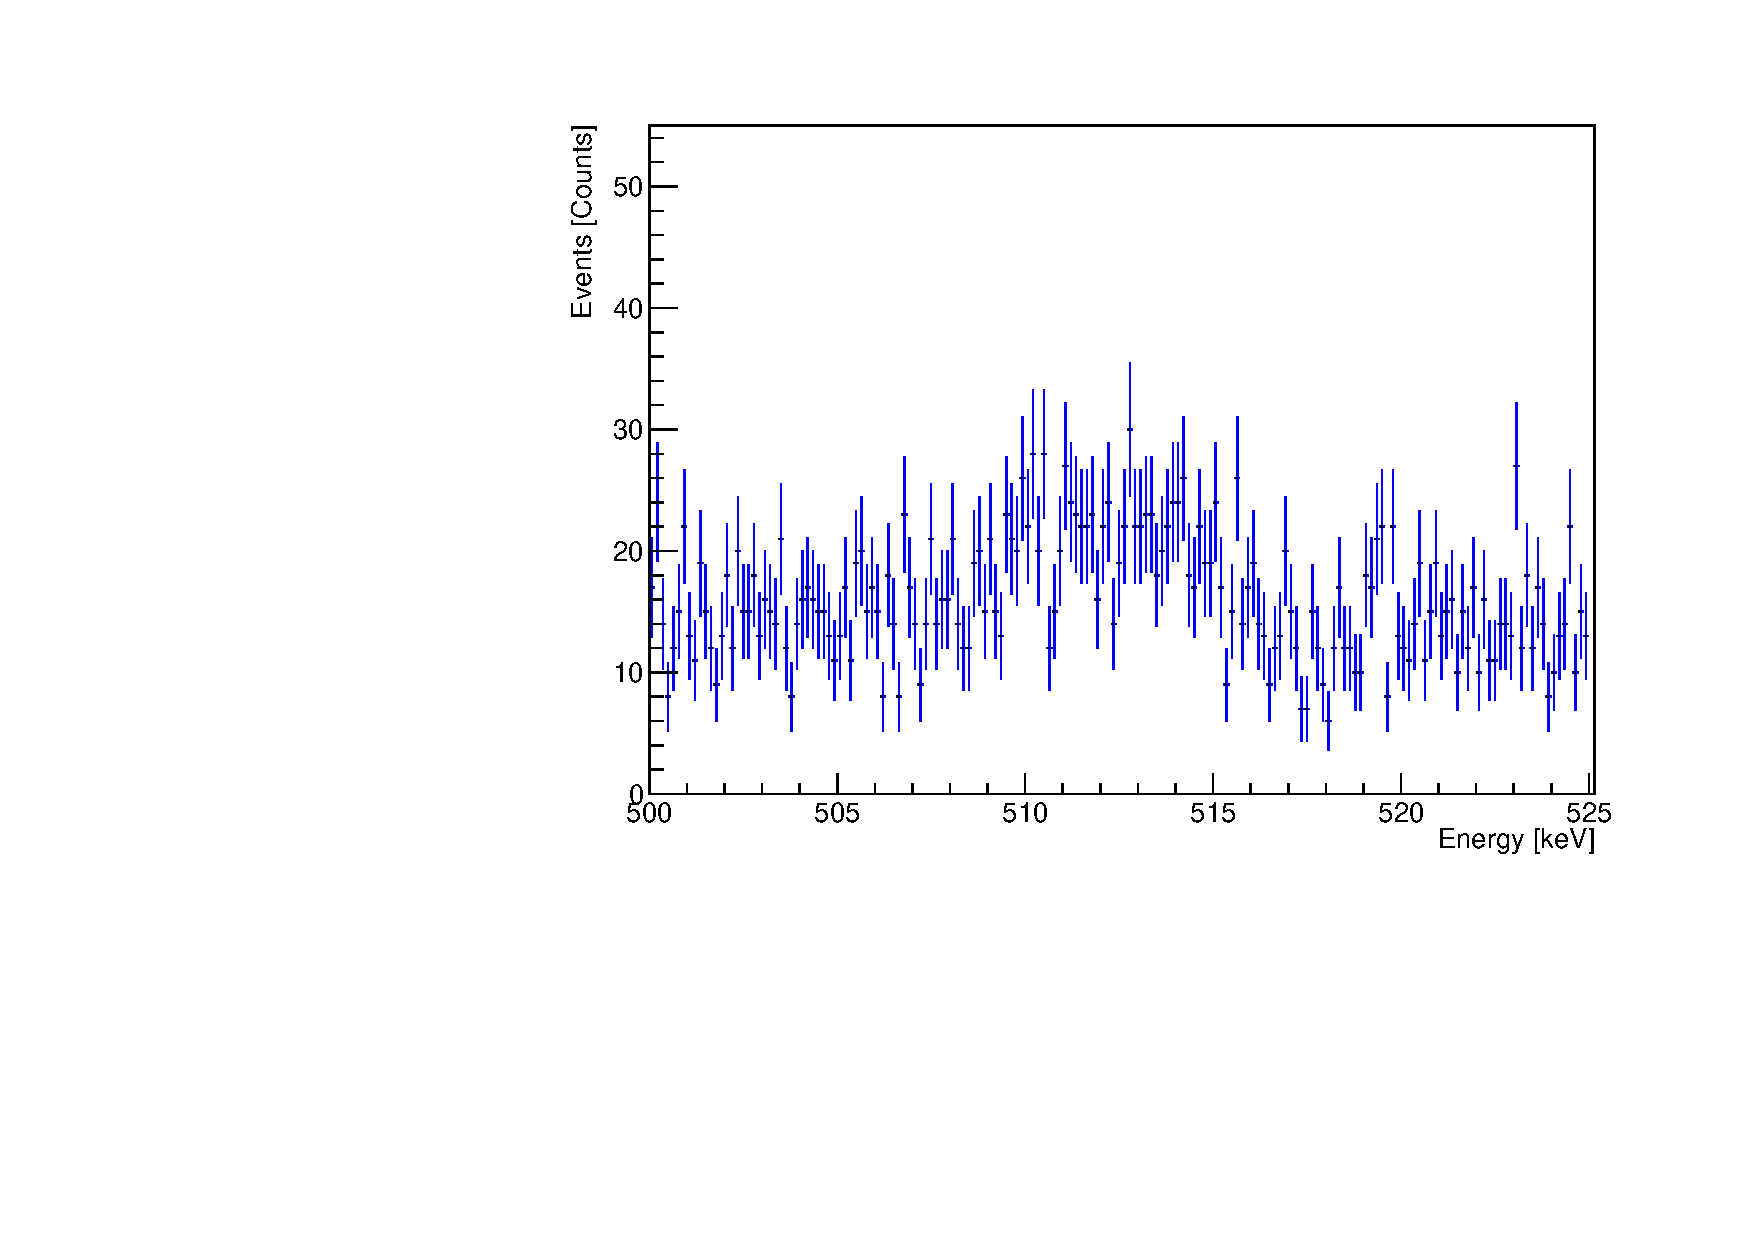
\includegraphics[width=75mm]{./Bilder/500525NoFilterCOAX.pdf}
  \caption{COAX}
  \label{fig:NoFilterCOAX}
\end{subfigure}
	\caption{
	Energy spectra after to standard \gerda\ analysis cuts between 500 and 525 keV, split by the respective detectors in which the signal was measured.
	Two deviations from the background level can be seen in both figure at 511 keV and 514 keV.
	}
			\vspace{5mm}
\end{figure}

Figures \ref{fig:NoFilterBEGes} and \ref{fig:NoFilterCOAX} show the two resulting spectra for each detector between 500 and 525 keV.
Structures deviating from the background level can be identified  at 511 keV and 514 keV.
The 511 keV deviation originates from gammas generated in positron electron annihilation events, while the 514 keV line was most likely caused by gammas created in the relaxation of \nuc{Rb}{85m} in the \Kr\ decay via this excited state.
If you examine these figures, you can already make the statement that there must be a not insignificant amount of \Kr\ in the LAr as otherwise no deviation should be visible.
\\

\iffalse
After the adjusting the spectra to a lower background level, one can now determine more precisely the number of measured events in the 514keV peaks of the corresponding detectors (see figure \ref{fig:NoFilterBEGes} for the BEGe and \ref{fig:NoFilterCOAX} for the spectra of the COAX detectors). 
In these two spectra one can see two peaks - one at 511keV that corresponds to the positron electron annihilation events and one at 514keV that corresponds to the photons from the relaxation of \nuc{Rb}{85m}.
From this we can already claim that there must be a non negligible amount of \Kr\ in the liquid argon.
Otherwise no peak should have been able to be measured. 
The difference in resolution as discussed above can be seen in the fact that in the BEGe diagram the two peaks have a smaller full width at half maximum (FWHM).
Compared to the COAX detectors their peaks can easily be distinguished.  
\fi




\iffalse
Another possible approach suppress the annihilation peak using an almost ideal filter and fit the resulting one peak spectrum with the original fit function.
As mentioned above the LAr Veto should be a good candidate for such a filter.

In this thesis both approaches will be applied separately and later their results compared.
Hopefully both will end up delivering the same result as no \Kr\ caused event should make a notable light signal.
But this probability is not zero which is why some events of the 514keV peak might also trigger the veto.
This would result in a smaller peak amplitude and with it a lower specific activity than the actual value. 
Whether or not a rejection process using the LAr veto would be useful in this analysis or not is the topic of the following section.
\\
\fi

\section{Annihilation Peak Suppression}
\label{sec:APS}


\begin{figure}[t!]
\centering
\begin{subfigure}{0.475\textwidth}
	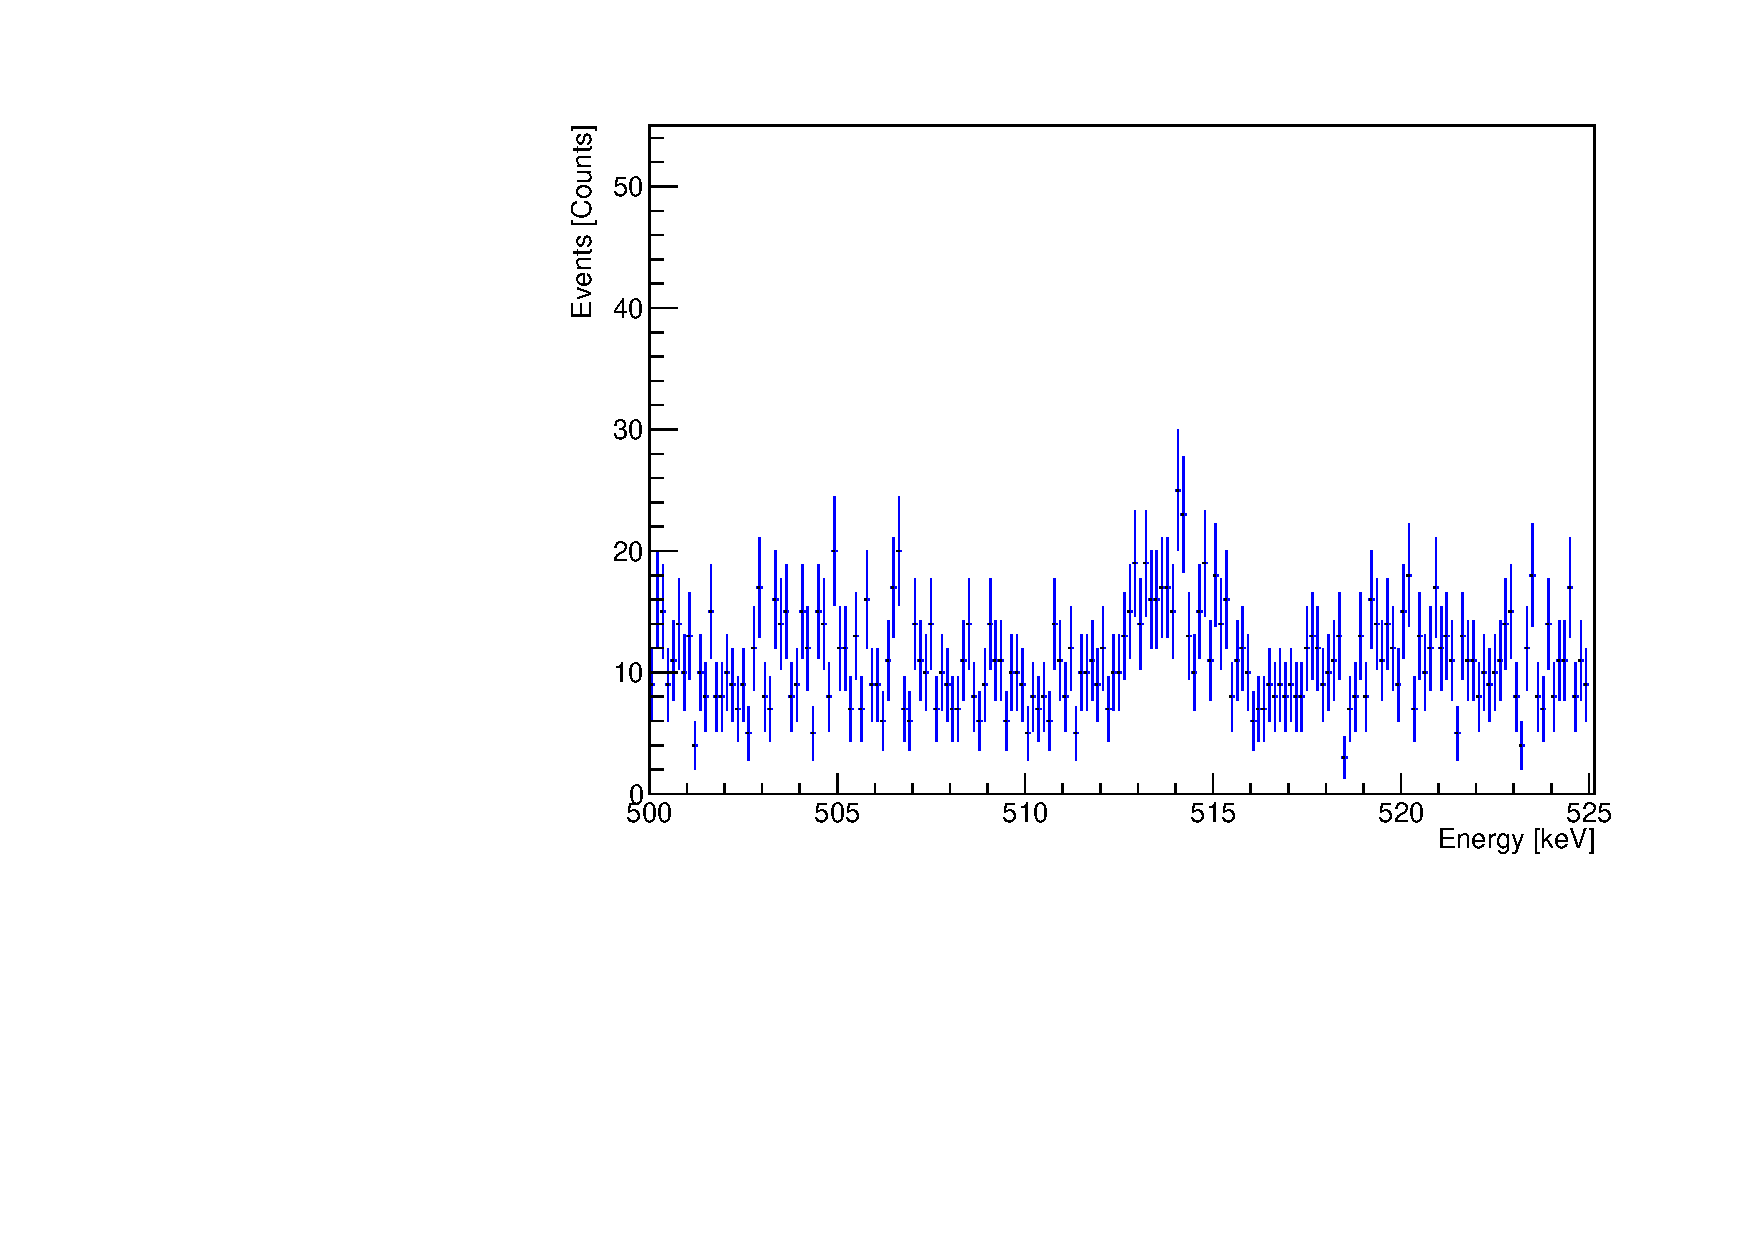
\includegraphics[width=75mm]{./Bilder/500525LArVetoBEGes.pdf}
    \caption{BEGes}
  \label{fig:LArBEGes}
\end{subfigure}\hfill%
\begin{subfigure}{0.475\textwidth}
	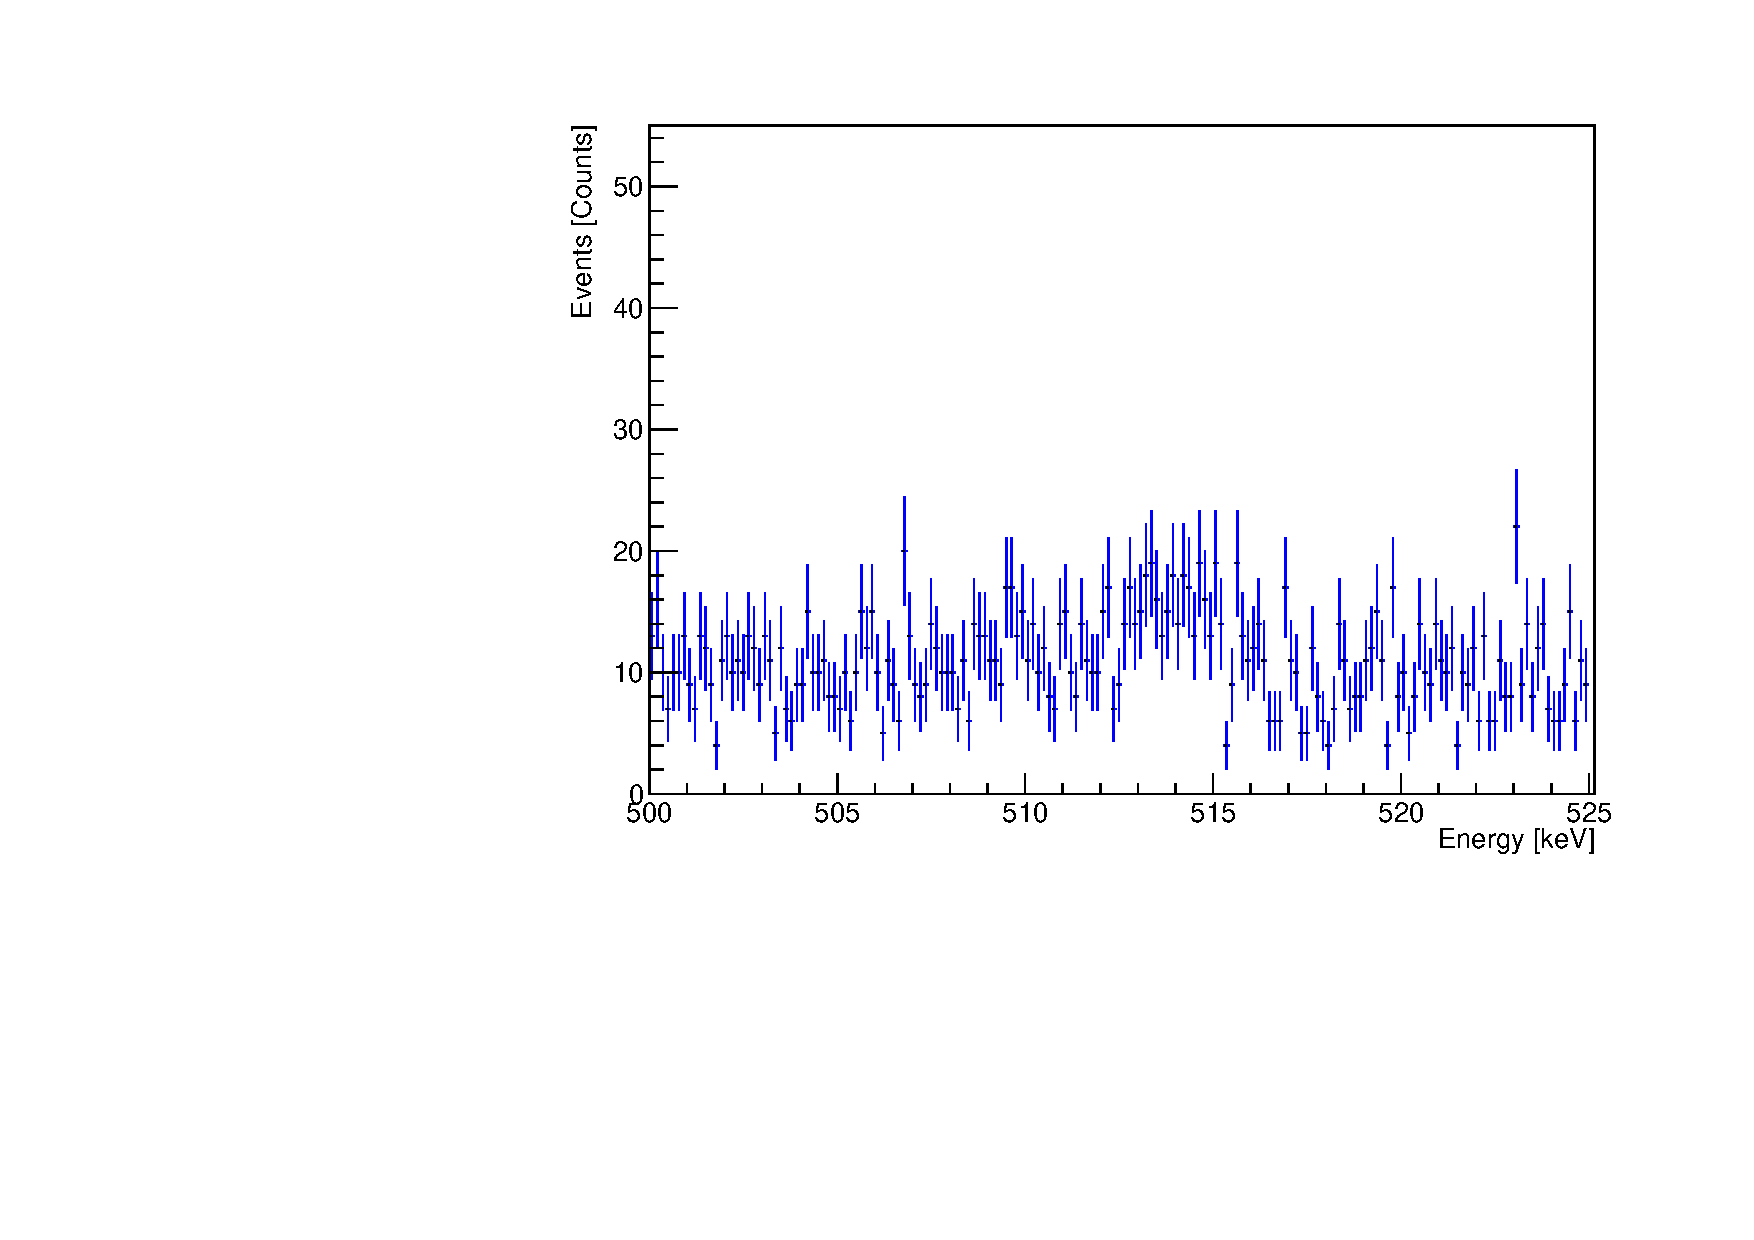
\includegraphics[width=75mm]{./Bilder/500525LArVetoCOAX.pdf}
  \caption{COAX}
  \label{fig:LArCOAX}
\end{subfigure}
    \caption{
    Energy spectra after standard \gerda\ analysis cuts and LAr veto between 500 to 525 keV. 
    The LAr veto made the 511 keV deviation almost completely disappear while the 514 keV deviation is still clearly visible. 
    }
\end{figure}

Due to the occurrence of the 511 keV peak, two different approaches are possible.
One approach would directly apply a double Gaussian peak fit function to the spectra also fitting the 511 keV peak.
Another approach would try to suppress the 511 keV peak and fit a single peak function through the resulting spectra.
Both approaches will be applied in this thesis.
\\

A promising candidate in order to suppress the peak, is the LAr veto.
It is triggered in the case an event in the germanium detectors coincides with a scintillation signal of at least ~0.5 phe \cite{agostini_background_2017}.
The \Kr\ decay into the excited \nuc{Rb}{85m} leaves the escaping electron with a maximum of 173 keV which should only create a very weak scintillation light signal.
Any process involving positron annihilation, however, should create a measurable scintillation light signal visible to the LAr veto setup.
Therefore, the LAr veto should be able to discriminate between \Kr\ gamma events and annihilating events.
\\

Figures \ref{fig:LArBEGes} and \ref{fig:LArCOAX} show the energy spectra after the LAr veto.
One can see that the annihilation peak is reduced compared to the spectra before the LAr veto.
\\

\begin{figure}[t!]
	\centering
	\begin{subfigure}{.5\textwidth}
		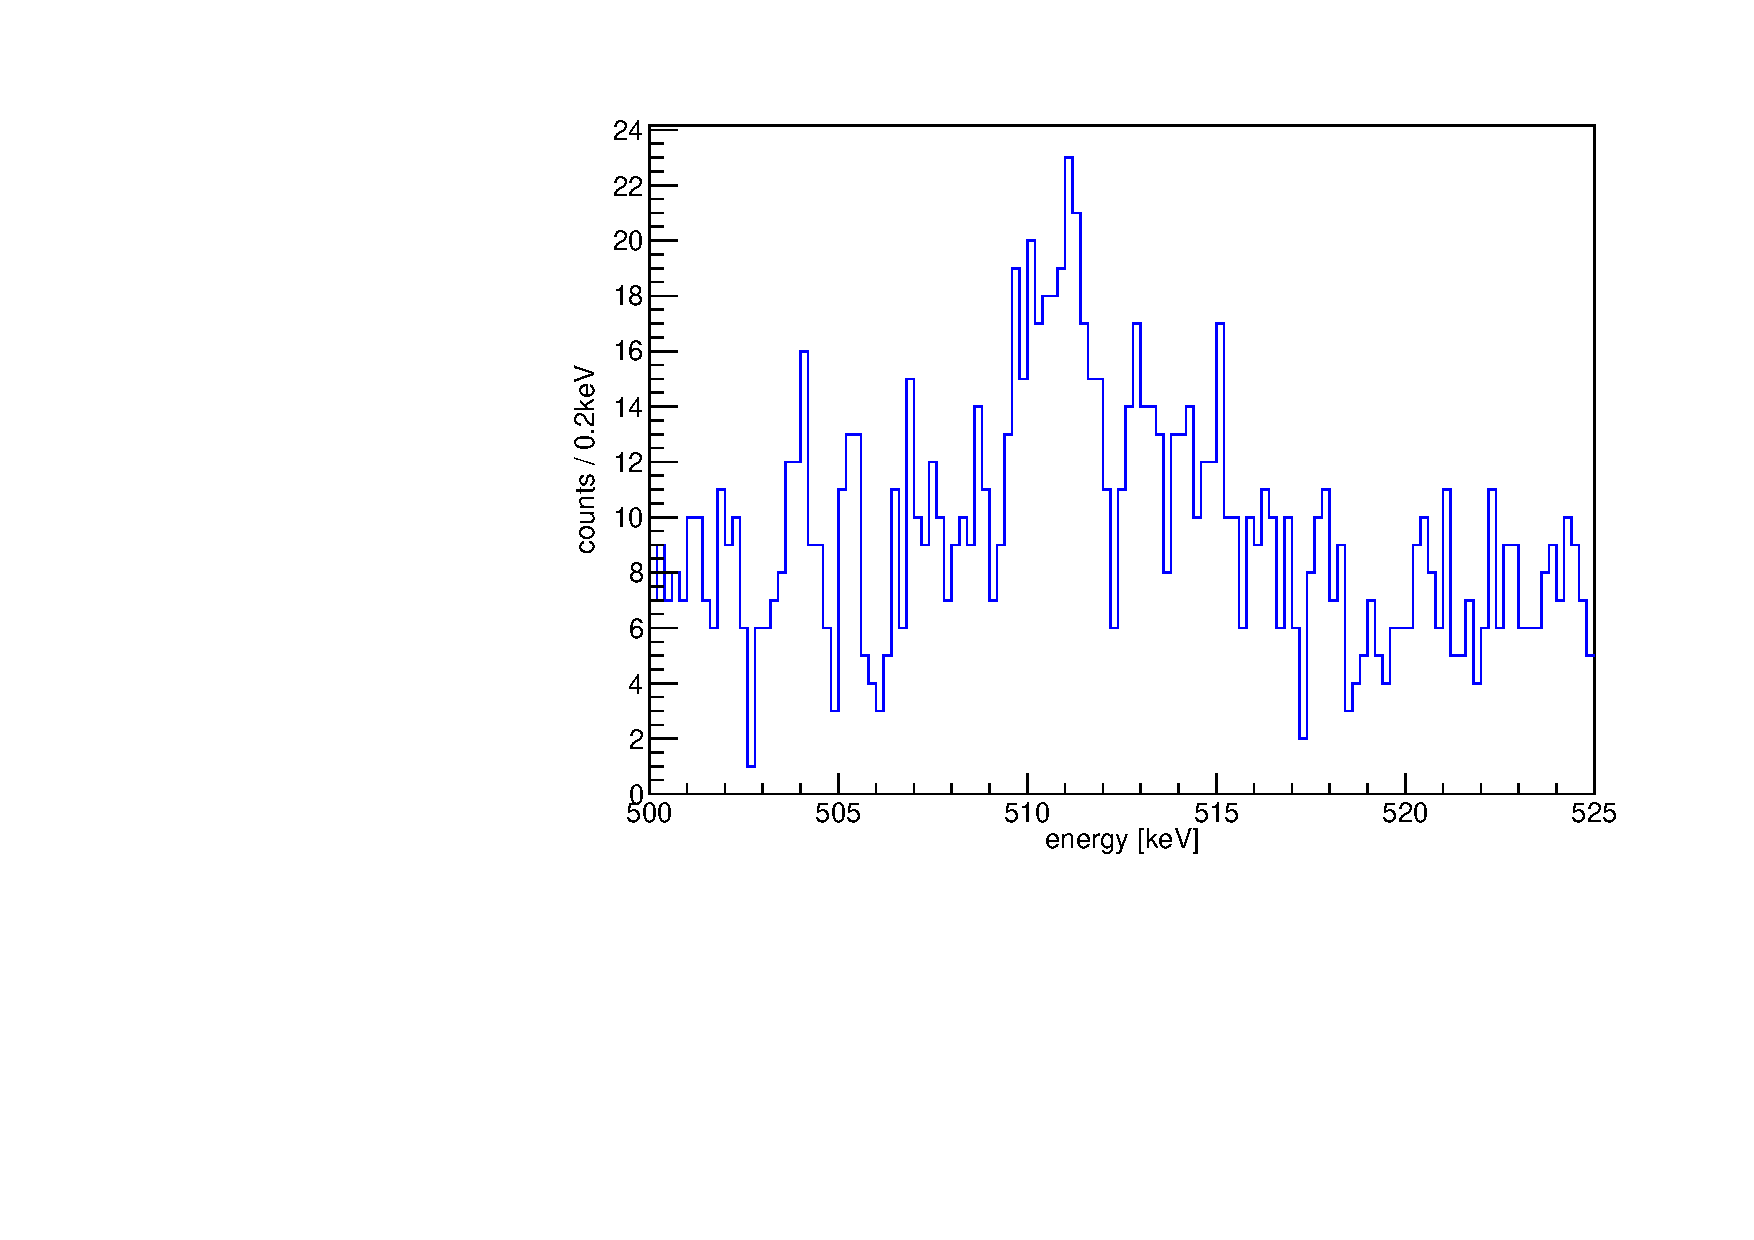
\includegraphics[width=75mm]{./Bilder/AntiLArBEGe.pdf}
		\caption{BEGes}
		\label{fig:AntiLArBEGes}
	\end{subfigure}\hfill%
	\begin{subfigure}{.5\textwidth}
		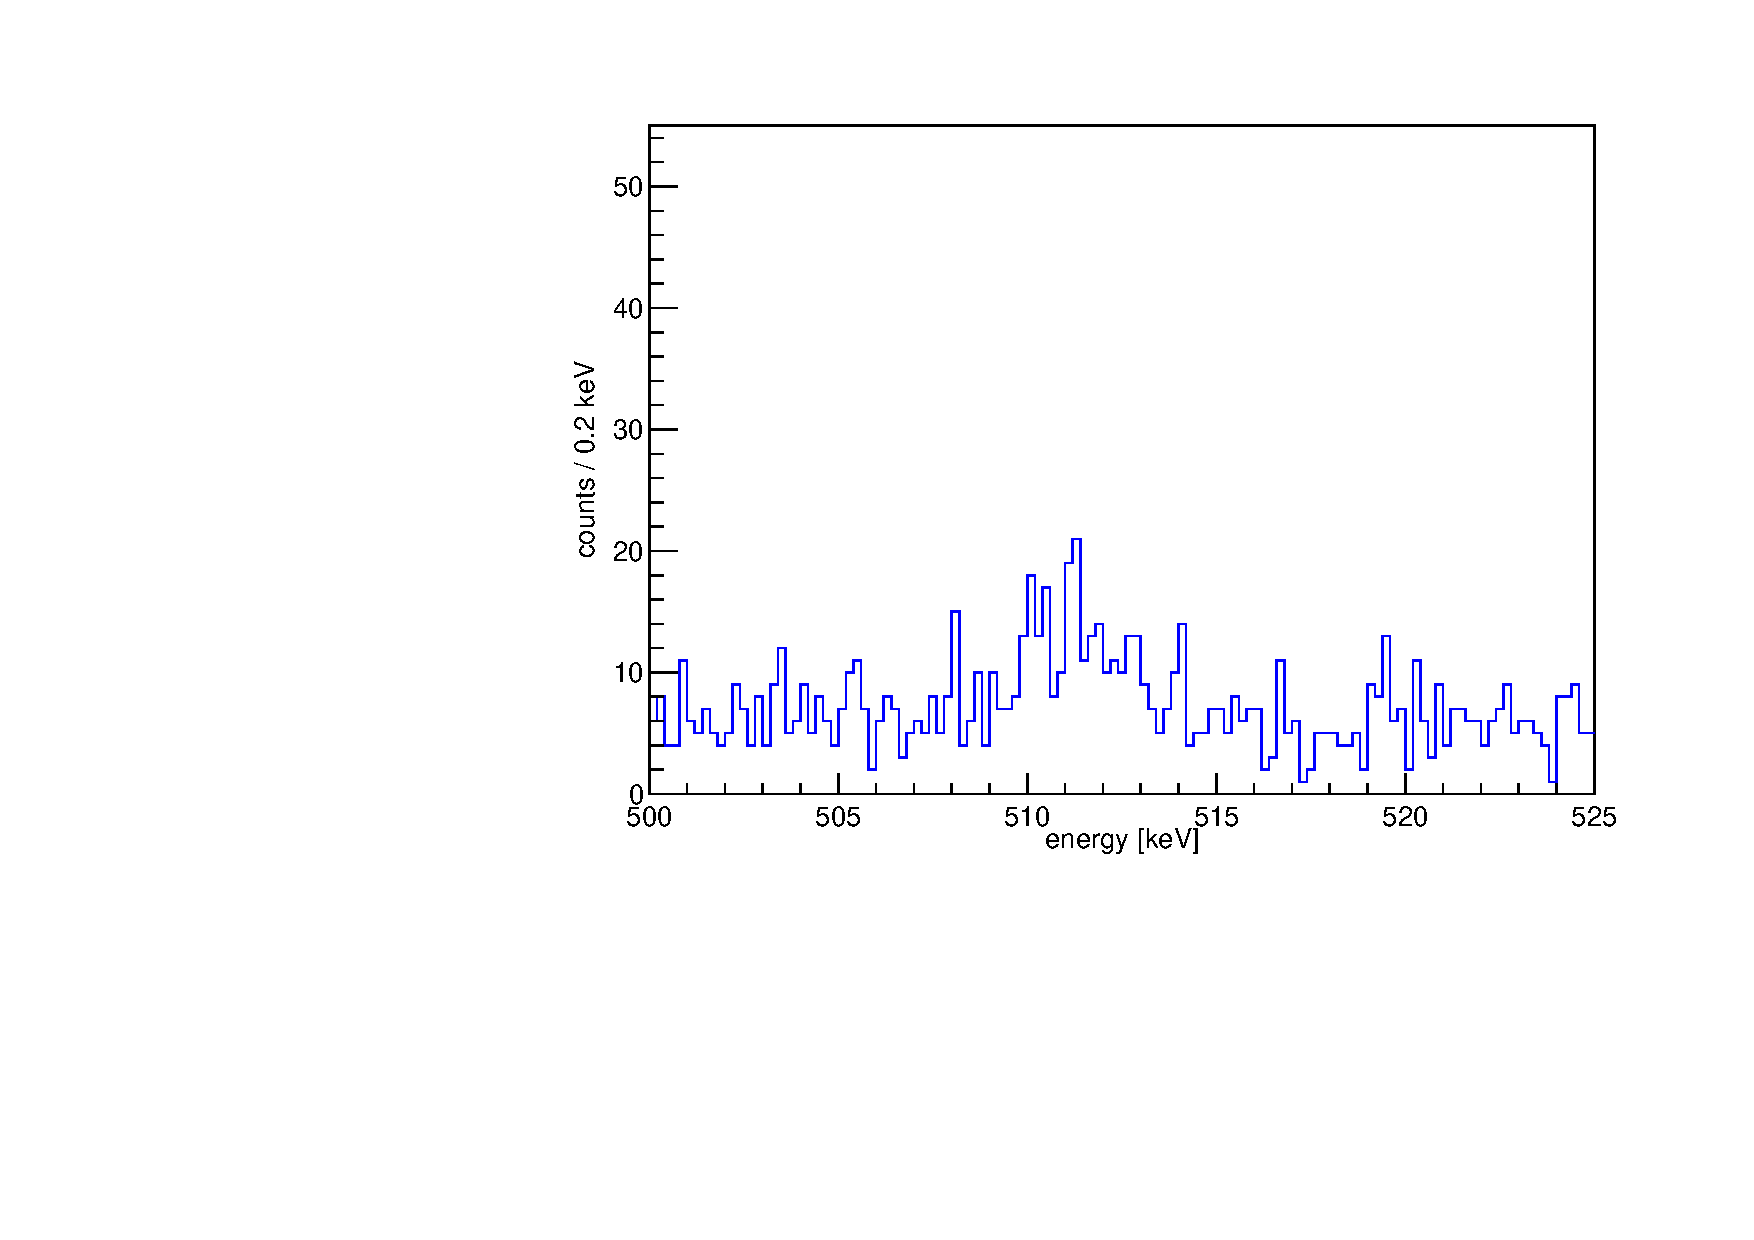
\includegraphics[width=75mm]{./Bilder/AntiLArCOAX.pdf}
		\caption{COAX}
		\label{fig:AntiLArCOAX}
	\end{subfigure}
	\\
	\vspace{0.5cm}
	\caption{
	Energy spectra showing all events previously rejected by the LAr veto between 500 to 525 keV.
	The majority of rejected events lie around the 511 keV mark while also a small deviation around the 514 keV mark can be seen.
	}
\end{figure}

In order to have a better visualization which events have been rejected, all events that triggered the LAr veto are plotted in figures \ref{fig:AntiLArBEGes} and \ref{fig:AntiLArCOAX}.
You can see that the majority of the filtered events had an energy around the 511 keV mark.
\\

Another way to possibly single out the \Kr\ decay caused events would be to look for pre-coincidence events in the LAr setup.
As the excited \nuc{Rb}{85} nuclei has a half life of 1.015 $\mu$s, the scintillation light created by the released beta electron is very probable to be measured before the standard veto time frame looking for a coincidental light signal.
It should therefore be possible to distinguish \Kr\ decays from other events if one is able to find these incidents.
\\


\begin{figure}[t!]
	\centering
	\ifmakefigures%
	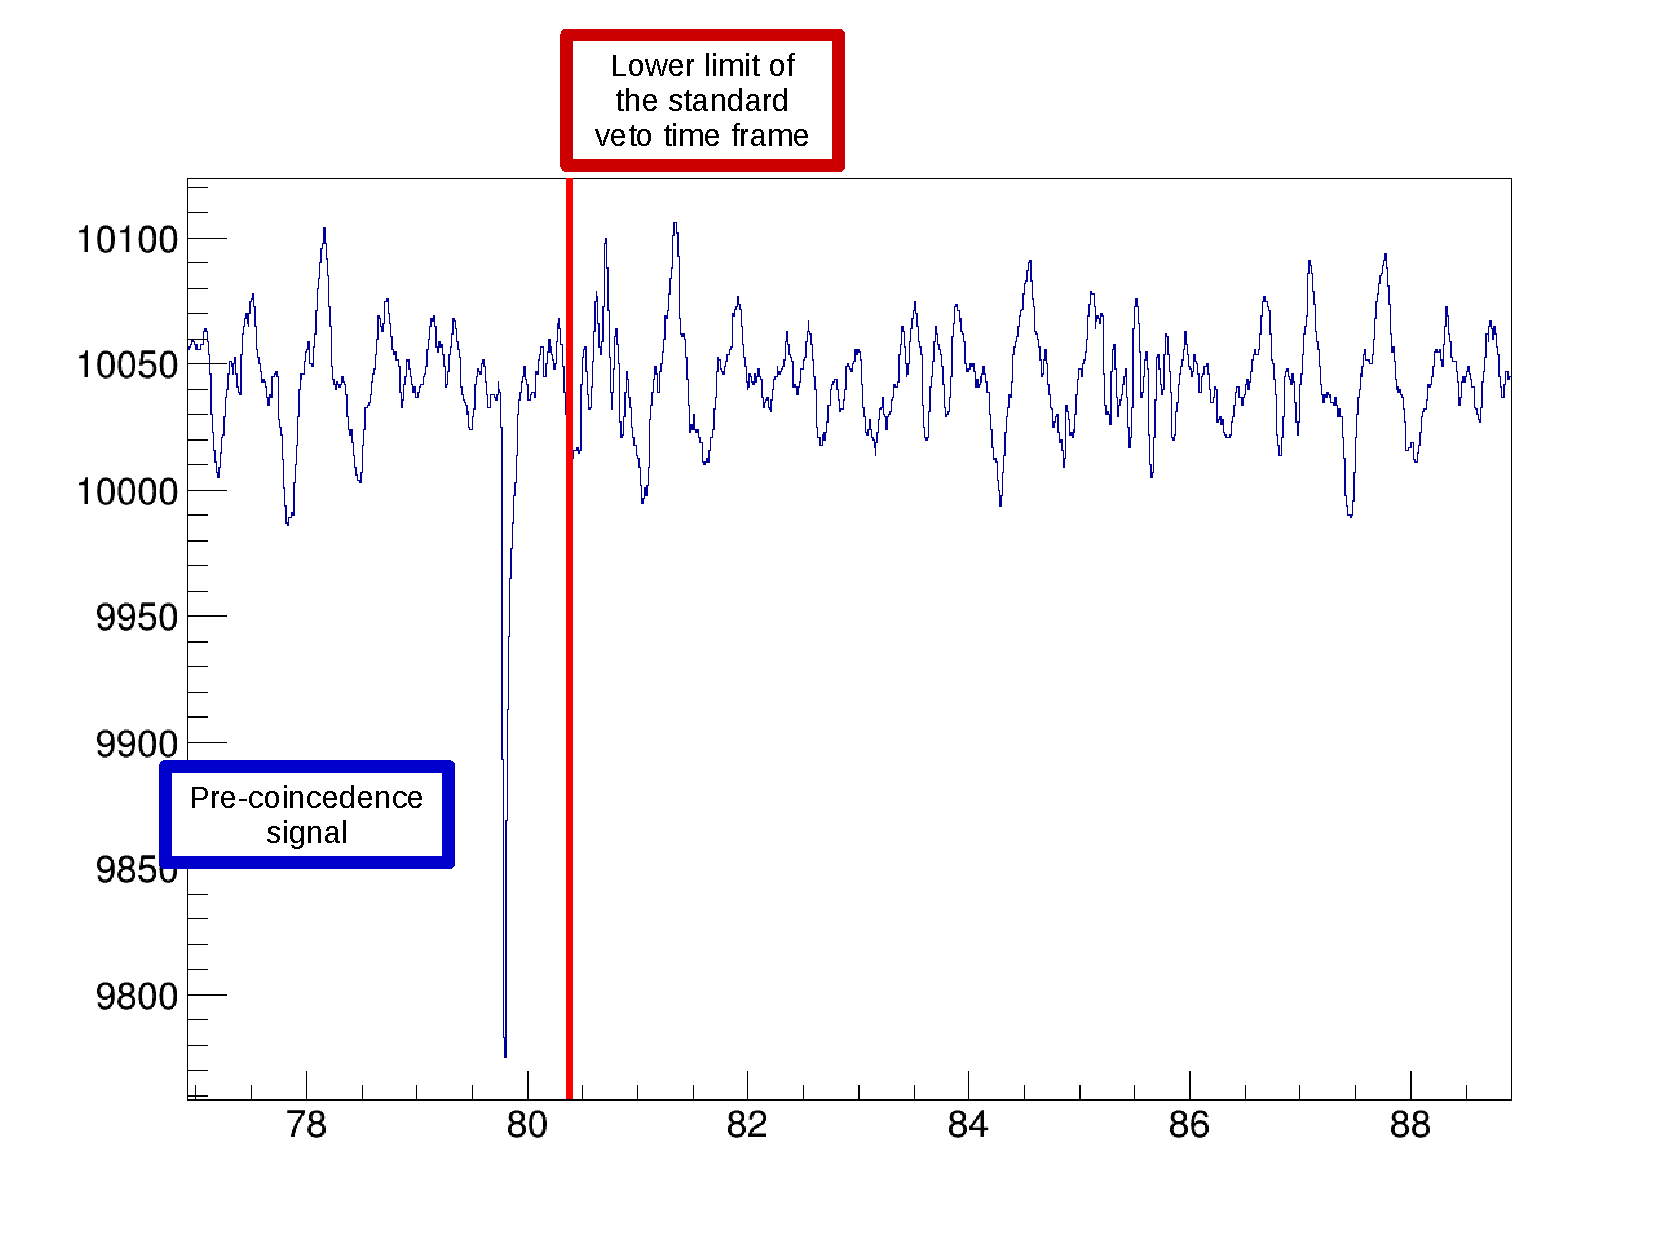
\includegraphics[width=100mm]{./Bilder/Beispiel.pdf}
	\fi%

	\caption{
    The raw signal of photomultiplier tube P4 in event 1614036. 
    The red line shows the lower time window limit for the LAr veto.
    The pulse which has occurred before the time limit, is probably a pre-coincidence event of a \Kr\ decay via the excited \nuc{Rb}{85m} state.
    }
    	\label{fig:BeispielSignal}
    			\vspace{5mm}
\end{figure}


An investigation to find out whether the pre-coincidence signals are usable was applied by plotting all raw measured LAr veto signals of events with an energy around the 514 keV peak and by manually search for any pre-coincidences.
The expected signatures consist of a single peak in the PMTs (for example as seen in figure \ref{fig:BeispielSignal}) or a rising edge in the SiPMs respectively.
However, this investigation showed that almost none of the events considered had any kind of indication for pre-coincidences.
This excludes the presented approach as being a useful \Kr\ indicator.

\iffalse

\fi

\section{Fitting}
\label{sec:Fitting}

The spectra from before and after the LAr veto can now be fitted and, from the fit parameters, the amount of measured \Kr\ decay events determined.
\\

The spectra before the LAr vetoes show two peaks in the investigated area.
This requires the fit function to include two Gaussian functions from which only the parameters of the second peak will be used for further analysis.
In addition to the two Gaussian peaks, a constant background parameter will be added.
Theoretically, the \nuc{Ge}{76} spectra creating this background changes with energy.
In the investigated area, however, its overall change is so small that it can be approximated as constant. 
The resulting fit function is displayed in equation \ref{equ:FitNoFilters}.
\begin{equation}
\mathrm{f}(x) = \mathrm{A}\frac{1}{\sqrt{2\pi}\mathrm{C}}\exp\left(-\frac{(x-\mathrm{B})^2}{2\mathrm{C}^2}\right) + \mathrm{D}\frac{1}{\sqrt{2\pi}\mathrm{C}}\exp\left(-\frac{(x-\mathrm{E})^2}{2\mathrm{C}^2}\right) + \mathrm{F}
\label{equ:FitNoFilters}
\end{equation}
Figures \ref{fig:FitNoFilterBEGes} and \ref{fig:FitNoFilterCOAX} show the resulting fitting plots.
The values of the fit parameter values can be seen in the table inside the figures.
Fitting parameters B and E - the mean values of the peaks - were fixed to the values of 511 keV and 514 keV respectively.
All other values were left free under the condition of a positive value.
Also, parameter C - the sigma value - was used for both peaks.
In the energy area investigated, the two resolutions and thus also the variances at the specific energies should not vary greatly, which is why this simplification can be applied.
The previously determined resolutions can be used to calculate the expected values for the variances, as shown in appendix chapter \ref{sec:ResDetermination}: $\sigma_{\mathrm{BEGe}} = 0.96 \ \unit{keV}$ for the BEGe detectors and $\sigma_{\mathrm{COAX}} = 1.16 \ \unit{keV}$ for the COAX detectors.
The values determined in the fitting process have the corresponding expected value in their range of uncertainty .
\\

\begin{figure}[t!]
	\centering
	\begin{subfigure}{.5\textwidth}
		\centering
		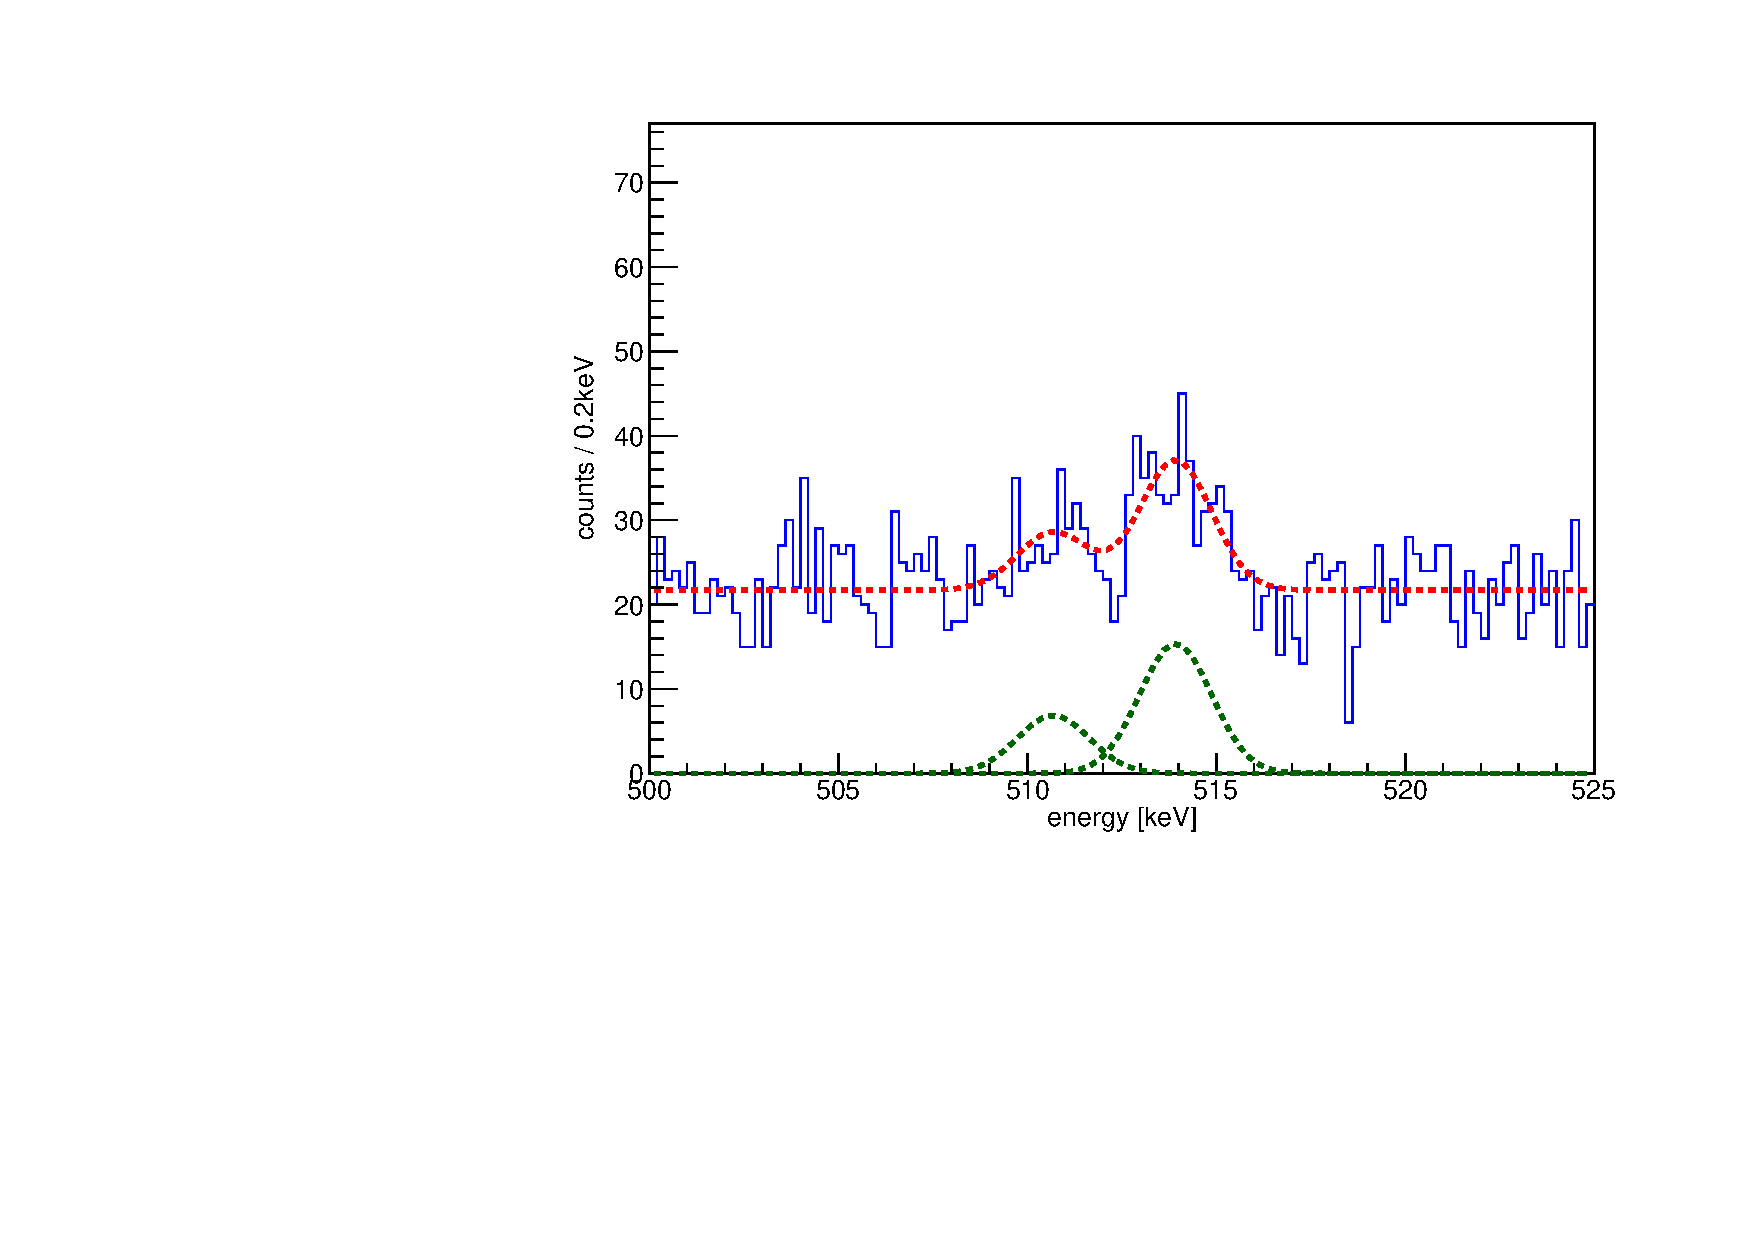
\includegraphics[width=\textwidth]{./Bilder/500525FitNoFilterBEGes.pdf}
		\caption{BEGes}
		\label{fig:FitNoFilterBEGes}
	\end{subfigure}\hfill%
	\begin{subfigure}{.5\textwidth}
		\centering
		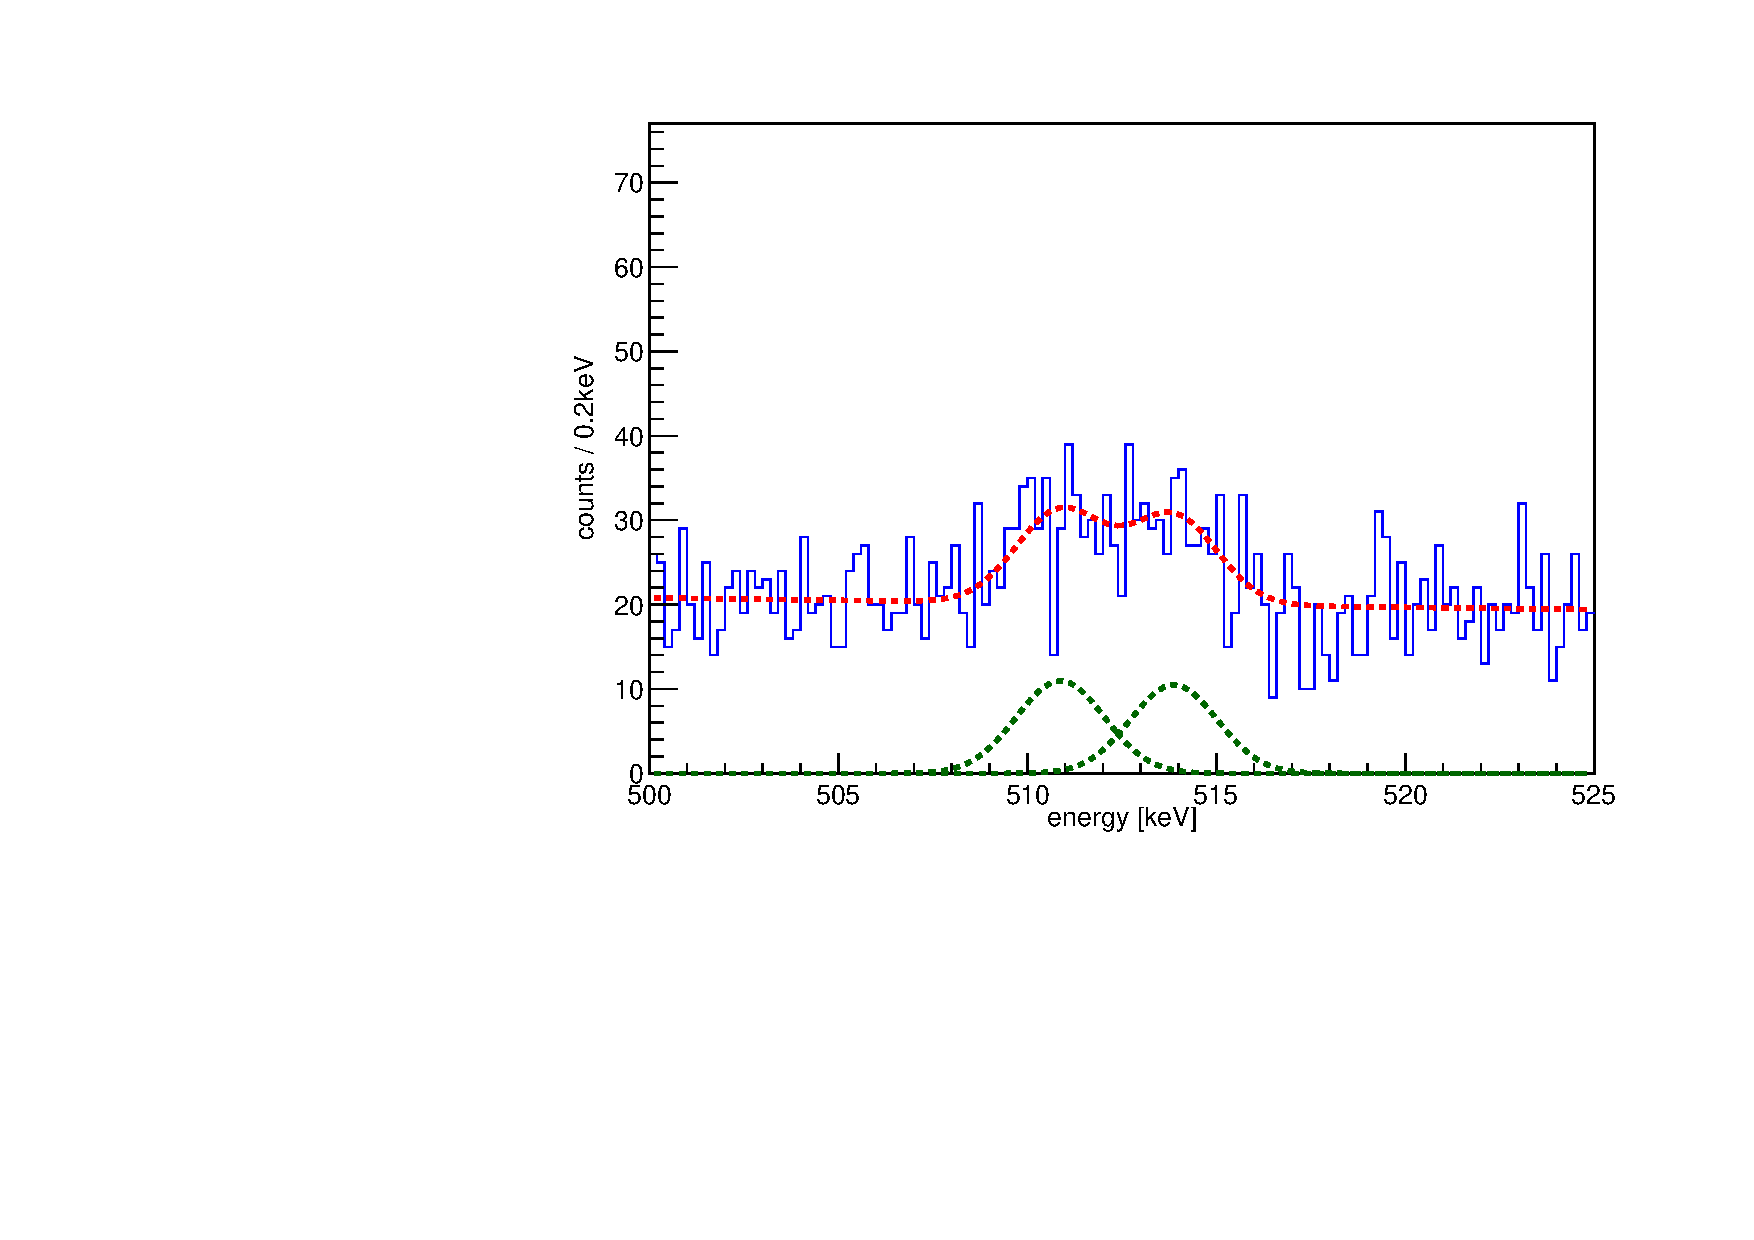
\includegraphics[width=\textwidth]{./Bilder/500525FitNoFilterCOAX.pdf}
		\caption{COAX}
		\label{fig:FitNoFilterCOAX}
	\end{subfigure}
    \\
	\caption{
		Fitted energy spectra before the LAr veto cut between 500 and 525 keV. 
		Function \ref{equ:FitNoFilters} was used as fit function and its course is indicated in red. 
		The two green plots at the bottom of the figures indicate the two independent peaks. 
		}
\end{figure}
\\

\iffalse

\begin{table}[t!]
\centering
\begin{tabular}{|l|c|c|}
\hline
Name	& Value [BEGe] & Values [COAX]\\ 
\hline
A [counts $\times$ / 0.2 ] &	(15.98 \(\pm\)	4.54)&	(31.93\(\pm\)7.08)	\\	
\hline
B [keV] &	(510.87 \(\pm\)	0.22)&	(510.88 \(\pm\)	0.190)\\	
\hline
C [keV] &	(0.952 \(\pm\)	0.011)	&	(1.165 \(\pm\)	0.010)	\\
\hline
D [counts / 0.2 keV] &	(36.66 \(\pm\)	4.99)	&	(30.40 \(\pm\)	5.24)	\\
\hline
E [keV] &	(513.95 \(\pm\)	0.16)	&	(513.87 \(\pm\)	0.14)	\\
\hline
F [keV] &	(0.953 \(\pm\)	0.014)	&	(1.145 \(\pm\)	0.012)	\\
\hline
G [counts / 0.2 keV] &	(11.98 \(\pm\)	5.27)	&	(11.35 \(\pm\)	7.45)	\\
\hline
H [counts / 0.2 keV] &	(189.92 \(\pm\)	110.05)	&	(996.72 \(\pm\)	972.62)	\\
\hline
I [1/keV] &	(5.80 \(\pm\) 1.22)$\times10^{-3}$	&	(9.24 \(\pm\)1.83)$\times10^{-3}$ \\
\hline

\end{tabular}
\caption{
	Fit parameters of fit function \ref{equ:FitNoFilters} applied on the spectra of the respective detectors. 
	Variable A and D correspond to the amplitudes of the two Gaussian peaks, B and E to the position of their maxima, C and F their standard deviation. 
	On the other hand is G the constant background, H the amplitude of the exponential background and I its decrease parameter.
	}
\label{tab:FitParNoFilter}
\end{table}
\\
\fi

However, the only fit parameter of real interest in this case is variable D.
Its value is the amplitude of the second Gaussian peak.
As the Gaussian peak function was already chosen in the normalized form, this value also represents the amount of \Kr\ decays.
Taking into account the binning of the histograms, a value of  
\begin{equation*}
N_{\mathrm{peak,BEGe}} = (183\pm25) \ \unit{cts}
\end{equation*} 
in the peak of the BEGe spectrum and
\begin{equation*}
N_{\mathrm{peak,COAX}} = (152\pm26) \ \unit{cts}
\end{equation*}
in the COAX spectrum has been detected.
\\

When it comes to the spectrum after the LAr veto, fit function \ref{equ:FitNoFilters} will also be used again.
This is an advantage because it will also fit around a possible remaining 511 keV peak which otherwise might have affected the outcome.
Diagrams \ref{fig:FitLArVetoBEGes} and \ref{fig:FitLArVetoCOAX} show the fitted plots.
Like above, the amplitude D of the second Gaussian peak corresponds to the number of events measured in the area of the peak per binning.
This results in an amount of $(120\pm19)$ counts for the BEGe and $(128\pm22)$ for the COAX spectrum.
\\

Compared to the values of the non LAr filtered spectra, however, it can be seen that the number of counts in the BEGe and in the COAX detectors have dropped considerably.
This means that the LAr veto also rejected some of the \Kr\ decay caused events.
Therefore only the results of the spectra before the LAr veto can be used for the further analysis.
\\



\begin{figure}[t!]
	\centering
	\begin{subfigure}{.5\textwidth}
		\centering
		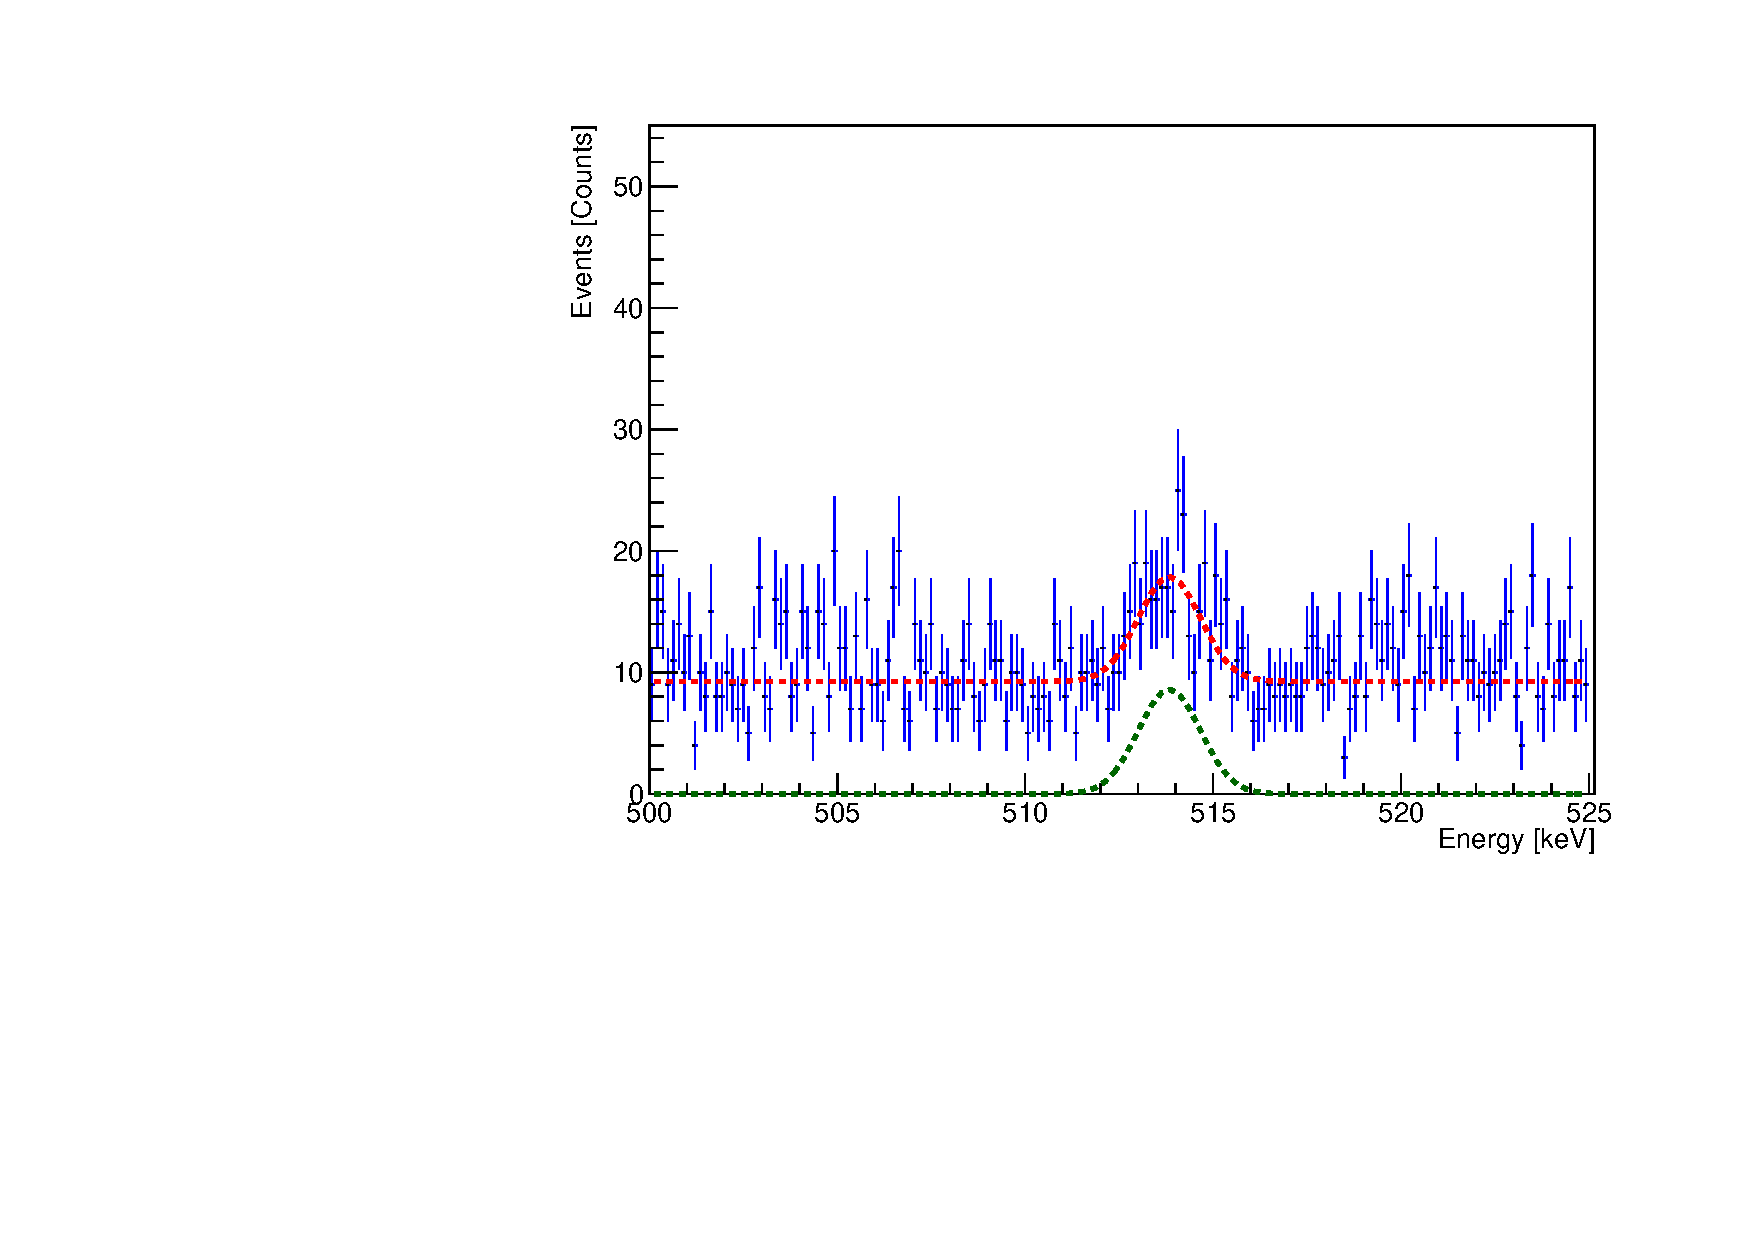
\includegraphics[width=\textwidth]{./Bilder/500525FitLArVetoBEGes.pdf}
		\caption{BEGes}
		\label{fig:FitLArVetoBEGes}
	\end{subfigure}\hfill%
	\begin{subfigure}{.5\textwidth}
		\centering
		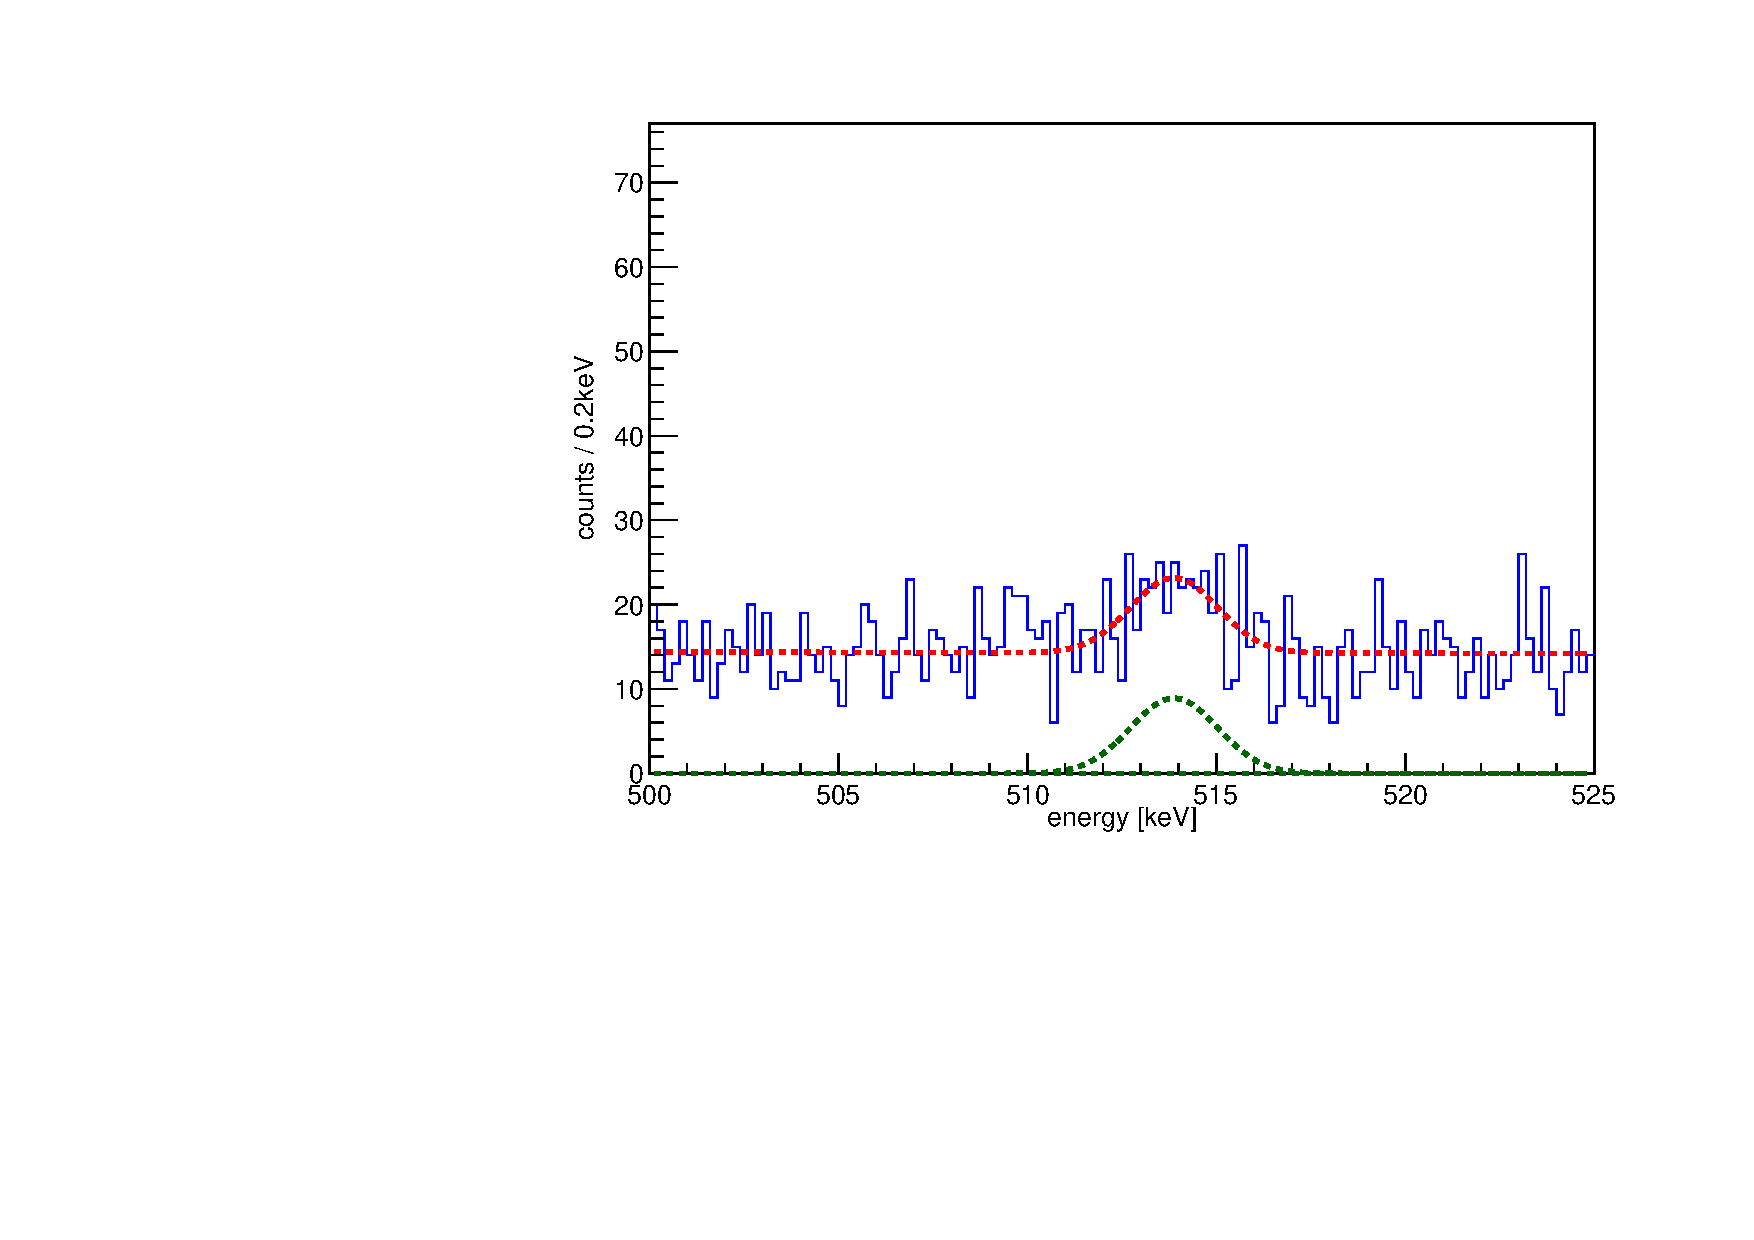
\includegraphics[width=\textwidth]{./Bilder/500525FitLArVetoCOAX.pdf}
		\caption{COAX}
		\label{fig:FitLArVetoCOAX}
	\end{subfigure}
	\caption{
	Fitted energy spectra after the LAr veto between 500 and 525 keV. 
	Function \ref{equ:FitNoFilters} was used as fit function again. 
    In the case of the BEGe spectrum, the first peak function vanishes due to no measurable deviation from the background level at the 511 keV mark.
    In the COAX spectrum, however, a deviation is still visible which is why the second peak function has a finite amplitude.
	}
\end{figure}
\iffalse
\begin{table}[t!]
	\centering
	\begin{tabular}{|l|c|c|}
		\hline
		Name	& Value [BEGes] & Value [COAX]\\ 
		\hline
		A [counts  / 0.2 ] &	(24.094734$\pm$3.856334)&	(25.680418$\pm$4.424006)\\	
		\hline
		B [keV] &	(513.925781$\pm$0.129591)&	(513.884766$\pm$0.185506)\\	
		\hline
		C [keV] &	(0.952731$\pm$0.019180)	&	(1.145909$\pm$0.018075)\\
		\hline
		D [counts / 0.2 keV] &	(14.548210$\pm$0.349083)	&	(10.602730$\pm$8.090884)\\
		\hline
		E [counts / 0.2 keV] &	(0.607414$\pm$5.193491)	&	(10.000000$\pm$9.831094)\\
		\hline	
		F [1 / keV] &	(0.901209$\pm$2.409593)	&	(0.001950$\pm$0.004637)\\
		\hline
	\end{tabular}
	\caption{
		Fit parameters of fit function \ref{equ:FitNoFilters} applied on the spectra of the respective detectors. 
		Variable A correspond to the amplitudes of the Gaussian peak, B to the position of its maximum, C its standard deviation. 
		On the other hand is D the constant background, E the amplitude of the exponential background and F its decrease parameter.
		}
			\label{tab:FitParFilter}

\end{table}
\fi

\iffalse
Nevertheless, the line count rate $N_{\mathrm{peak,BEGe}}$ and $N_{\mathrm{peak,COAX}}$ used in the further analysis were successfully determined from the fit of the unfiltered spectra.
These values represent the amount of events that were with almost absolute certainty caused by a 514 keV photon of the \nuc{Rb}{85m} relaxation.  
To be able to calculate the values of actual amount of \Kr\ per liter necessary for this amount of counts to be measured one has to determine a conversion factor. 
How this conversion factor can be determined is the topic of the following section.
\\
\fi

\section{Monte Carlo Simulation}
\label{sec:MonteCarlo514}

It is possible to calculate the decay density of \Kr\ necessary to create the measured line count by using the conversion factor $1/p \epsilon V_{\mathrm{sim}} $ between these two values. 
Such a conversion factor can be determined with the help of a Monte Carlo simulation.
The tool used to perform this simulation is \mage (MAjorana-GErda), a GEANT4-based physics simulation software developed jointly by MAJORANA and \gerda\.
\mage is specialized in the simulation of radioactive decays and their corresponding energy deposition in germanium detectors \cite{boswell_mage_2011}.
In this thesis, the full \gerda\ implementation is used.
\\

A number of $N_{\mathrm{sim}}$ = 50.000.000 gammas with 514 keV were simulated in cylindrical volume of 2.5 m height and a diameter of 3 m resulting in $V_{\mathrm{sim}} = 17.65 \mathrm{m}^3$.
Compared with the volume of 64 m\(^3\) of LAr used in the \gerda\ experiment, this volume is much smaller.
Nevertheless, as we will see later, this volume is by far big enough for this purpose.
\\

\begin{figure}[t!]
	\centering
	\begin{subfigure}{.5\textwidth}
		\centering
		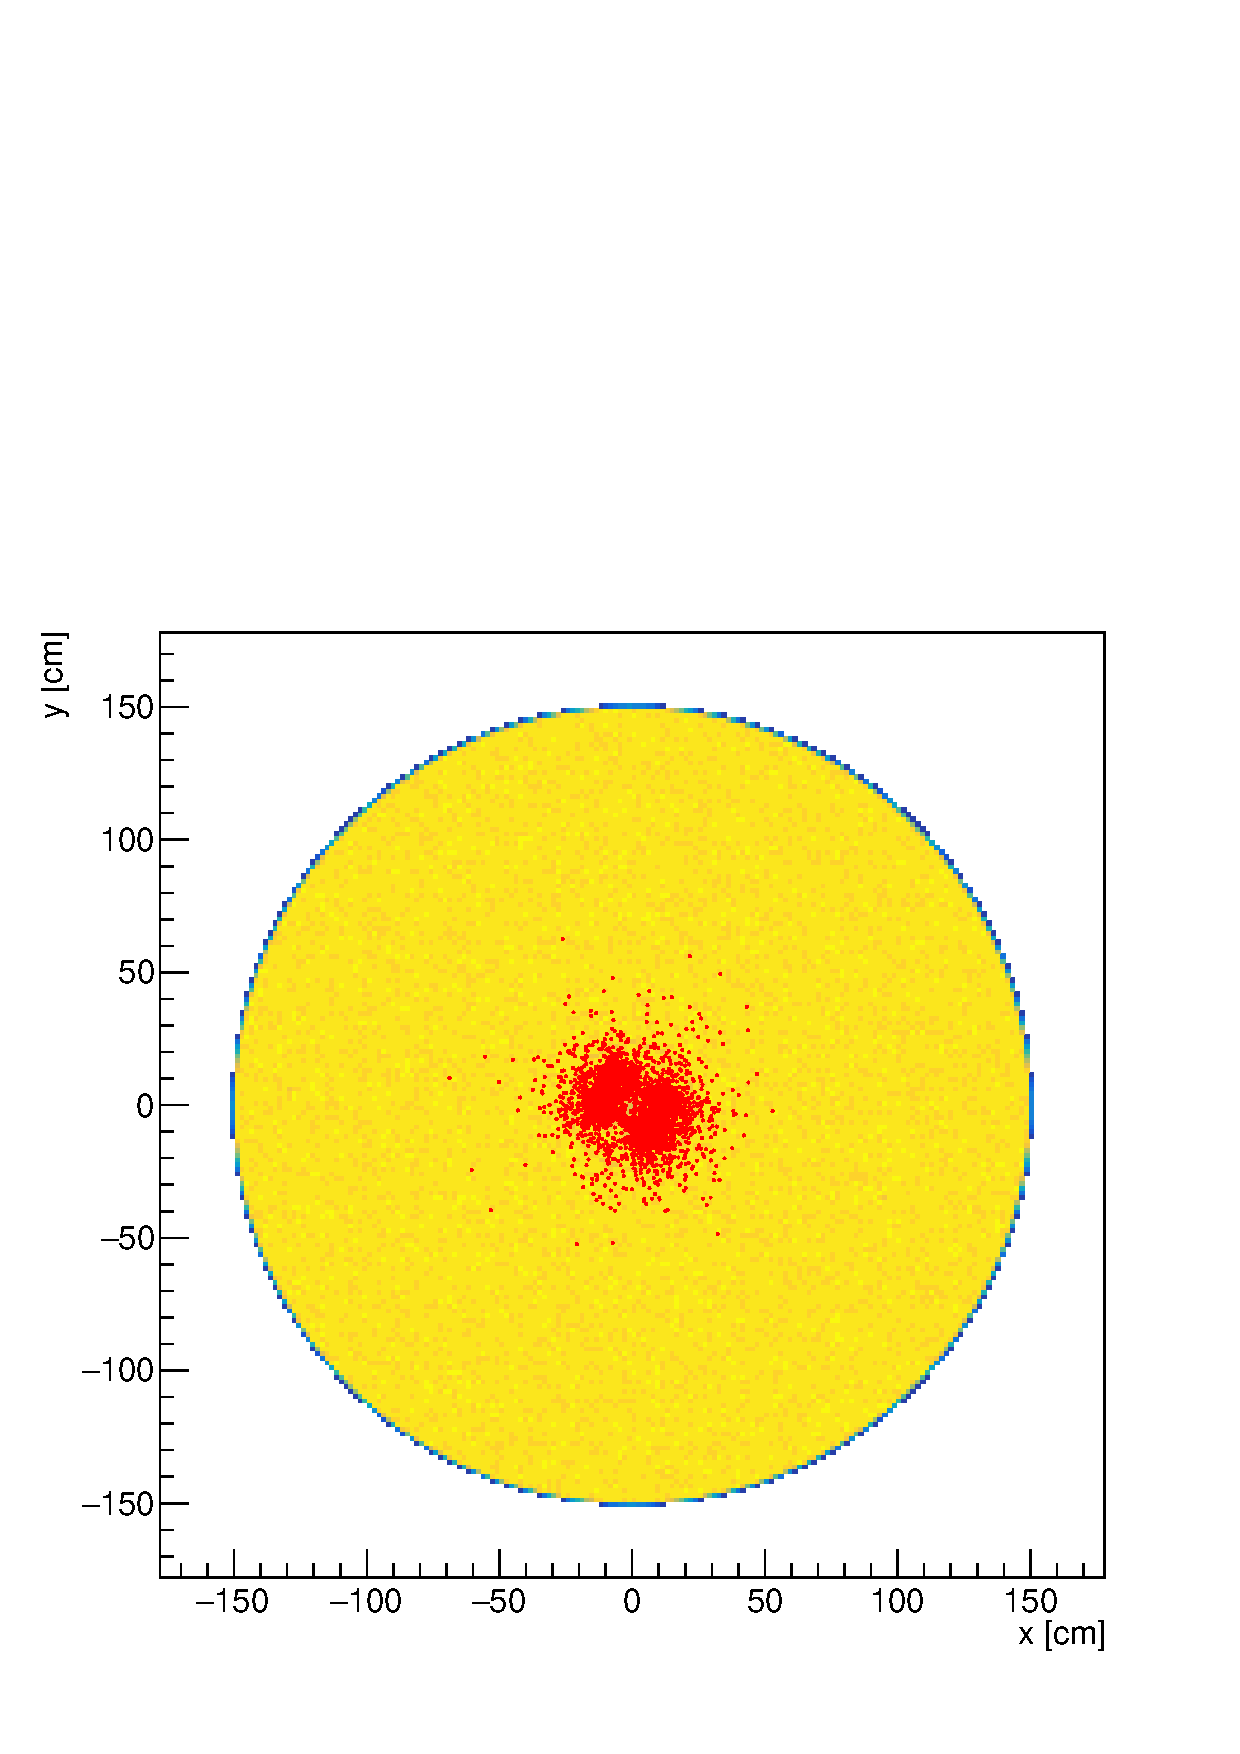
\includegraphics[height=75mm]{./Bilder/MC-Querschnitt-BEGes.pdf}
		\caption{Cross section from above}
		\label{fig:CrossSecAb}
	\end{subfigure}\hfill%
	\begin{subfigure}{.5\textwidth}
		\centering
		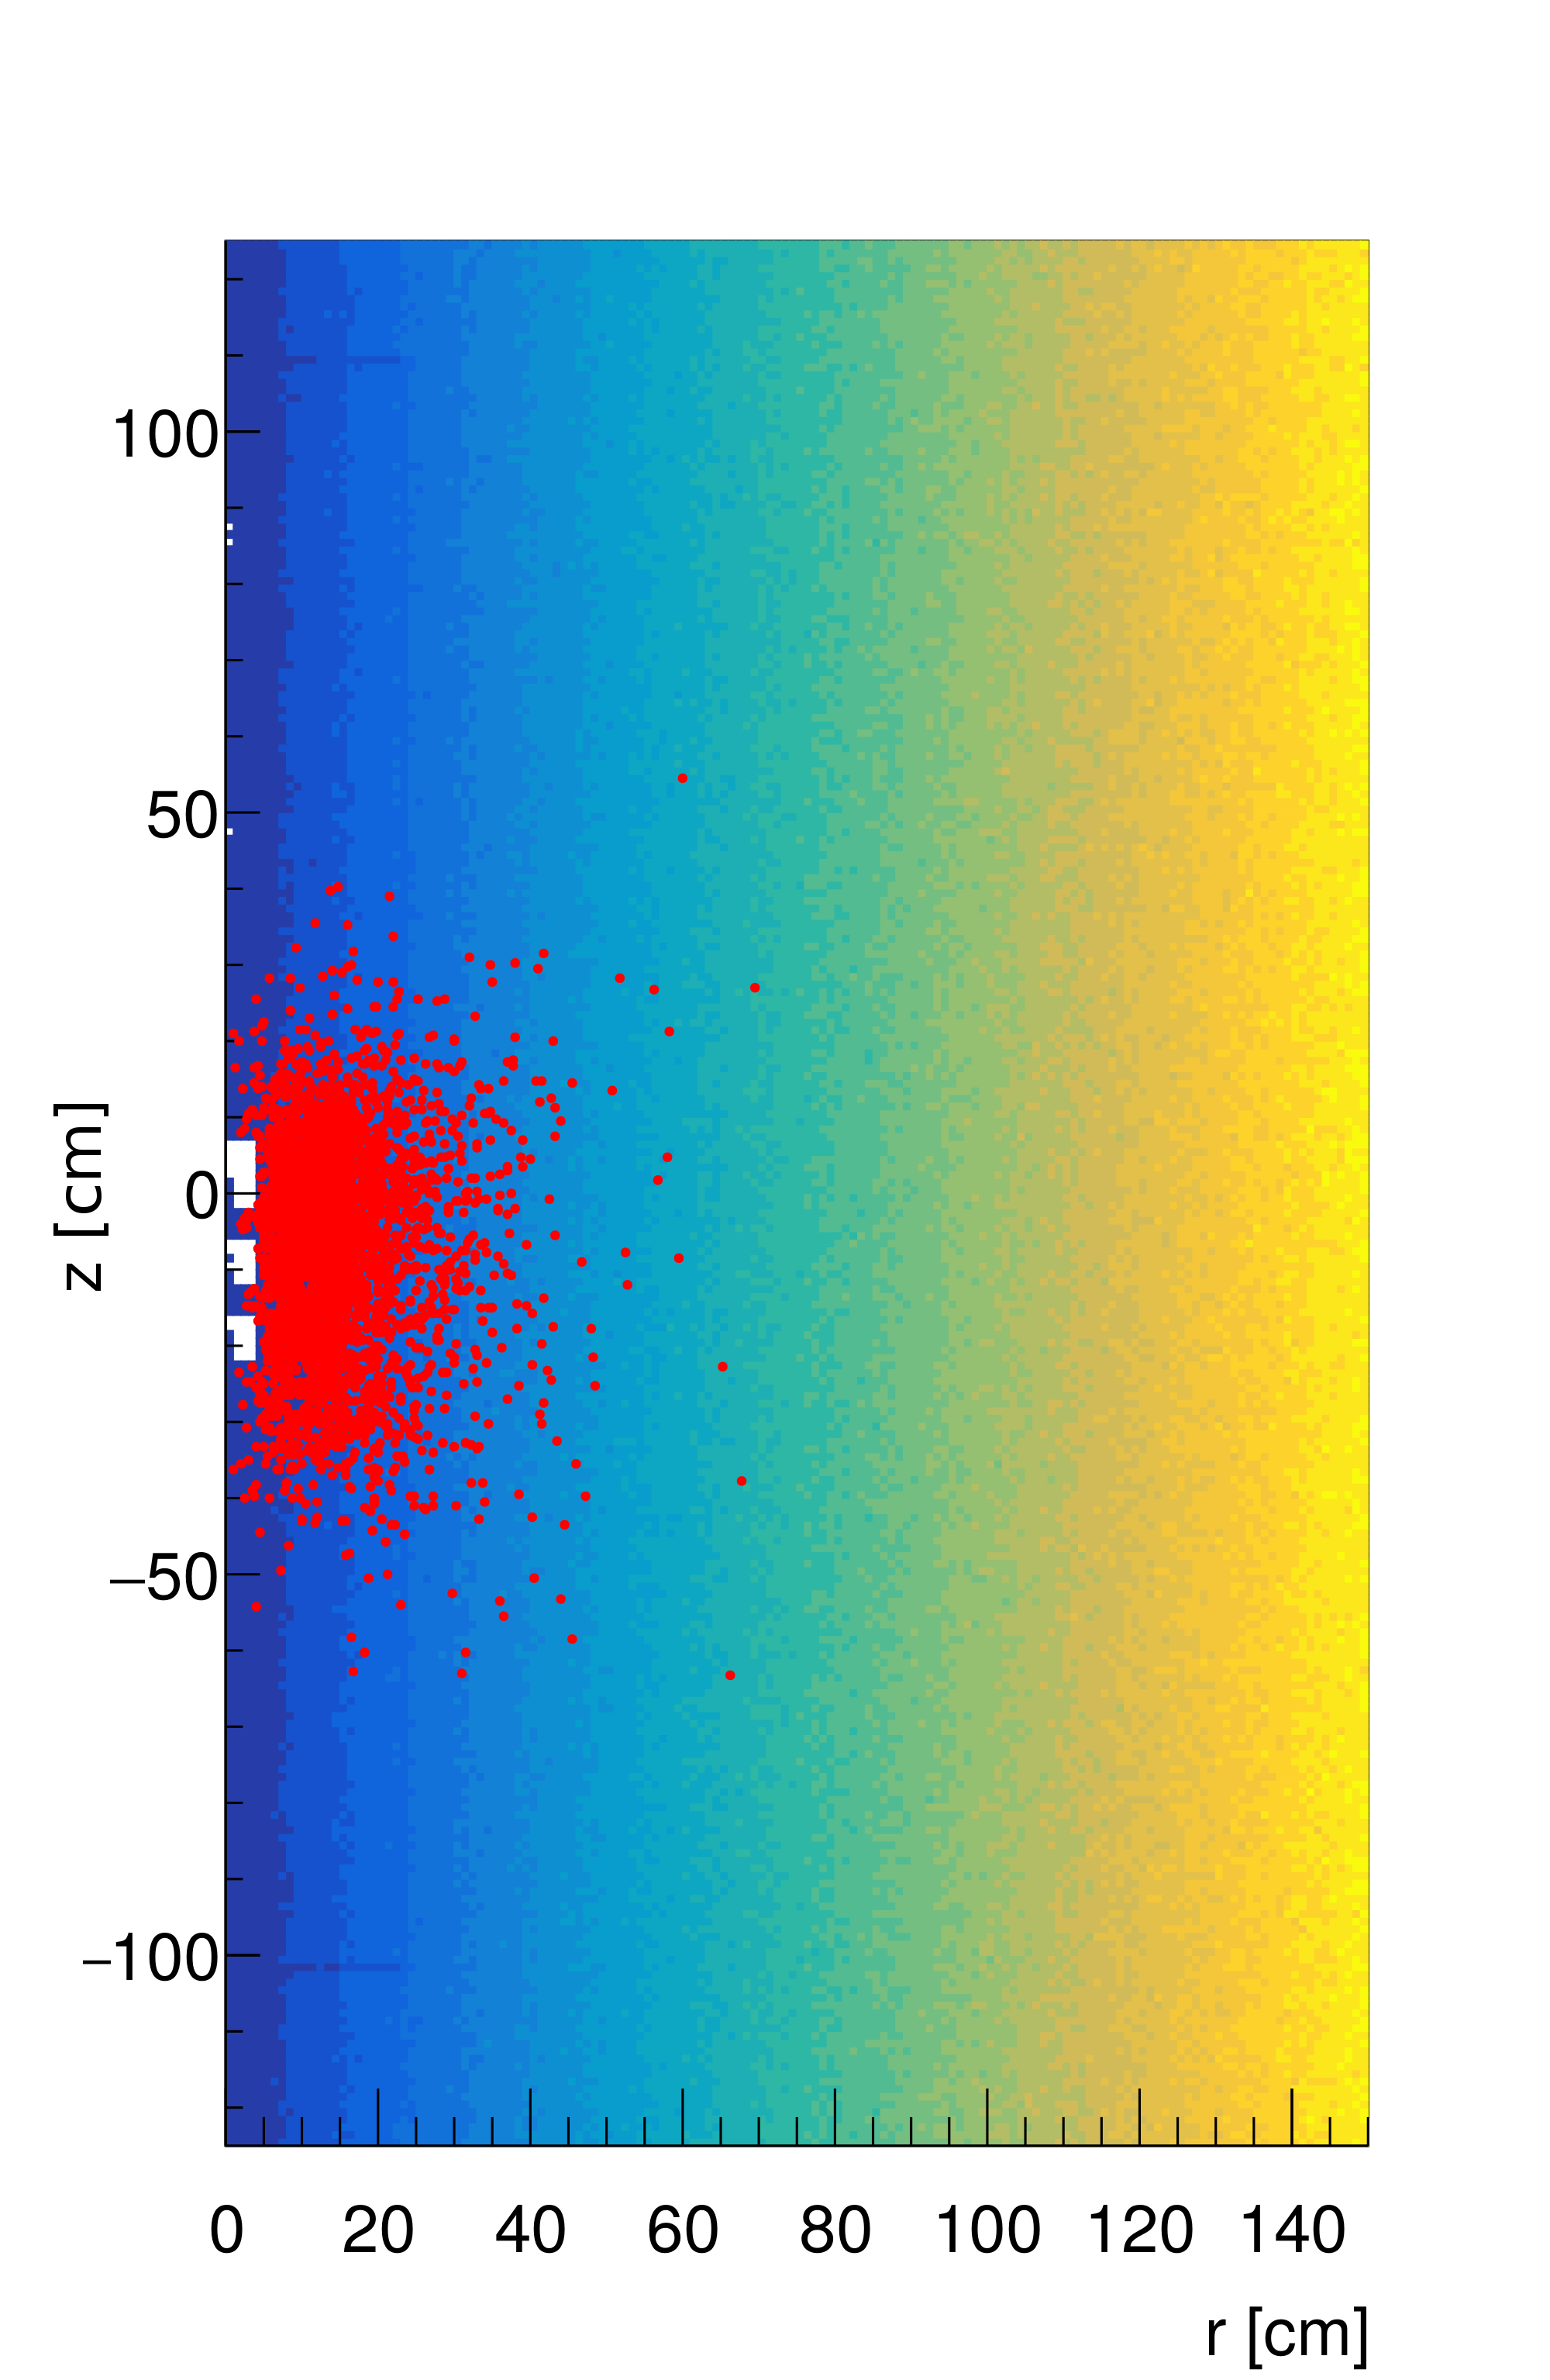
\includegraphics[height=75mm]{./Bilder/MC-Radius-BEGes.png}
		\caption{Radial projection}
		\label{fig:CrossSecRa}
	\end{subfigure}
    \\
	\vspace{0.5cm}
    \caption{
    	The cross section of the simulated volume from above and its radial projection.
    	The colored area shows the density of all simulated decays. 
    	The red points indicate all events that were measured by BEGe detectors.
    	It can be seen that gamma emitted far away from the detectors did not produce a measurable signal in the detectors.
    	}
\vspace{0.5cm}
\end{figure}
\\

\begin{figure}[t!]
	\centering
	\ifmakefigures%
	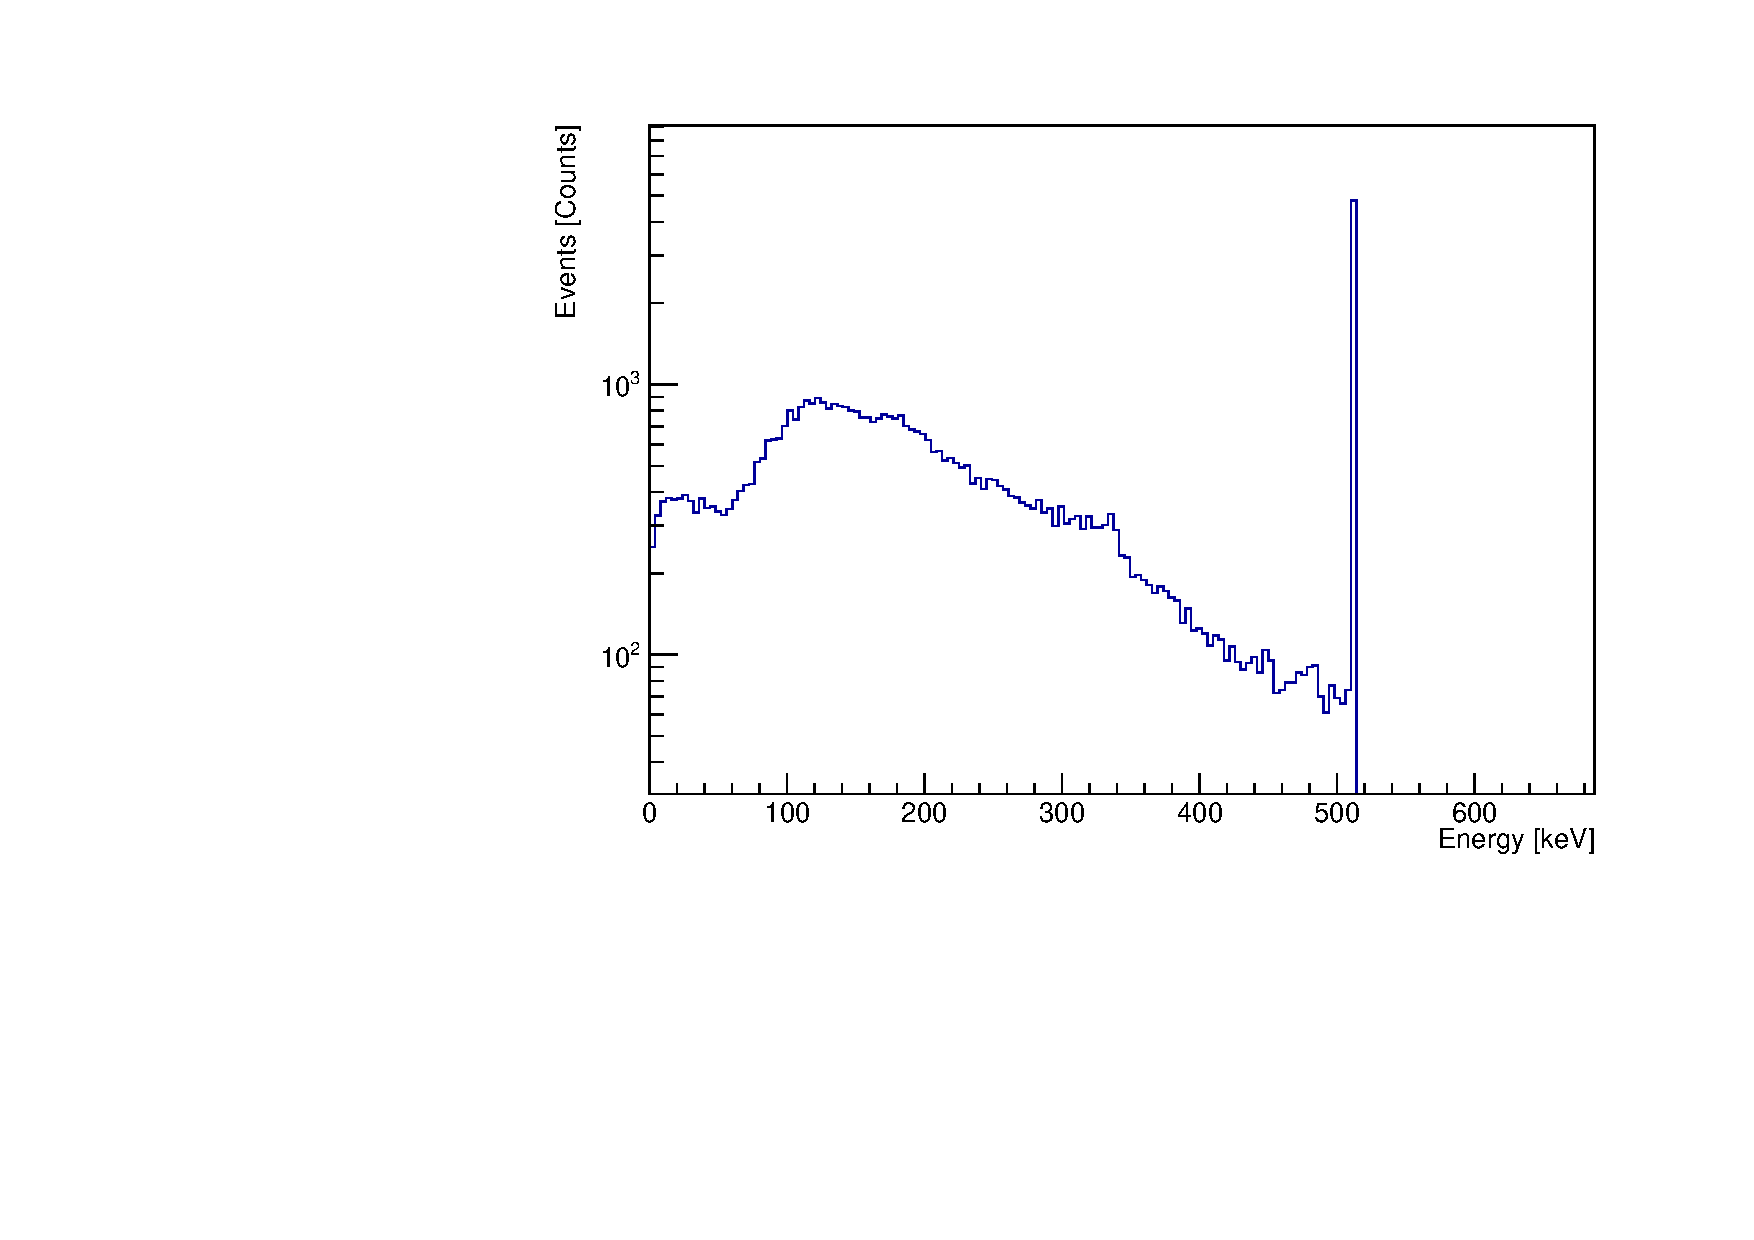
\includegraphics[width=100mm]{./Bilder/MC-514-Phasenraum.pdf}
	\fi%
	\caption{
    Energy spectrum of simulated events measured in BEGe detectors.
	The blue colored bin represents the counts used for determining the detector efficiency.
	The majority of measured signals has an energy below 514 keV.
	Among other things, the Compton peak at roughly 343keV can be seen.  
	}
	\label{fig:PhasenraumMC514}
			%\vspace{5mm}
\end{figure}

From these 50 million simulated gammas with the anti-coincidence veto already applied only about 75 thousand have created a signal in a detector, only 30465 of them in a BEGe and 24902 in a COAX.
The spatial distribution of all measured events in the BEGe detectors can be seen as red dots in figures \ref{fig:CrossSecAb} and \ref{fig:CrossSecRa}.
Furthermore, the spectrum of all events detected in BEGe detectors is shown in Figure \ref{fig:PhasenraumMC514}.
One can see that only in a small number of cases the gamma deposited all of its initial 514 keV in the detectors.
The majority of photons measured must have scattered before they arrived in the detector or did not deposit all their energy in them.
To calculate the detector efficiency, however, only the measured events at the 514 keV peak have to be accounted for.
In the BEGe detector spectrum, the peak contains a total of \(\Delta N_{\mathrm{BEGe}} = (4511\pm67) \) counts while peak contains \(\Delta N_{\mathrm{COAX}} = (3706\pm60) \) in the COAX detectors .
With a total of 50 million initial decays, this results in an efficiency of 
\begin{equation*}
\epsilon_{\mathrm{BEGe}} = \frac{\Delta N_{\mathrm{BEGe}}}{N_{\mathrm{sim}}} = (9.02\pm0.13) \times 10^{-5}  \frac{\mathrm{cts}}{\mathrm{gamma}}
\end{equation*}
\begin{equation*}
\epsilon_{\mathrm{COAX}} = \frac{\Delta N_{\mathrm{COAX}}}{N_{\mathrm{sim}}} = (7.412\pm0.12) \times 10^{-5}  \frac{\mathrm{cts}}{\mathrm{gamma}}
\end{equation*}
for the volume of the simulated cylinder.
This means that, if a 514 keV photon is emitted at any location in the liquid argon container, it has a probability \(\epsilon_{\mathrm{BEGe}}\) of being measured by one of the BEGe detectors.
On the other hand, for every measured 514keV photon in one of the BEGe detectors an average amount of about $1 / \epsilon_{\mathrm{BEGe}} = 10515$ gammas have to be emitted.
In other words, the value $1 / \epsilon_{\mathrm{BEGe}}$ is a factor to convert from the amount measured entries to the average amount of \nuc{Rb}{85m} relaxations necessary to create them.
\\

This value is at volumes big enough direct proportional to the simulated volume $V_{\mathrm{sim}}$.
This dependency can be derived from figures \ref{fig:CrossSecAb} and \ref{fig:CrossSecRa} where the red dots represent the location the measured gamma was released.
It can be seen, that essentially all measured gamma originated in the immediate vicinity of the detectors.
This would mean that, with a big enough volume and a constant decay density $\rho_{\mathrm{dec}}$, the value $\Delta N$ of each detector remains constant under change of volume.
$N_{\mathrm{sim}}$ on the other hand is directly proportional to the volume through its definition of $N_{\mathrm{sim}} = \rho_{\mathrm{dec}} V_{\mathrm{sim}}$.
With the definition of the detector efficiency, this results in the proportionality  $1 / \epsilon \propto V_{\mathrm{sim}}$.
\\

Taking this into account, a volume independent conversion factor can be generated by dividing $1 / \epsilon$ through $V_{\mathrm{sim}}$.
This new value $1 / \epsilon V_{\mathrm{sim}}$ is a conversion factor from the measured line count to the gamma emissions per liter necessary and can also be applied onto the counts measured in the actual LAr tank.
By also dividing this new value through the probability $p=0.434\% \mathrm{gamma} /  \mathrm{decay}$, you finally get the desired conversion factor $1 / p\epsilon V_ {\mathrm{sim}}$ between the measured line count and the necessary \Kr\ decay density to generate this peak. 
 
\begin{equation*}
\frac{1}{ p \epsilon_{\mathrm{BEGe}} V_{\mathrm{sim}}} = (144.65\pm2.15) \frac{\mathrm{decay}}{\mathrm{cts}\times \unit{l}}
\end{equation*}
\begin{equation*}
\frac{1}{p \epsilon_{\mathrm{COAX}} V_{\mathrm{sim}}} = (176.07\pm2.90) \frac{\mathrm{decay}}{\mathrm{cts} \times \unit{l}}
\end{equation*}

\section{Exposure and Mean Measuring Time}
\label{sec:CalcActiv}

The last remaining value to be determined is the mean measuring time $\bar{t}$ of all respective detectors.
The reason why the whole duration of \PII\ cannot be used as measuring time, is due to the fact that not all detectors were recording the entire time.
For determining this mean measuring time, the exposures of all individual detectors have to be known.
An easy way to determine those values involves the test pulse signal.
As mentioned in the introduction, every 20 s the test pulse sends an electric pulse through the front end electrons of the detectors.
These events are also recorded and specifically marked as test pulse event. 
\\

Due to its periodicity, the effective measurement times of the individual detectors can easily be determined by counting the number of measured test pulse signals in each detector and by multiplying it with the 20 seconds:
\begin{equation}
    t_\mathrm{i} = N_{\mathrm{TP}}(\mathrm{i}) \times 20 \  \mathrm{s}
\end{equation}
The masses of the individual detectors are also known.
The individual exposures are therefore also easily determinable by applying 
\begin{equation}
    \varepsilon_\mathrm{i} = t_\mathrm{i} \times m_\mathrm{i}
\end{equation}
The combined exposure of all detectors of the same kind can then be calculated by adding up all of the exposures of the individual detectors.  
\begin{equation}
    \varepsilon_{\mathrm{comb}} = \sum_\mathrm{i} \varepsilon_\mathrm{i}
\end{equation}
With this approach, it was possible to determine a combined exposure of $\varepsilon_{\mathrm{BEGe}} = 30.8 \ \unit{kg}\cdot \unit{yr}$ for the BEGe and $\varepsilon_{\mathrm{COAX}} = 28.1 \ \unit{kg}\cdot \unit{yr}  $ for the COAX.
The mean measuring times of the two detector types were then calculated by dividing their combined exposure through their combined masses. 
\begin{equation}
    \bar{t} = \frac{\varepsilon_{\mathrm{comb}}}{M} = \frac{\sum_\mathrm{i} N_{\mathrm{TP}}(\mathrm{i}) \times 20 \ \mathrm{s} \times m_\mathrm{i}}{\sum_\mathrm{i} m_\mathrm{i}}
\end{equation}
By following this procedure, the mean measuring times for the BEGe and the COAX detectors were determined to be
\begin{equation*}
   \bar{t}_{\mathrm{BEGe}} = 1.540 \ \unit{yr}  
\end{equation*}
\begin{equation*}
    \bar{t}_{\mathrm{COAX}} = 1.803 \ \unit{yr} 
\end{equation*}
These mean measurement times are exactly the time that each detector of one kind must have measured to obtain the same amount of combined exposure as from the actual individual measuring times.
The simplification of only using the mean measuring time and neglecting the individual detector on/off times creates a systematical error that will to be discussed later.
\\


\iffalse
However, this is a simplification that generates a certain error in the detector efficiency.
Every detector has a own efficiency of detecting 514 keV gammas.
If some detectors now have a longer measurement time than others, the combined detector efficiency of one type of detector deviates from the value determined above, which assumed that all detectors had the same measurement time.

Theoretically it would also have been possible to use the exposures of all individual detectors in the Monte Carlo simulation and determine how much a detector actually contributes to the detector efficiency.
However, this would have been very complicated and unnecessary, since the error can actually be neglected.
This is due to the fact that the measurement times of the individual detectors are almost the same anyway resulting in a mean value from which the individual measuring times do not vary too much.
This means that the error in the detector efficiency resulting from only using a mean measuring time can be neglected.  
\\
\fi
\iffalse
The determination of the mean measuring time needs the exposures of the individual detectors.
Those values can be calculated by looking at how many test pule signals have been recorded by it ($N_{\mathrm{TP}}(\mathrm{i})$). 
Since the test pulse signals have been set to a frequency of $f_\mathrm{TP} = 0.05\unit{Hz} $ over the entirety \PII\, an effective measurement time can be calculated, by multiply the number of counted test pulse signals it by 20 seconds.
The individual effective measuring times are therefore given by
\begin{equation*}
    t_\mathrm{i} = N_{\mathrm{TP}}(\mathrm{i}) \times 20\mathrm{s}
\end{equation*}
where i is the index of the respective input channel of each detector.
\\

The second problem arises from the fact that the decay densities were  calculated with the assumption that one could merge all detectors of the same kind into one single detector.
This would mean that fro the remainder of the analysis one would be able to calculate as if the BEGe or the COAX detectors were only one detector respectively.
But now that the effective measurement times of each individual detector is supposed to be used, this assumption does not hold true anymore.
There are two different workarounds for this.
\\

In the first method another Monte Carlo simulation would be run, this time considering the amount of time each detector was actually measuring.
This would be very inefficient.
\\

The second method works around the merging problem by calculating an average measurement time for all detectors of one kind.
With this one could then calculate with the detector block as if they were such a single detectors.
This is very elegant solution because it is by far easier then running another simulation.
\\

For this average measuring time one has to consider the fact that a weigh on each individual detectors effective measuring time has to be applied.
This arises from the fact that every detector has an individual mass.
It is known, the detector efficiency of a single detector is directly dependent on its mass.
If one wants to combine all single detectors into one large detector, one has to consider that heavier detectors contribute more to the detector efficiency than lighter detectors.
It is therefore necessary to weight the measuring time of each detector with its individual mass.
But the multiplication of the individual measuring time of a detector with its mass are also the exposure the individual detectors.
This means that to calculate the mean measuring time, one just has to divide the combined exposure of all detectors of one kind through their combined mass.
\\

With this one can finally determine the mean measuring times using equation \ref{meanmeauringtime}.

\begin{equation*}
    \bar{t} = \frac{\sum_\mathrm{i} t_\mathrm{i} \times m_\mathrm{i}}{\sum_\mathrm{i} m_\mathrm{i}}
\label{meanmeauringtime}
\end{equation*}
From this, an average measurement time for the BEGes of $\bar{t}_{\mathrm{BEGe}} = (1.540\pm0.001) \unit{yr}$ and for the COAX of $\bar{t}_{\mathrm{COAX}} = (1.803\pm0.001) \unit{yr}$ can be calculated.
\\
\fi

\section{Results}
\label{sec:res}
Finally, with the mean measuring times, the line count rates and the conversion factors, the mean specific activity $\bar{a}$ of \Kr\ over the curse of the entire \PII\ can be calculated by applying equation \ref{equ:activityDieErste}.
The resulting mean specific \Kr\ activities are
\begin{equation*}
    \bar{a}_{\mathrm{BEGe}} = (0.546\pm0.083) \	\frac{\unit{mBq}}{\unit{l}}
\end{equation*}
\begin{equation*}
    \bar{a}_{\mathrm{COAX}} = (0.470\pm0.089) \	\frac{\unit{mBq}}{\unit{l}}
\end{equation*}
These two values differ only inside their range of uncertainty.
From these two values an average specific \Kr\ activity for the whole period of \PII\ can then be calculated to
\begin{equation*}
\bar{a} = (0.508\pm0.086) \ \frac{\unit{mBq}}{\unit{l}}
\end{equation*}
\\

The uncertainty of this value is only statistical.
Systematical errors originate from the Monte Carlo simulation and the earlier mentioned detector on/off time. 
In the Monte Carlo simulation, the situation of \gerda\ \PII\ is only simulated as good as possible.
Variations on the construction or the functionality of the detectors as well as the neglect of cables and constructions around the detectors create an error in the determined detector efficiency.
The disregarding of the actual detector on/off time and instead using only an average measurement time for all detectors also creates an error in the resulting specific activity.
\iffalse
Due to the detection efficiency of the individual detectors not only depending on the mass but also on their concrete construction the determination of an average measuring time only using the mass as weighing factor creates a certain error. 
Here the exposure was used to determine the average measurement time as the amount of measured events depends on the detector efficiency of each individual detector to measured a 514 keV gamma.
To measure the same amount of counts with a given specific activity it would therefore be necessary to 
If detectors measure longer than the average measurement time, they contribute more to the total number of counts than if they had only measured the average measurement time and vice versa.
The difference in counts measured depends on the efficiency of the individual detectors to detect 514 keV gammas.
To considered this fact, the average measurement time was effectively calculated with the mass as weighing factor for the individual measurement times.
But, as the detector efficiency does not only depend on the mass but also on the concrete construction of the detectors, an error occurs in the average measurement time.
\fi
However, the size of these two errors are difficult to estimate which is why they have not been evaluated in this thesis.

%5.07978E-04	8.57336E-05

\iffalse

One can now make some comparisons of this value with the WARP and the Darkside experiments.
In the case of the WARP experiment a specific activity of $(160\pm130) \frac{\unit{mBq}}{\unit{l}}$ \label{} was measured for the \Kr.
On the other hand, an specific activity of $(2.8577 \pm 0.18122) \frac{\unit{mBq}}{\unit{l}}$ was measured in the Darkside experiment.
The here determined value of $(0.508\pm0.085) \frac{\unit{mBq}}{\unit{l}}$ is about one order of magnitude smaller than the specific activity in the Darkside and whole three orders of magnitude smaller than the WARP experiment.
From these comparisons one can see, that the specific activity of \Kr\ in \gerda\ \PII\ seems to be much smaller than in other experiments using LAr.
\\

What one can also do is take the specific activities of the other two experiments and determine how many counts one would have been able to measure if the \Kr\ had their specific activity.
As simplification only the theroeticall values for the BEGe detectors was determined. 
How many counts the corresponds activity would induce in the BEGe detectors can be determined with the help of formula \ref{equ:correspondingEvents}.
\begin{equation}
\mathrm{N} = \bar{a} \times p \times \epsilon_\mathrm{BEGe} V_{\mathrm{sim}} \times \bar{t}
\label{equ:correspondingEvents}
\end{equation}
With the activity and the values determined from the analysis above one can calculate a corresponding amount of about 76152 events for the WARP experiment.
In the case of the WARP experiment one could expect the count rate to be much higher than the 183 events determined from the actual measurement.
For the Darkside experiment with an amount of 1360 counts is again about one order of magnitude higher than the here measured events.
From these comparisons one can see that for a much higher specific activity of \Kr\ to have actually been present a much bigger amount of events should have been counted.
As a graphical representation, the peaks that would have been able to be seen in the measured spectrum are displayed in figure \ref{fig:WARP} and \ref{fig:Darkside}.
\\

\begin{figure}[t!]
	\centering
	\begin{subfigure}{.5\textwidth}
		\centering
		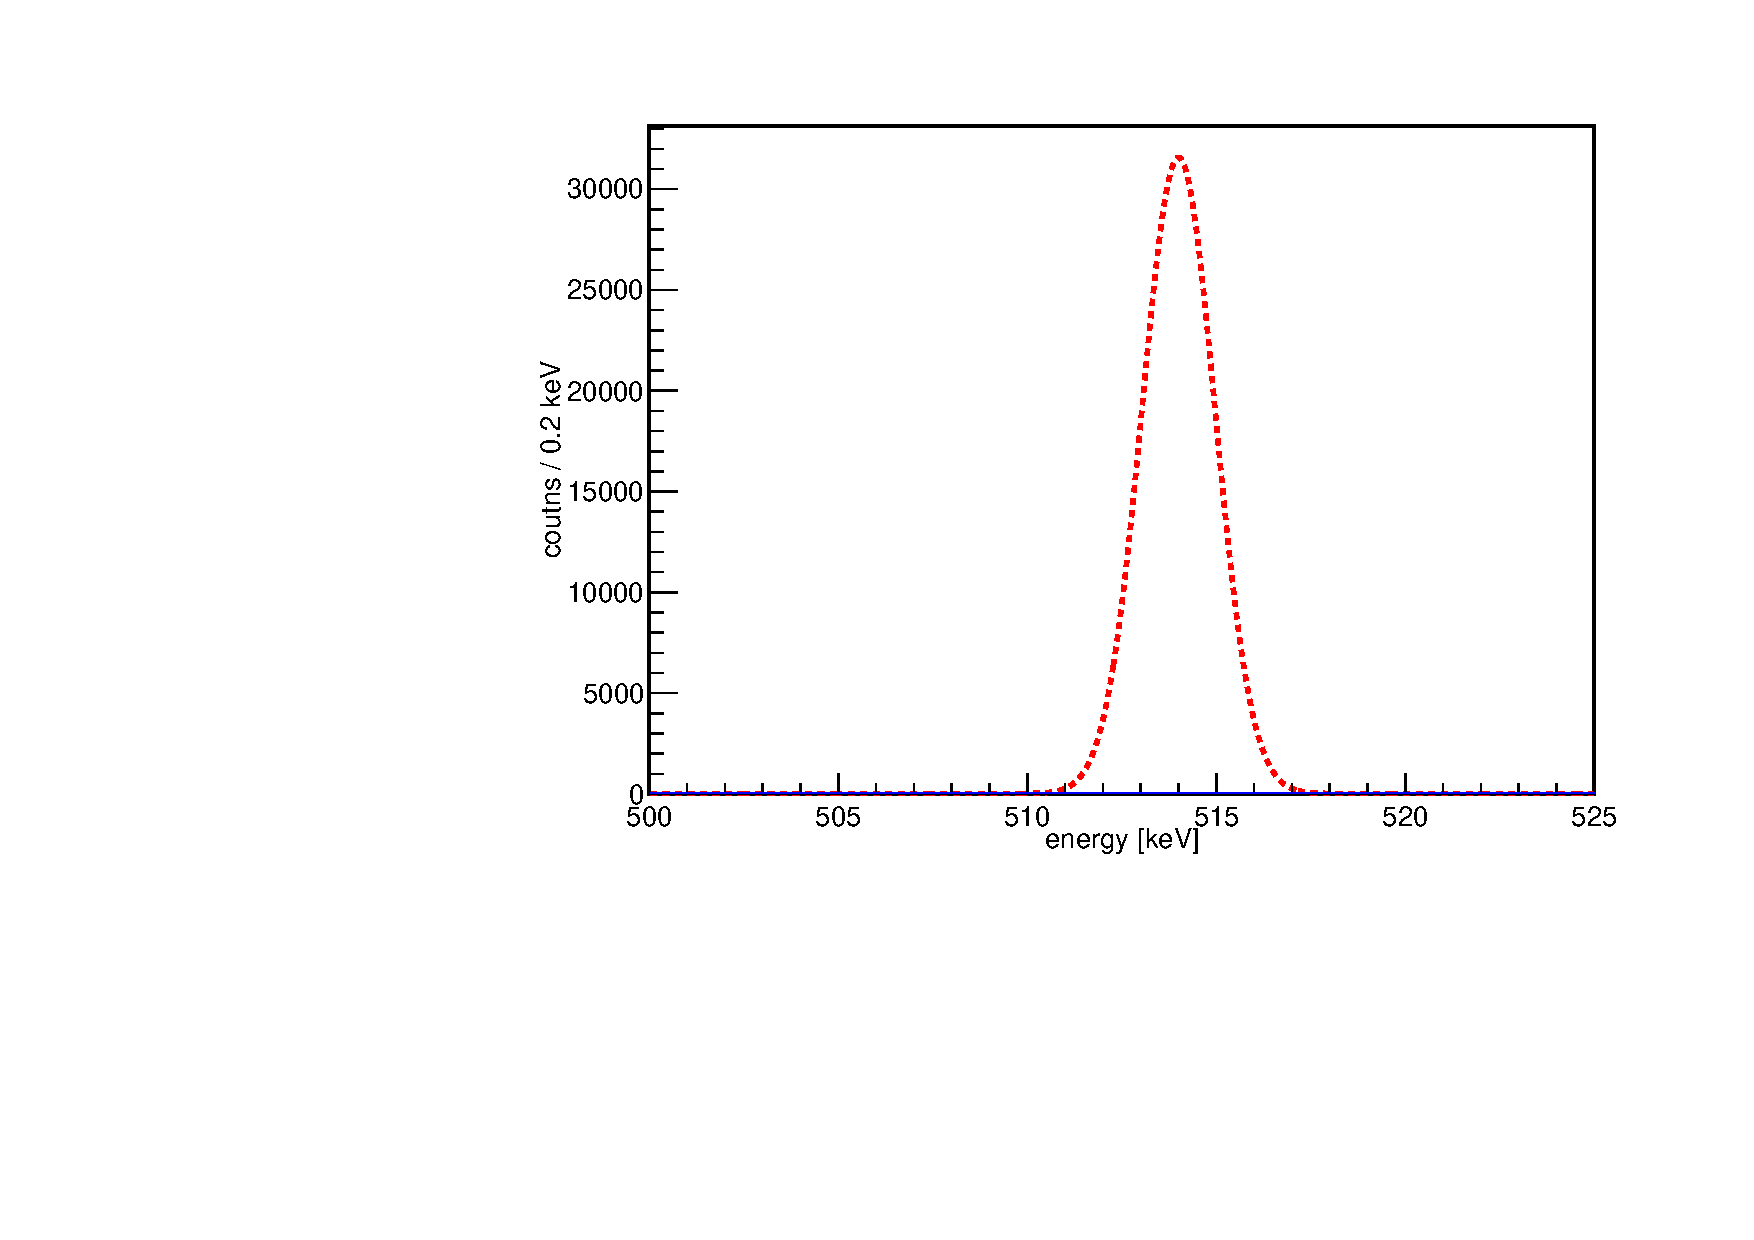
\includegraphics[width=75mm]{./Bilder/WARP.pdf}
		\caption{WARP}
		\label{fig:WARP}
	\end{subfigure}\hfill%
	\begin{subfigure}{.5\textwidth}
		\centering
		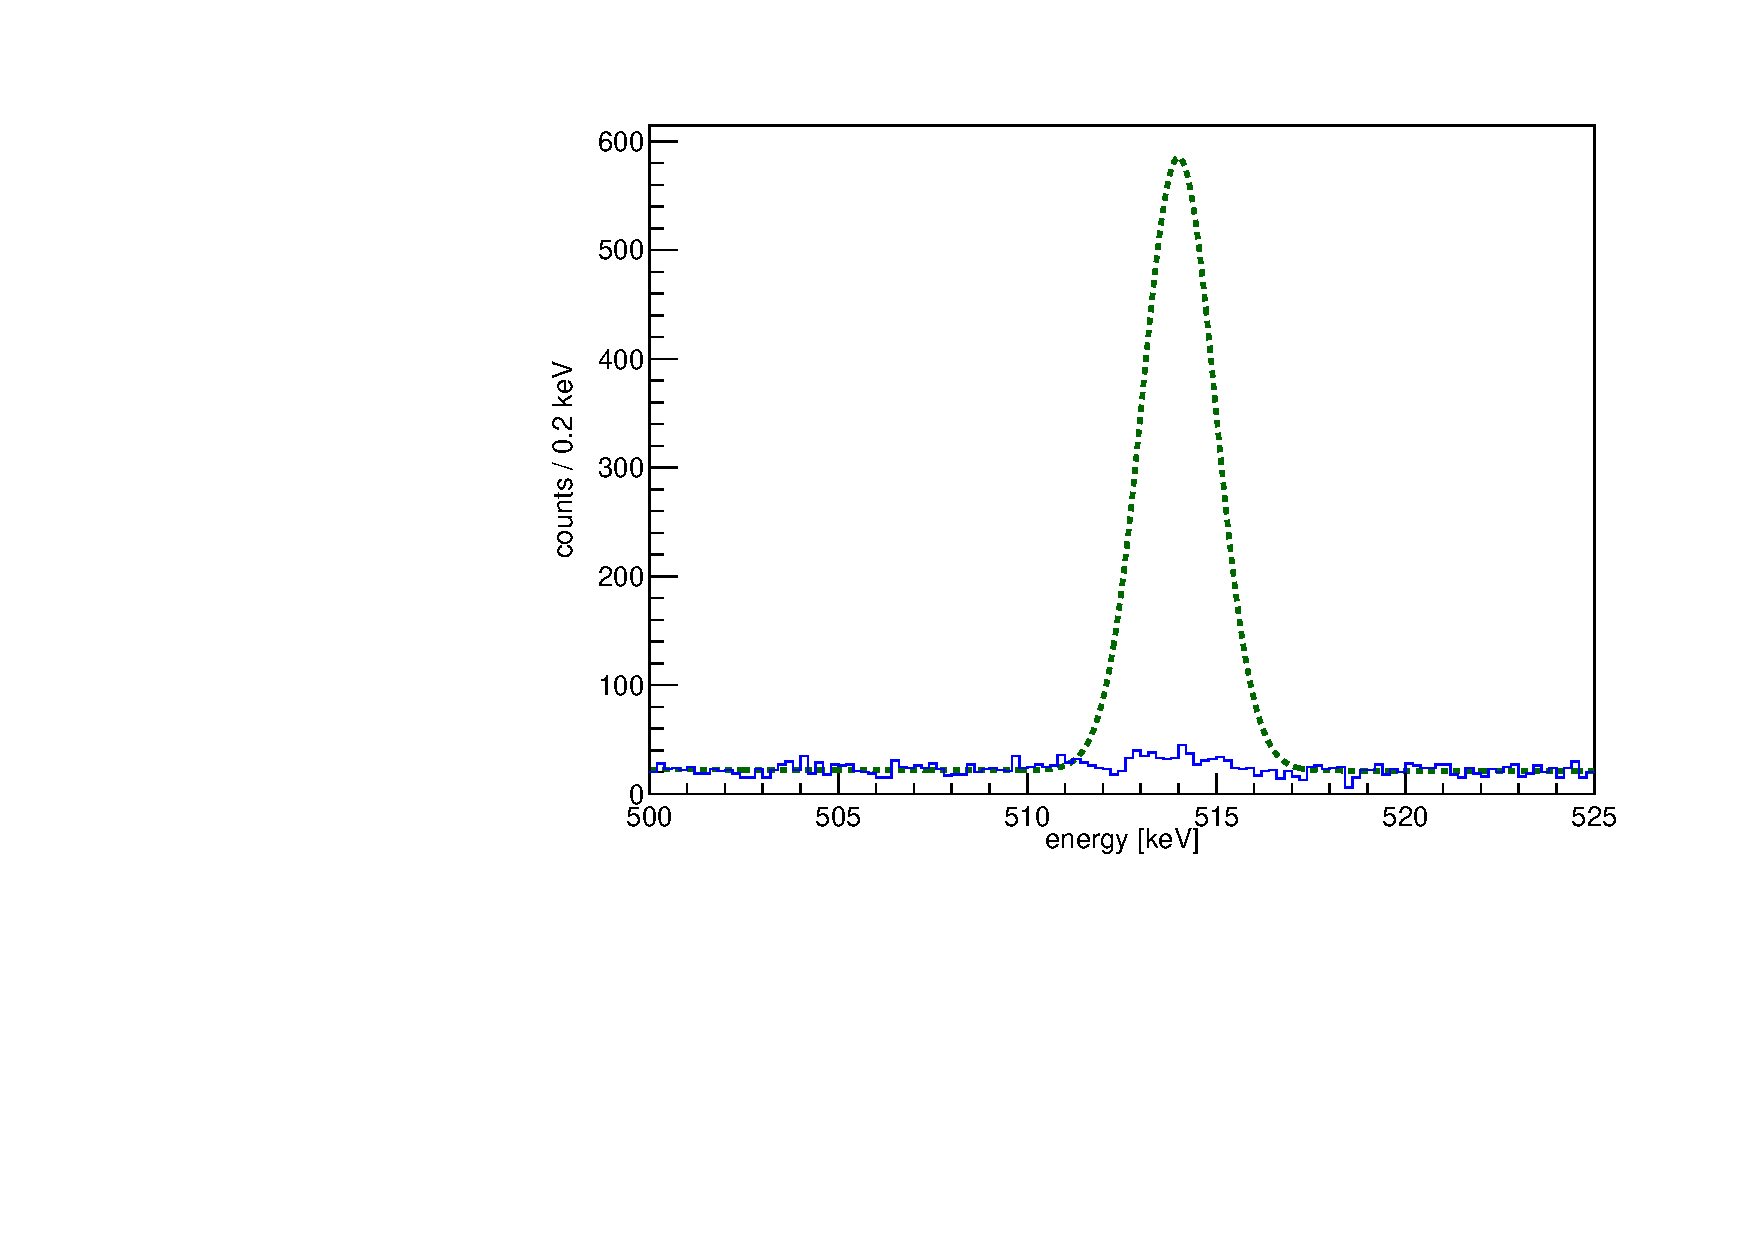
\includegraphics[width=75mm]{./Bilder/Darkside.pdf}
		\caption{Darkside}
		\label{fig:Darkside}
	\end{subfigure}
    \\
    \caption{
    	Energy spectra of the BEGe detectors from 500 to 525 keV.
    	The green plots in the spectra represent the theoretical peaks one could expect to measure if a specific activity of the respective experiment was present.
    	In both cases it would have created a much greater signal than observed above.
    	}
\end{figure}
\\

But why is the specific activity of \Kr\ in \gerda\ \PII\ so much smaller than in any other experiment?
As it was elaborated above, due to the argon being extracted from the atmosphere, \Kr\ should be present.
And the majority of the \Kr\ there should originate from nuclear power plants.
WARP's LAr also originated from the atmosphere but its specific activity was measured to be almost three orders of magnitude higher than \gerda's.
A possible explanation would be that the air from which the argon of WARP was extracted from was taken from a place with much a lot of nuclear power plants surrounding it while the argon of the \gerda\ experiment originated from air far away from any reactor.
On the other hand Darkside's argon originated from an underground reservoir where only natural fission decays produce any \Kr\.
But its specific activity is still much higher than \gerda's.
Also no extra purification of the LAr was applied.
This would mean that in the case of the LAr in \gerda\ one was extremely lucky to have found argon that had such low \Kr\ concentration that its impact on the background can basically be neglected.
\\

Now that a concrete value for the specific activity of \Kr\ has been determine the second attempt to measure the specific activity will described in the next chapter.
\\  
\fi



%	4.70E-04	8,87E-05	Bq/l


% calculate Amplitude of Gauss peak at 514keV and use factor from Monte Carlo Simulation to estimate

% look at phase diagram at range of 500 to 525 keV, use different filters and fit remaining data with Gaussian function
% -> get amplitude
% make a Monte Carlo simulation to estimate actual Kr85 activity in LAr from measured activity in detectors
% -> with amplitude and factors from MC-Simulation one can calculate the specific activity

























\chapter{Change in Count Rate over Time}
\label{sec:SAfromDecrease}

This chapter focuses on the second approach to determine the specific \Kr\ activity based on the change in the total count rate over time.
The previous chapter having already determined a value of $(0.508\pm0.086) \ \unit{mBq}/\unit{l}$ for \Kr's specific activity, the purpose of this second approach is to cross-check this value.
Because \Kr\ has a half-life of 10.739 yr, a decrease of $ 13\% $ in its count rate can be expected for a measurement period of 2.17 yr.
\nuc{Ar}{42} has a similar half-life as \Kr\ (32.9 yr) and, thus, presents the problem that its change should also be measurable \cite{chen_nuclear_2016}.
Its possible influence and that of other radioactive isotopes on the count rate is discussed in section \ref{sec:other}. 
But first, it is necessary to plot the count rate over time to estimate the order of magnitude for the total count rate and for every visible change, as described in section \ref{sec:plotting}.
Then, in section \ref{sec:monteCarlo2}, a Monte Carlo simulation is used to calculate whether any changes of this scale can occur considering the result of the previous chapter.
The last section will focus on fitting exponential decay functions of \Kr\ and \nuc{Ar}{42} through the diagram to determine which isotope may have caused a visible change.   
\\

\section{Plotting the Count Rate over Time}
\label{sec:plotting}

Whether or not \Kr's change is actually visible depends on whether the scale of the total count rate is in the same order of magnitude as \Kr's caused count rate or even lower.
If the total count rate measured would be in a higher order of magnitude than the change in count rate caused by \Kr, its change might not be distinguishable from statistical fluctuation.
A considerable portion of the total count rate can be reduced by selecting a suitable upper energy limit, as the influence of radioactive isotopes with a significantly higher Q value than \Kr's can be suppressed by doing so.
With the here selected upper limit of 400 keV, only a few \Kr\ events are lost, but the influence of many other radioactive isotopes can be suppressed, as this makes it easier to detect any change by \Kr. otherwise so that the detection of any change by \Kr.
\\

Additionally, some precautions had to be taken.
Together with the upper limit, it is also necessary to set a lower energy limit above the highest energy thresholds present in \PII.
This is done to suppress the influence of changes to the individual detector thresholds on the counting rate and was set to 200 keV.
As the count rate is also sensitive to the on/off settings of the detectors, it is necessary that only the data of detectors is used which have always been turned on.
For this reason, only the data sets of runs 55 to 92 have been used, as runs 53 and 54 only used a smaller number of detectors.
When considering the data of run 53 and 54, due to the lower number of detectors to use, the exposure is much lower at $21.9 \ \unit{kg}\cdot\unit{yr}$ compared to $41.5 \ \unit{kg}\cdot\unit{yr}$ when ignoring them.
The detectors used for this analysis are listed in table \ref{tab:Detector} in the appendix.
The standard \gerda\ analysis cuts have also been applied to the remaining data sets.
\\


\begin{figure}[t!]
	\centering
   	\begin{minipage}[t]{.475\textwidth}
		\centering
		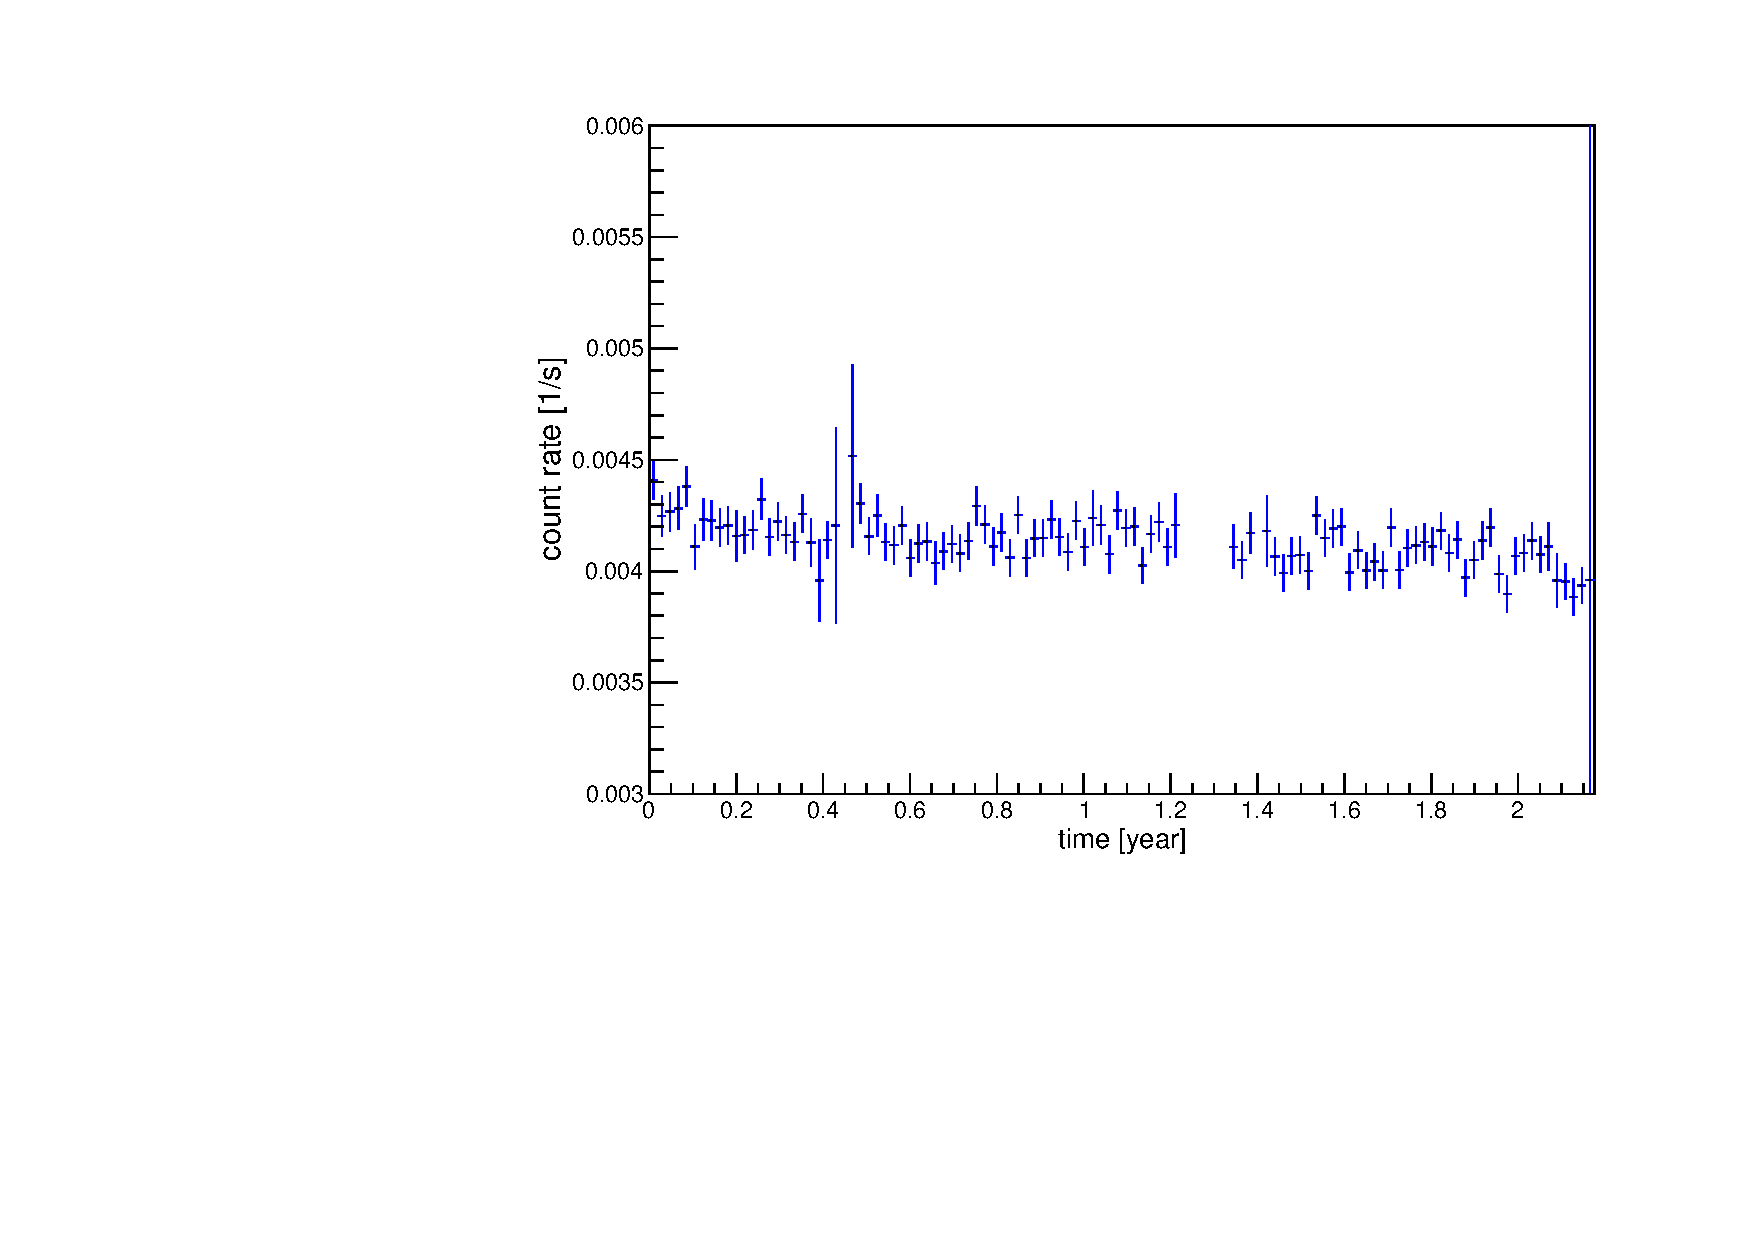
\includegraphics[width=\textwidth]{./Bilder/eventRate.pdf}
		\caption{Average count rate of each week plotted over the timeframe between run 55 and 92. }
		\label{fig:ChangeInEventRate}
	\end{minipage}\hfill%
	\begin{minipage}[t]{.475\textwidth}
		\centering
		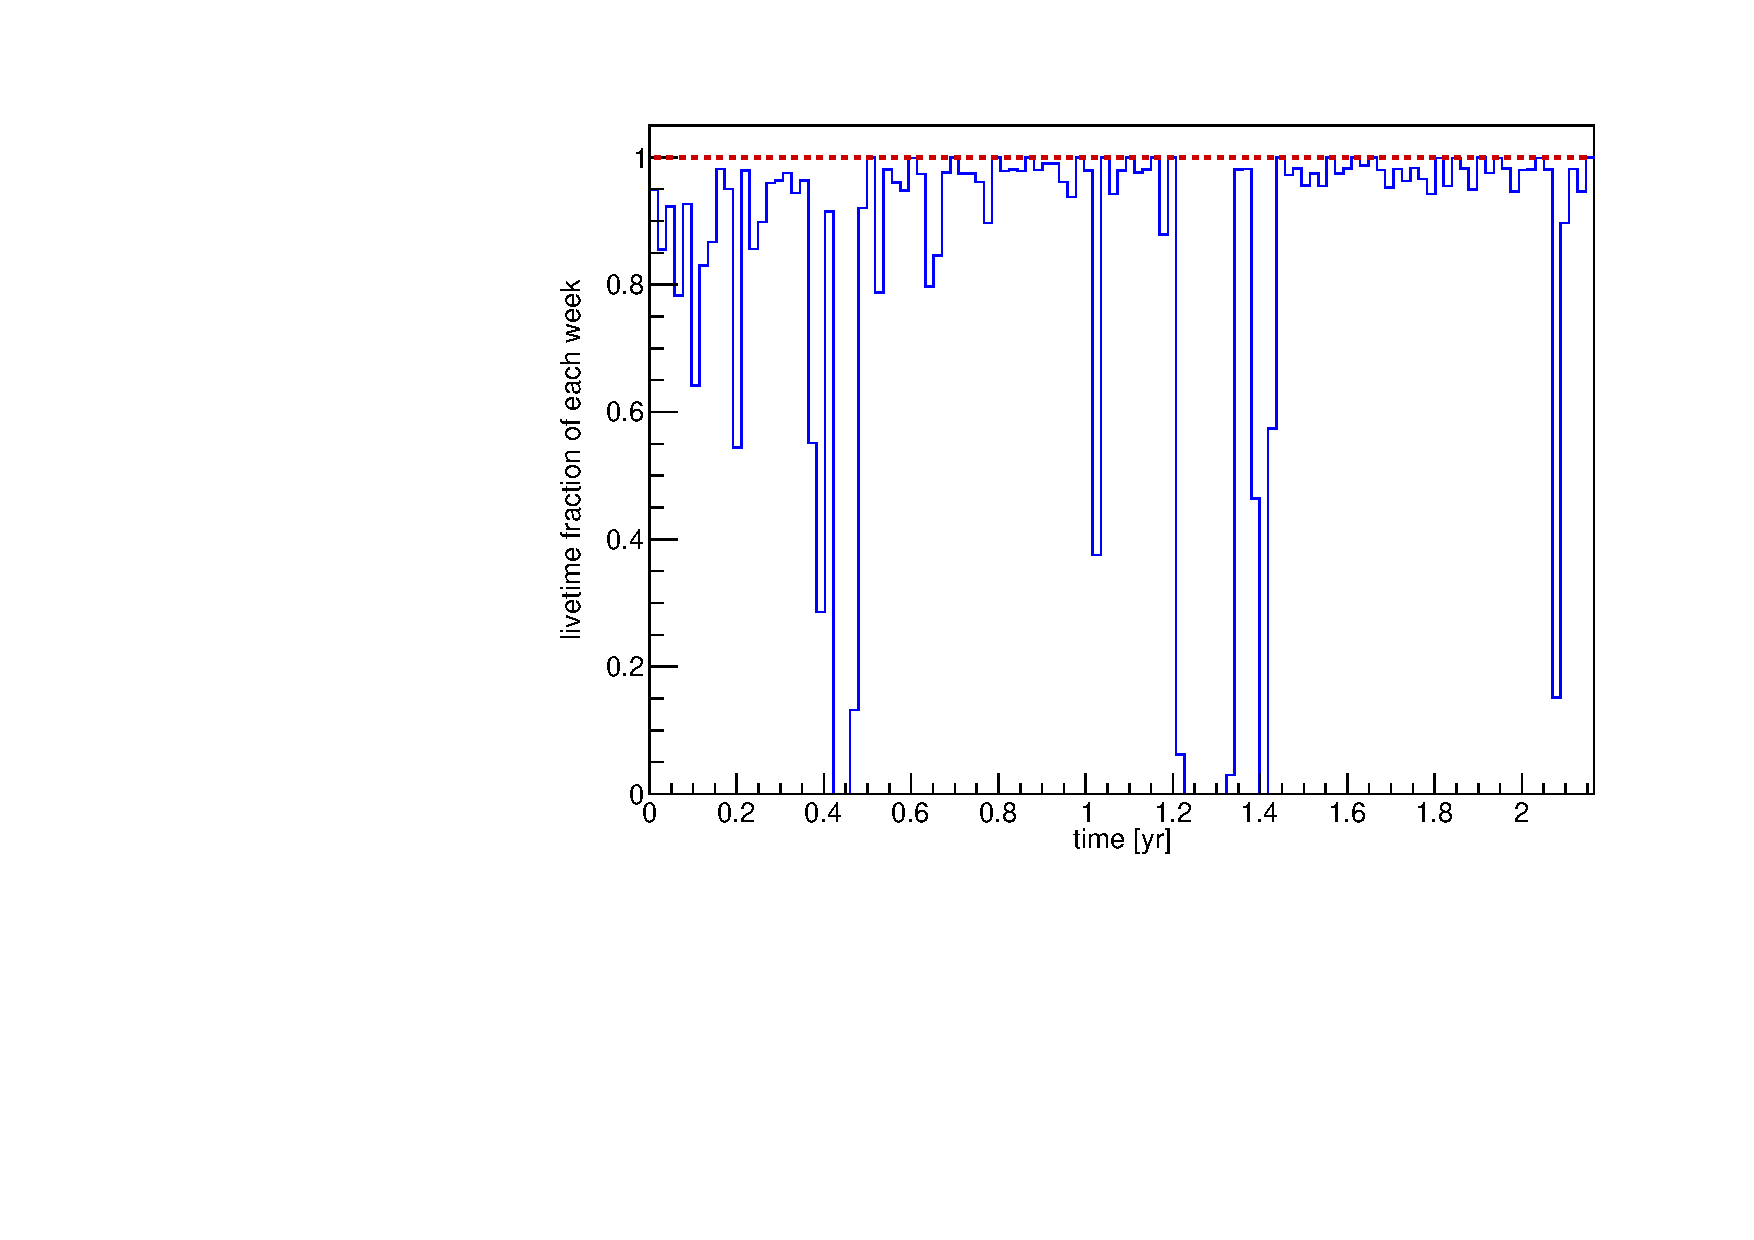
\includegraphics[width=\textwidth]{./Bilder/onceInALivetime.pdf}
		\caption{The lifetime fractions of the detectors in the respective week plotted over the timeframe between run 55 and 92.}
		\label{fig:lifetime}
	\end{minipage}
\vspace{5mm}
\end{figure}


It is now possible to create a diagram of the measured count rates as seen in figure \ref{fig:ChangeInEventRate}.
For this purpose, the number of counts measured in each week has to be determined and divided by the measurement time in the same week.
The measurement times have to be determined again by counting the number of test pulse signals in each week and by multiplying them by 20 seconds.
The lifetime fractions of each week can be seen in figure \ref{fig:lifetime}.
\\

The scale of the total count rate in diagram \ref{fig:ChangeInEventRate} is in the order of 10$^{-3} \unit{cts} / \unit{s}$.
A change in time of the same order of magnitude can be seen from its course.
\\

\section{Monte Carlo}
\label{sec:monteCarlo2}


Whether this order of magnitude in the change of the count rate is compatible with the results of the previous chapter must be determined with the aid of a Monte Carlo simulation.
With a conversion factor similar to the one derived from the previous simulation, the expected count rate for a given activity of \Kr\ can then be calculated.
The difference between the simulations, however, is that, this time, the actual \Kr\ decays are simulated instead of just the 514 keV gamma emissions.
\\

The detection efficiency determined by this simulation is also expected to be much smaller than earlier.
This is due to the much shorter range of the electrons in the LAr as well as their low transmission factor in germanium, leaving many electrons to be captured in the dead layer of the detectors.
For this reason, a much higher number of $N_{\mathrm{sim}}$ = 1 billion \Kr\ decays in a volume of $V_{sim} = 17.65 \ \mathrm{m}^3$ have been simulated.
\\

!!!!! soll der Paragraph raus?
Figure \ref{fig:Sim1Spektrum} shows the simulated energy spectrum of all measured events in the detectors considered.
One can see that the 514 keV gamma peak contains a relatively high number of counts for gammas only emitted in 0.434$\%$ of all \Kr\ decays.
This indicates that a disproportionate number of events in the range of 200 to 400 keV were caused by the 514 keV gamma.
Comparing the ratio of the values measured in this range divided by the line counts at 514 keV in the case of the two spectra \ref{fig:Sim1Spektrum} and \ref{fig:PhasenraumMC514}, it can be seen that only about 20.1$\%$ of all events in this energy interval were caused by beta radiation.
As the dead layer of the Monte Carlo simulation is only an approximation to the real dead layer, a systematic error is generated in the simulation.
However, since only a small number of events were caused by beta electrons, this error can be neglected, as the 514 keV gamma most likely deposits its energy deep in the active detector volume. 
\\

\begin{figure}[t!]
\centering
		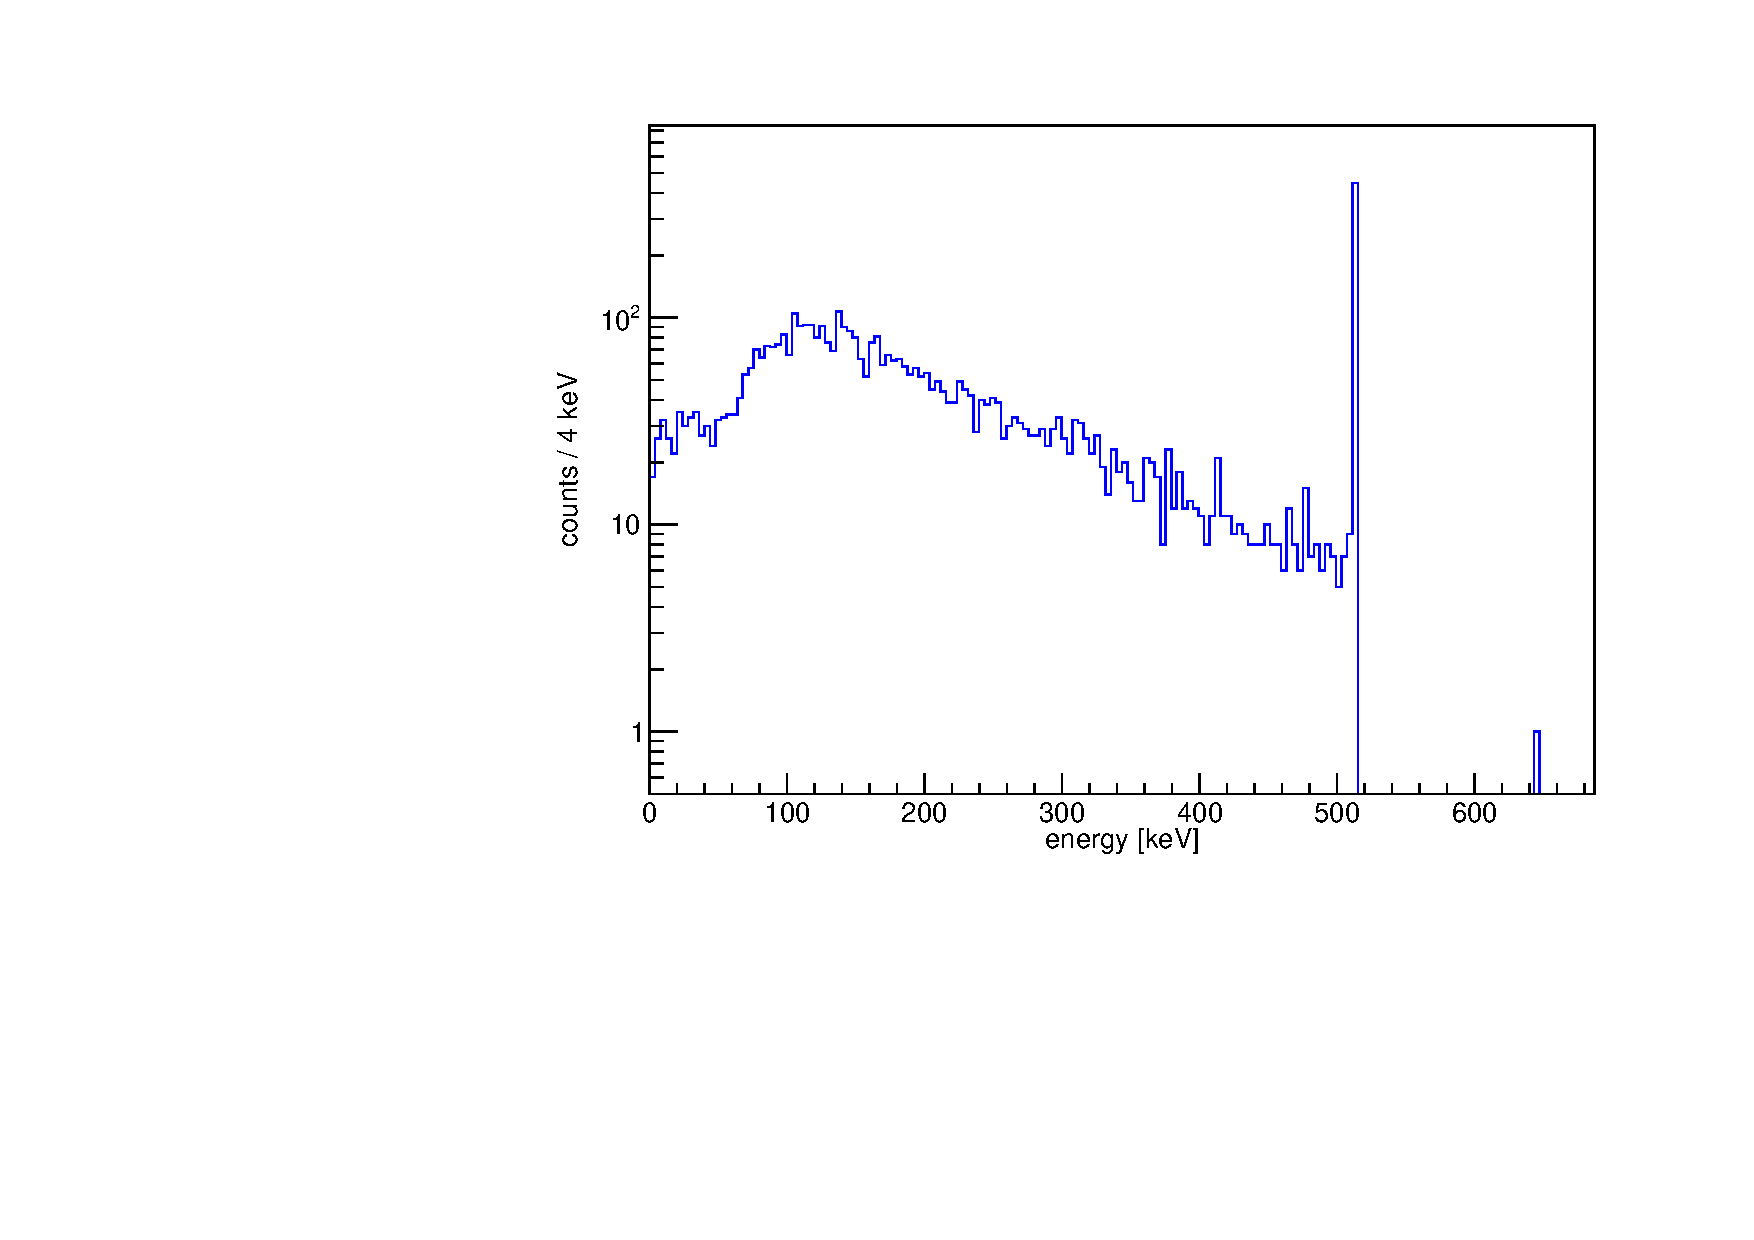
\includegraphics[width=0.6\textwidth]{./Bilder/Sim1Phasenraum.pdf}
		\caption{
			Measured energy spectrum of the 1 billion simulated \Kr\ decays. 
			The blue colored area represents the counts used for the calculation of the detector efficiency.
		}
		\label{fig:Sim1Spektrum}
		\vspace{5mm}
\end{figure}


The colored area of figure \ref{fig:Sim1Spektrum} contains a number of $\Delta N =$ 1438 counts.
This results in a detector efficiency of 
\begin{equation*}
\epsilon = \frac{\Delta N}{N_{\unit{sim}}} = (1.438 \pm 0.038) \times 10^{-6} \frac{\unit{cts}}{\unit{decay}}
\end{equation*}
Its reciprocal value and its division by the simulated volume result in the volume-independent conversion factor
\begin{equation*}
\frac{1}{\epsilon V_{\unit{sim}}} = (39.39 \pm 1.04) \frac{\unit{decay}}{\unit{cts \times l}}
\end{equation*}
In this case, it can still be assumed that this value is volume-independent, since the beta particles have an even shorter range than the gammas and since the same volume is used as in the previous simulation.
\\

The count rate expected for the previously determined specific activity can now be calculated as follows
\begin{equation*}
R_{^{85}\mathrm{Kr}} = \bar{a} \times  \epsilon V_{\mathrm{sim}} =  (1.29\pm0.25) \times 10^{-5} \frac{\unit{cts}}{\unit{s}}
\end{equation*}
\\

\section{Other Relevant Radioactive Isotopes}
\label{sec:other}

If one compares this value with the scale of the count rate diagram above, it can be seen that actually no change caused by \Kr\ should be visible over the statistical fluctuations of the measured count rate.
However, the fact that a change can be seen, leaves two possible scenarios.
Either the value determined in the first method was wrong and the specific \Kr\ activity in the LAr was actually much higher, or the assumption that \Kr\ was the only isotope with a significant change over time was wrong.
\\

There are three isotopes present at \gerda\ which are of interest here: \nuc{Po}{210}, \nuc{Ar}{39} and \nuc{Ar}{42}.
\nuc{Po}{210} has a much shorter half-life than \Kr\ with its $138 \ \unit{h}$, but this value is by far too small to expect a change in the examined interval \cite{kondev_nuclear_2008}. 
Furthermore, it has a Q-value far above 400 keV, so that this isotope can be neglected in general, as almost no decay should lead to an event in the expected energy range. 
\nuc{Ar}{39} is the most active isotope in this energy range, but has a much longer half-life of 269 yr, which means that no change should be visible in the studied time frame \cite{singh_nuclear_2014}.
\nuc{Ar}{42} has a half-life of 32.9 yr, but its specific activity has already been determined to be $0.148 \ \mathrm{mBq/l}$, which means, that at first glance, no change caused by it should be visible either \cite{chen_nuclear_2016}.
However, its also unstable daughter nucleus \nuc{K}{42} is positively charged right after its creation and is accelerated towards the detectors due to their electrostatic fields.
This results in a much higher \nuc{K}{42} density around the detectors and therefore a higher measurable specific activity.
As \nuc{K}{42} has a much lower half-life than \nuc{Ar}{42}, any change in \nuc{Ar}{42}'s activity also immediately changes \nuc{K}{42}'s activity.
This means \nuc{Ar}{42}'s change over time gets effectively amplified in the count rate diagram to a level that it could possibly cause the change seen.
\\

\section{Fitting}
\begin{figure}[t!]
	\centering
	\begin{subfigure}[t]{.475\textwidth}
		\centering
		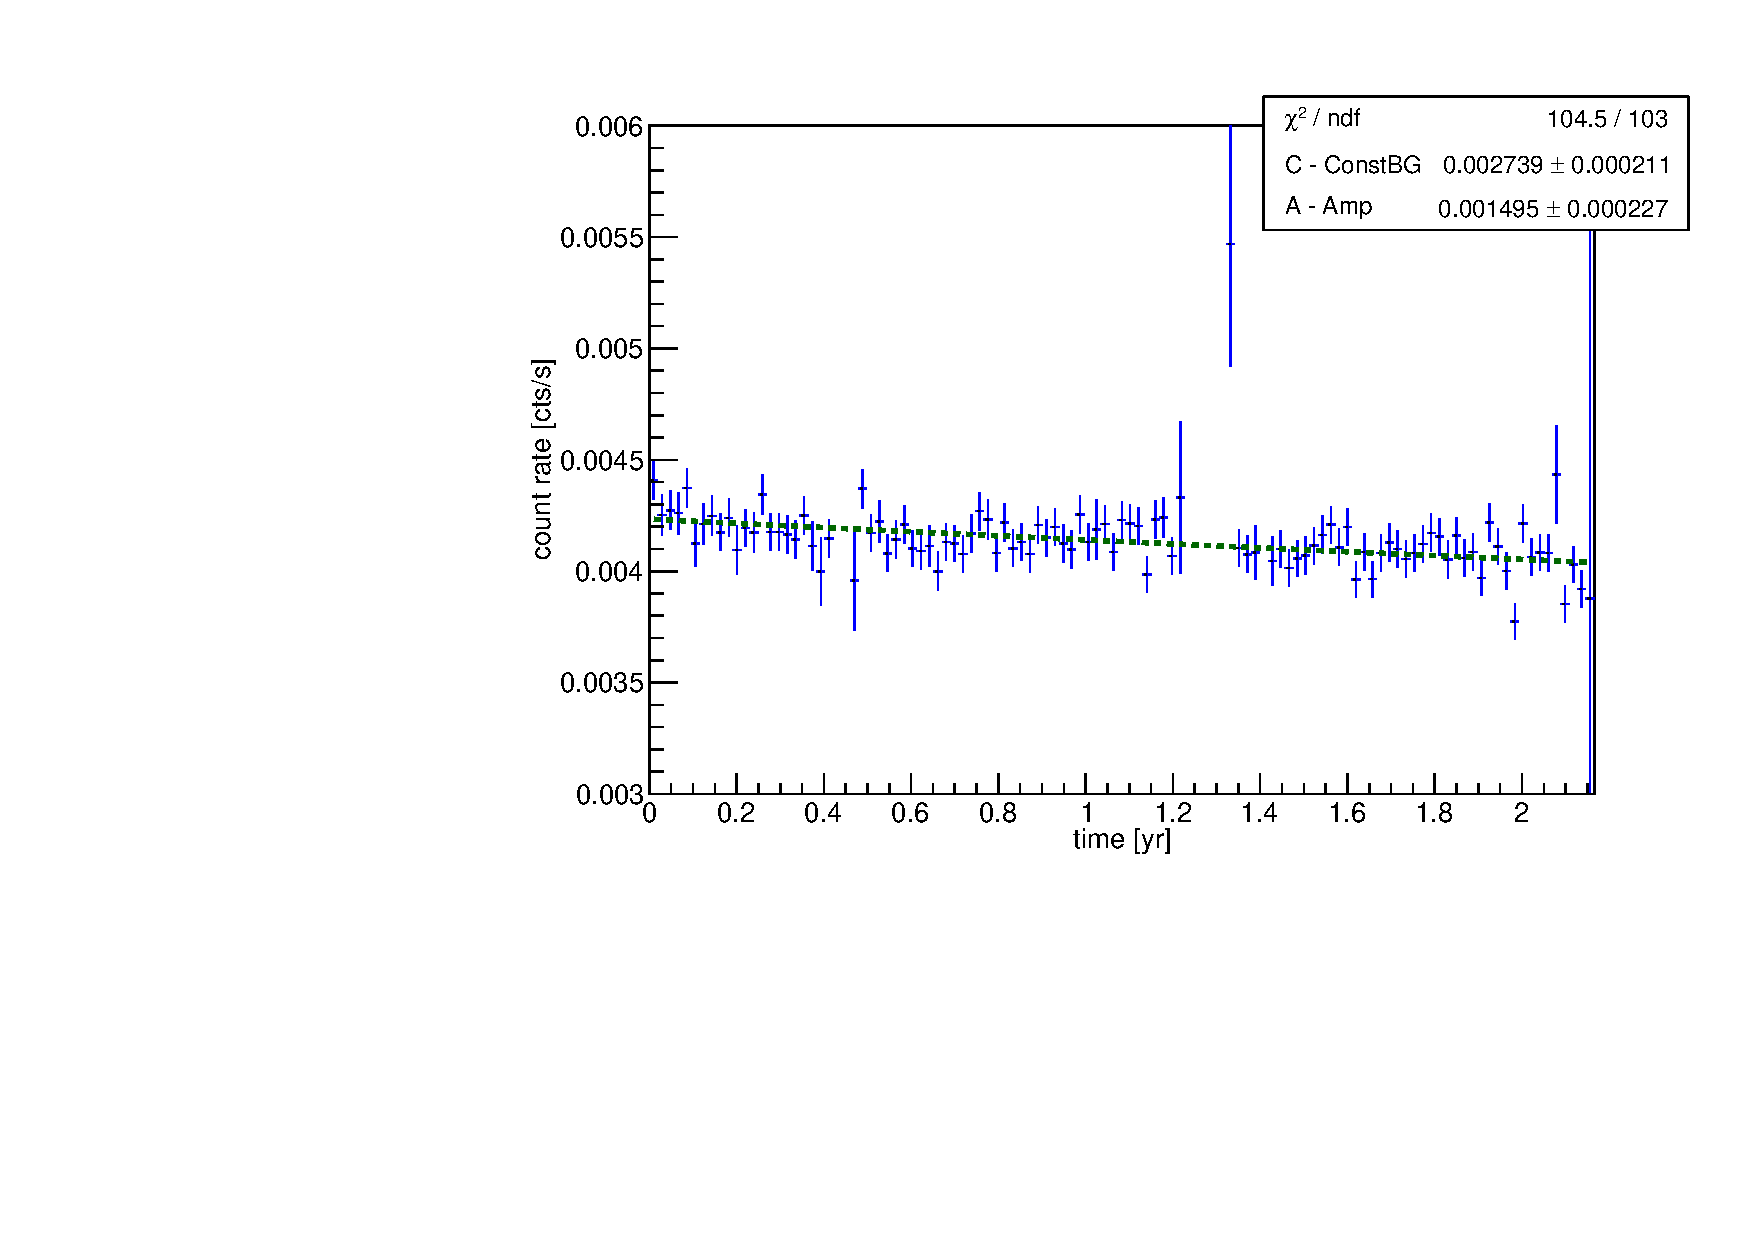
\includegraphics[width=\textwidth]{./Bilder/eventRateFit.pdf}
		\caption{ \Kr\ }
		\label{fig:eventRateFit}
	\end{subfigure}\hfill%
	\begin{subfigure}[t]{.475\textwidth}
		\centering
		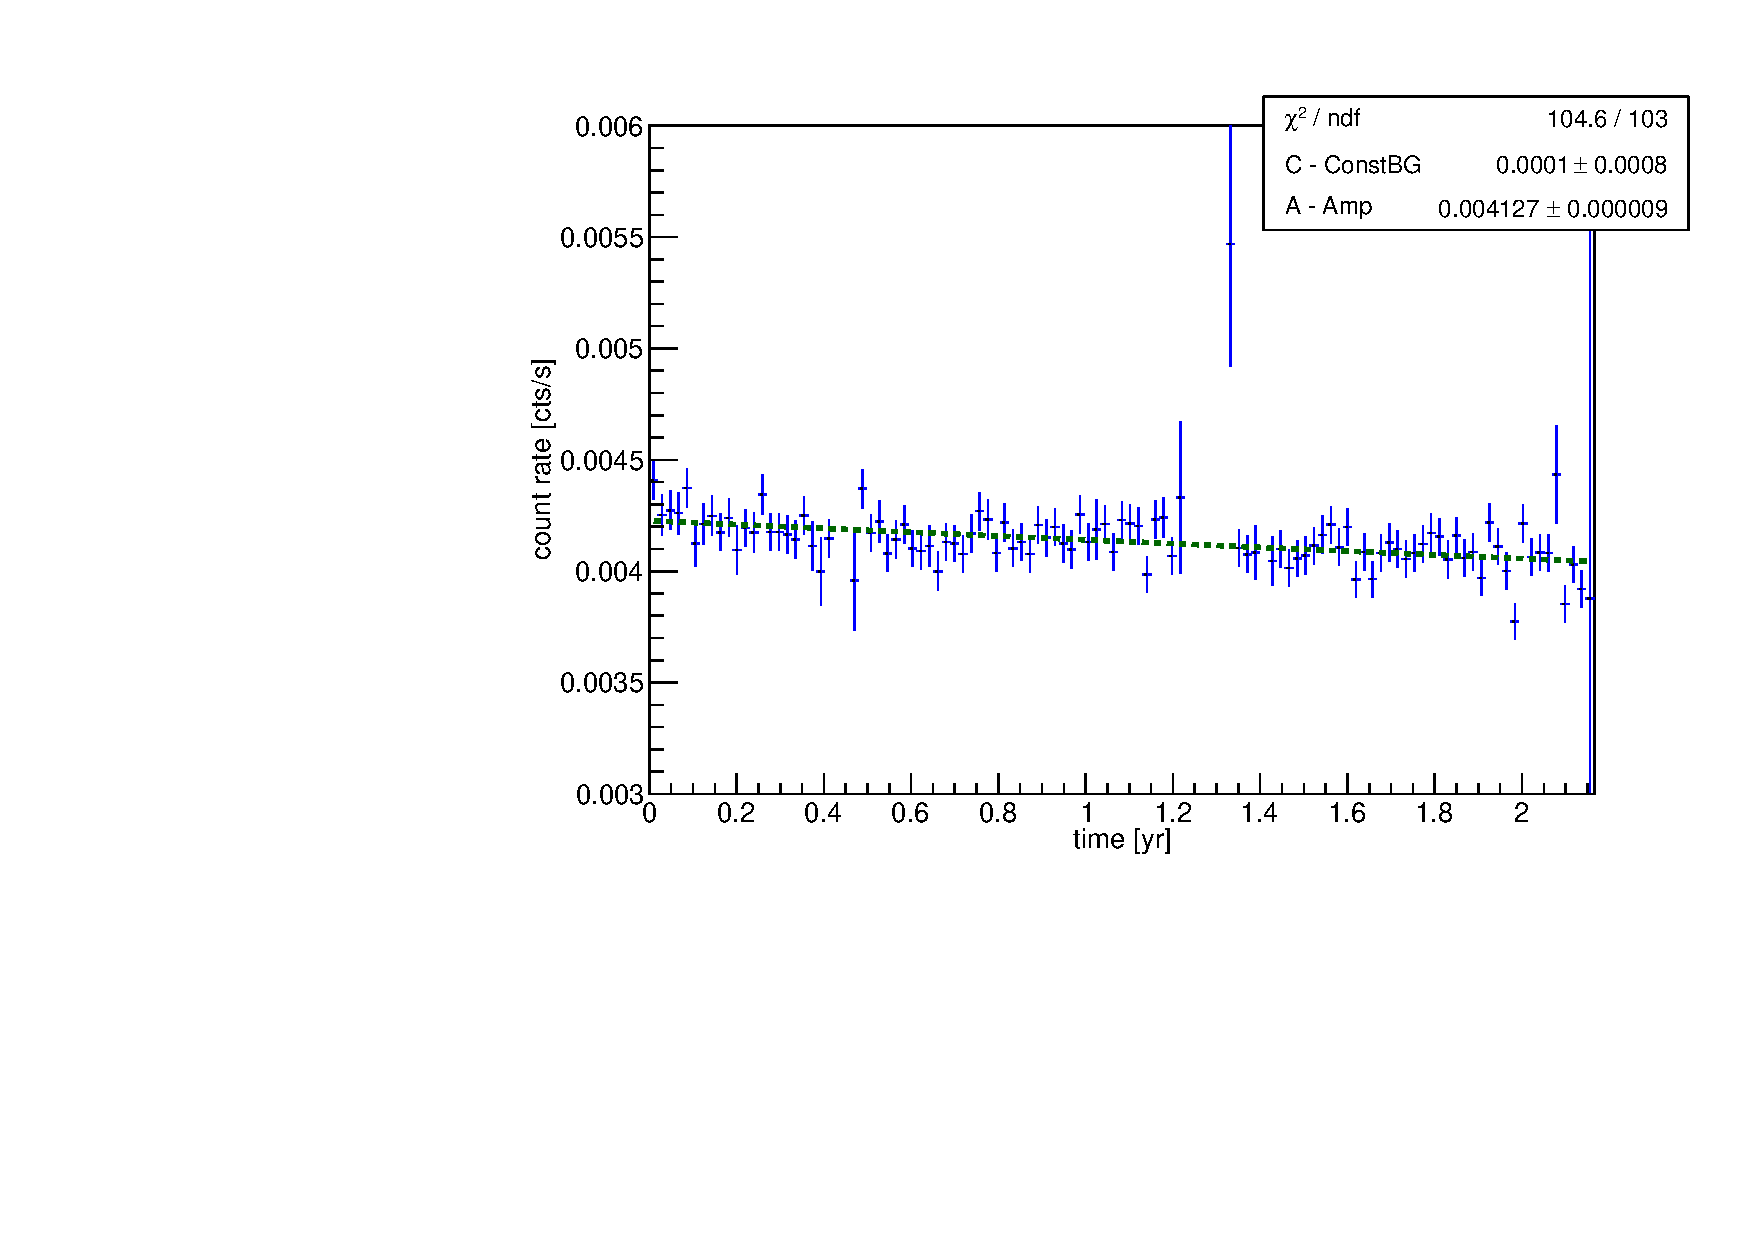
\includegraphics[width=\textwidth]{./Bilder/Argon.pdf}
		\caption{
		$^{42}$Ar
		}
		\label{fig:Argon}
	\end{subfigure}
	\caption{Fitted count rate graph using function \ref{equ:FitFun} with parameter B fixed on the half-lives of the respective radioactive isotope.}
		\label{fig:fit2}
		\vspace{5mm}
\end{figure}
To find out whether the change was caused by \Kr\ or \nuc{Ar}{42}, it is necessary to fit  plot \ref{fig:lifetime} with the respective exponential decay functions of the two isotopes.
From the goodness of the two fits it should be possible to determine which isotope describes the measured data better.
Function \ref{equ:FitFun} was used for the fits with parameter B fixed to the respective half-lives of the two isotopes.
\begin{equation}
\mathrm{f}(x) = \mathrm{A}\times\exp\left(-\frac{\log(2)}{\mathrm{B}} x \right) + \mathrm{C}
\label{equ:FitFun}
\end{equation}
The resulting fitting plots can be seen in figures \ref{fig:eventRateFit} and \ref{fig:Argon}.
From the resulting amplitude in the \Kr\ fit, a specific activity of $(58.9\pm10.5) \  \unit{mBq}/\unit{l}$ can be calculated using the conversion factor.
This value is, as expected, much higher than determined in the previous chapter.
Since no Monte Carlo simulation can be calculated for \nuc{K}{42} as it is not homogeneously distributed in LAr, no statement can be made about its specific activity.
\\

Concerning the goodness of the fit, the chi-squared $\chi^2$ value of the two fit functions can be evaluated.
The smaller this value, the better the fit function describes  the measured data.
However, in this case, both fit functions seem to have a similar $\chi^2$ value and therefore describe the course of the data equality well.
This leads to the conclusion that the data used in this method does not have enough statistical value to be able to discriminate which of the two isotopes is responsible for the change.
Therefore, no statement can be made about the specific activity of \Kr\ from this change in count rate.
With more measuring time it might be possible to make a statement about the responsible isotope and to potentially falsify the result of found above.
\\

Since \nuc{K}{42} has a much higher Q value ($Q_{\beta} = 3525.22 \ \unit{keV}$ \cite{chen_nuclear_2016}) than \Kr, it should be possible to choose another energy frame above \Kr's Q-value and to determine its change in the count rate there without \Kr's influence.
However, since no Monte Carlo simulation can be calculated for \nuc{K}{42}, no statement can be made about the expected count rate in the previous energy frame.








% use fit to calculate the decrease in rate of the signals in range from 200 to 500keV
% from fit and assumption that only Kr85's activity is decreasing one can calculate the specific activity from the amplitude of the fit

% use Volume of LAr-Tank to determine the number of Kr85 and from this the concentration in the argon

\chapter{Conclusion, Comparison and Outlook}
\label{sec:ConcAndOutlook}
\section{Conclusion}

With the line count rate analysis, it was possible to show that the specific activity of \nuc{Kr}{85} in the LAr in \gerda\ \PII\ has a value of $(0.508\pm0.086) \ \unit{mBq} / \unit{l}$.
The attempt to verify this number using the half life did not work.
Due to \Kr's low value, only a strong discrepancy could have been detected.
However, the presence of \nuc{Ar}{42} with a similar decay time and its daughter nuclei \nuc{K}{42} did not allow to confirm or falsify the value of the previous method.

\\
\section{Comparison to WARP and Darkside}

Two other experiments, also using LAr, were mentioned at the end of the introduction chapter: the Darkside experiment using UAr and the WARP experiment also using argon from the atmosphere.
It was assumed earlier that Darkside's specific \Kr\ activity was two orders of magnitude smaller than in the WARP experiment as the UAr did not come into contact with the man-made \Kr.
Surprisingly, however, \gerda\ measured a much lower specific \Kr\ activity than WARP or Darkside while also using argon originating from the atmosphere.
\\

Besides the activities themselves, one could also chose an alternative way and calculate how high the line count rates would have been in the \gerda\ setup if the specific activities of WARP and Darkside were present.
In section \ref{sec:Fitting} a line count of about 180 counts was found at 514 keV.
The corresponding line count from the specific activities of the other experiments can then be determined by upscaling the line count measured in \gerda\ to the corresponding values with the factor ($\bar{a}_{\mathrm{Exp}}/\bar{a}_{\mathrm{GERDA}}$).
This results in a line count of about $\mathcal{O}(1000)$ in the Darkside experiment and about $\mathcal{O}(50000)$ in the WARP experiment, which means, that a much higher peak could have been measured.
\\

Moreover, one can now also determine the expected count rate from the second method.
Since the specific \Kr\ activity of Darkside is only one order of magnitude higher than that of \gerda, one should hardly see any change here either.
On the other hand, one can calculate an expected count rate for WARP in the order of 10$^{-3} \  \unit{cts} / \unit{s}$, so in this case a significant change should be recognizable.
\\

To gain further insight into why the specific \Kr\ activity in \gerda\ can be so much lower, one could study the purification process during filling of the \gerda\ cryostat before starting with \PI.
The concentration of \Kr\ already being much smaller before the gas separation is very unlikely due to  \Kr\ being relatively homogeneously distributed in the atmosphere \cite{j._jacob_atmospheric_1987}.
\\



\section{Outlook}
Also mentioned in the introduction, the \gerda\ experiment is planned to keep measuring until 2020.
Afterwards the \gerda\ setup will be converted into the LEGEND experiment that will further investigate the \onbb\ decay in \nuc{Ge}{76} and will use a new LAr filling.
It is therefore possible that in LEGEND a much higher concentration of \Kr\ may be present again and, thus, the radioactive background in the lower energy range may be larger.
This would result in a much higher contribution of \Kr\ to the background of a low energy analysis.
\\





%%%%%%%%%%%%%%%%%%%%%%%%%%%%%%%%%%%%%%%%%%%%%%%%%%%%%%%%%%%%%%%%%%%%%%%%%%%%%%%%
% -----------------------------------------------  ADD SOME ACKNOWLEDGMENTS  ---
%%%%%%%%%%%%%%%%%%%%%%%%%%%%%%%%%%%%%%%%%%%%%%%%%%%%%%%%%%%%%%%%%%%%%%%%%%%%%%%%
\newpage
\section*{Acknowledgments}

%%%%%%%%%%%%%%%%%%%%%%%%%%%%%%%%%%%%%%%%%%%%%%%%%%%%%%%%%%%%%%%%%%%%%%%%%%%%%%%%
%%%%%%%%%%%%%%%%%%%%%%%%%%%%%%%%%%%%%%%%%%%%%%%%%%%%%%%%%%%%%%%%%%%%%%%%%%%%%%%%

%----------------------------------------------------------------- appendix ----
%%%%%%%%%%%%%%%%%%%%%%%%%%%%%%%%%%%%%%%%%%%%%%%%%%%%%%%%%%%%%%%%%%%%%%%%%%%%%%%%
% --------------------------------------------------- ADD APPENDIX (IN CASE) ---
%%%%%%%%%%%%%%%%%%%%%%%%%%%%%%%%%%%%%%%%%%%%%%%%%%%%%%%%%%%%%%%%%%%%%%%%%%%%%%%%
\appendix

\section{Determining the resolution of the detector types}
\label{sec:ResDetermination}
rgdagadgadgdsgdsgrsgserg



% \section{}
% \label{}

%--------------------------------------------------------------- references ----
\backmatter
\printbibliography
%\bibliographystyle{unsrt}
%\bibliography{references}
\listoffigures

\end{document}
